\documentclass[12pt]{book} 

\usepackage{cite}
\usepackage{graphicx}
\usepackage{geometry}
\usepackage{indentfirst} % indent first line
\usepackage{amsmath,amsthm,amsfonts,amssymb} % ams
\usepackage[normalem]{ulem} % underline emphasize
\usepackage{bm} % bold math
\usepackage{multirow} % multi row in table
\usepackage{color} % colored link
\usepackage{makeidx} % index
\usepackage[linewidth=1pt,nobreak=true]{mdframed} % box around a content
\usepackage[titletoc]{appendix} % appendix
\usepackage{enumitem} % enumerate
\usepackage{simplewick} % wick diagram
\usepackage{tikz-cd}  % commutive diagram
\usepackage{diagbox} % slash in table
\usepackage[colorlinks]{hyperref} % color the hyperref
\usepackage{xeCJK} % Chinese support

\allowdisplaybreaks[4]  % allow to break equations 
\geometry{left=1.5cm,right=2.0cm,top=2.8cm,bottom=2.8cm}



\renewcommand{\ULdepth}{3pt}  %set uline depth
\newtheorem{theorem}{Theorem}[section]  %set theorem counter
\newtheorem{lemma}[theorem]{Lemma}  %set lemma counter
\newtheorem{axiom}[theorem]{Axiom}  %set axiom counter
\newtheorem{example}[theorem]{Example}  %set example counter
\newtheorem{method}[theorem]{Method}  %set method counter
\newtheorem{definition}[theorem]{Definition}  %set definition counter
\newtheorem{corollary}[theorem]{Corollary}  %set corollary counter
\renewcommand\arraystretch{1.2}  % set table height

\newenvironment{myTabuler}{  %tabular with space
	\vspace{2ex}
	\begin{tabular}
		}{
	\end{tabular}
	\vspace{2ex}
}


\title{Topology} 
\author{Wang Chao}
\makeindex
\begin{document} 

\maketitle 
\tableofcontents

\part{Set Thoery}
\chapter{Axioms of Zermelo-Fraenkel}
The axioms of Zermelo-Fraenkel (ZF) admits one kind of objects, namely {\bf sets}. Some times we also call a set of sets a {\bf family} of sets. We introduce the informal notion of {\bf class}, describe the objects that satify a fomula. A class that is not a set is called a {\bf proper class}.

The axioms of ZF together with the axiom of choice include:
\begin{axiom}[ZFC]
	\
	\begin{enumerate}
		\item {\bf Axiom of Extensionality}: If $X$ and $Y$ have the same elements, then $X=Y$.
		\item {\bf Axiom of Pairing}: For any $a$ and $b$ there exists a set $\{a,b†\}$ that contains exactly $a$ and $b$.
		\item {\bf Axiom Schema of Separation}: If $\phi(u,p)$ is a property with parameter $p$, then for any $X$ and $p$, there exists a set $Y=\{u\in X|\phi(u,p)\}$ that contains all those $u\in X$ that have the property $\phi$.
		\item {\bf Axiom of Union}: For any $X$ there exists a set $Y=\bigcup X$, the union of all elements of $X$.
		\item {\bf Axiom of Power Set}: For any $X$ there is exists a set $Y=P(X)$, the set of all subsets of $X$.
		\item {\bf Axiom of Infinity}: There exists an infinite set.
		\item {\bf Axiom of Schema of Replacement}: If a class $F$ is a function, then for any $X$ there exists a set $Y=F(X)=\{F(x)|x\in X\}$.
		\item {\bf Axiom of Regularity}: Every nonempty $X$ has an element disjoint from $X$.
		\item {\bf Axiom of Choice}: Every family of nonempty sets has a choice function.
	\end{enumerate}
\end{axiom}

The Axioms 1-7 are explained in detail as follows.
\section{Axiom of Extensionality}
\begin{axiom}
	If $X$ and $Y$ have the same elements, then $X=Y$:
	\begin{equation}
		\forall u(u\in X\leftrightarrow u\in Y)\rightarrow X=Y
	\end{equation}
\end{axiom}
\section{Axiom of Pairing}
\begin{axiom}
	For any $a$ and $b$ there exists a set $c$ that contains exactly $a$ and $b$:
	\begin{equation}
		\forall a\forall b\exists c\forall x(x\in c\leftrightarrow x=a\vee x=b)
	\end{equation}
	By extensionality, the set $c$ is unique.
\end{axiom}
\begin{definition}
	We can define the {\bf pair} 
	\begin{equation}
		\{a,b\}={\rm the\ unique\ }c{\rm\ such\ that\ } \forall x(x\in c\leftrightarrow x=a\vee x=b)
	\end{equation}
	The singleton $\{a\}$ is the set $\{a,a\}$.
\end{definition}
\begin{definition}[Kuratowski]
	We can define the {\bf ordered pair} 
	\begin{equation}
		(a,b)=\{\{a\},\{a,b\}\}
	\end{equation}
	
	We can further define n-tuples $(a_1,\dots, a_n)=(\dots((a_1,a_2),a_3)\dots,a_n)$
\end{definition}
\begin{theorem}
	Let $(a_1,\dots, a_n)$ and $(b_1,\dots, b_n)$ be two n-tuples.
	\begin{equation}
		(a_1,\dots, a_n)=(b_1,\dots, b_n)\leftrightarrow (a_1=b_1\wedge\dots\wedge a_n=b_n)
	\end{equation}
\end{theorem}
\begin{proof}
	If $(a,b)=(c,d)$, then $\{a\}=\{c\}$ or $\{a\}=\{c,d\}$. If $\{a\}=\{c,d\}$, then $a=c=d$ and $\{a,b\}=\{c\}=\{c,d\}$. So $a=b=c=d$. If $\{a\}=\{c\}$, then $\{a,b\}=\{c,b\}=\{c,d\}$. So $b=d$. In conclusion $(a,b)=(c,d)\rightarrow a=b\wedge c=d$. When $n>2$, use induction.
\end{proof}

\section{Axiom Schema of Separation}
\begin{axiom}
	Let $\phi(u,p)$ be a formula. For any $X$ and $p$, there exists a set $Y=\{u\in X|\phi(u,p)\}$:
	\begin{equation}
		\forall X\forall p\exists Y\forall u(u\in Y\leftrightarrow u\in X\wedge \phi(u,p) )
	\end{equation}
\end{axiom}
\begin{definition}
	We define the {\bf intersection} of $X$ and $Y$ as
	\begin{equation}
		X\cap Y=\{u\in X|u\in Y\}
	\end{equation}
	
	Clearly $X\cap Y=Y\cap X$
\end{definition}
\begin{definition}
	Let $C$ be a nonempty class of sets, we have the set called the intersection of $C$
	\begin{equation}
		\bigcap C=\{u\in X_0|u\in X {\rm\ for\ every\ } X\in C\}
	\end{equation}
	where $X_0\in C$. Clearly $\bigcap C$ is independent on the choice of $X_0$.
\end{definition}
\begin{definition}
	We define the {\bf difference} of $X$ and $Y$ as
	\begin{equation}
		X- Y=\{u\in X|u\not\in Y\}
	\end{equation}
\end{definition}
\section{Axiom of Union}
\begin{axiom}
	For any $X$ there exists a set $Y=\bigcup X$, the union of elements of $X$:
	\begin{equation}
		\forall X \exists Y\forall u (u\in Y\leftrightarrow (\exists z\in X) u\in z)
	\end{equation}
\end{axiom}
Now we can define 
\begin{equation}
	X\cup Y=\bigcup\{X,Y\},\ X\cup Y\cup Z=(X\cup Y)\cup Z,\ \dots
\end{equation}
and
\begin{equation}
	\{a_1,\dots,a_n\}=\{a_1\}\cup\dots\cup\{a_n\}
\end{equation}
\begin{definition}
	We define the {\bf symmetric difference} of $X$ and $Y$ as
	\begin{equation}
		X\triangle Y=(X-Y)\cup(Y-X)
	\end{equation}
\end{definition}
\section{Axiom of Power Set}
\begin{definition}
	A set $U$ is a {\bf subset} of $X$, written as $U\subseteq X$, if
	\begin{equation}
		\forall z(z\in U\rightarrow z\in X)
	\end{equation}
	
	If $U\subseteq X$ and $U\neq X$, then $U$ is a {\bf proper subset} of $X$.
\end{definition}

\begin{axiom}
	For any $X$ there is exists a set $Y$:
	\begin{equation}
		\forall X\exists Y\forall u (u\in Y\leftrightarrow u\subseteq X).
	\end{equation}
	
	Clearly such set is unique for any $X$. It's called the {\bf power set} of $X$, denoted by $P(X)$.
\end{axiom}
\begin{definition}
	The {\bf Cartesian product} of $X$ and $Y$ is the set
	\begin{equation}
		X\times Y=\{(x,y)\in PP(X\cup Y)|x\in X\wedge y\in Y\}
	\end{equation}
	
	Similarly let
	\begin{equation}
		X_1\times X_2\times\dots\times X_n=\{(x_1,\dots,x_n)\in \underbrace{P\dots P}_{n}(X_1\cup\dots\cup X_n)|x_1\in X_1\wedge\dots\wedge x_n\in X_n\}
	\end{equation}
	and let
	\begin{equation}
		X^n=\underbrace{X\times\dots\times X}_{n}
	\end{equation}
\end{definition}

\begin{definition}
	We define the {\bf disjoint union} of two (not necessarily disjoint) sets $A$ and $B$ to be
	\begin{equation}
		A\sqcup B=(A\times0)\cup(B\times1)
	\end{equation}
\end{definition}

\begin{definition}
	A {\bf relation} $R$ on set $X$ is a subset $R$ of $X\times X$. We use $x R y$ to represent that $(x,y)\in R$. 
\end{definition}
\begin{definition}
	A relation $\sim$ on $X$ is called
	\begin{enumerate}
		\item {\bf reflective} iff $\forall x\in X(x\sim x)$;
		\item {\bf transitive} iff $\forall x,y,z\in X(x\sim y\wedge y\sim z\rightarrow x\sim z)$;
		\item {\bf symmetric} iff $\forall x,y\in X(x\sim y\leftrightarrow y\sim x)$;
		\item {\bf antisymmetric} iff $\forall x,y\in X(x\sim y\wedge y\sim x\rightarrow x=y)$.
	\end{enumerate}
\end{definition}
\begin{definition}
	A relation $\sim$ on $X$ is called an {\bf equivalence relation} if it's reflective, transitive and symmetric.
\end{definition}
\begin{definition}
	Let $\sim$ be an equivalence relation on $X$. We define the {\bf equivalence class} on $X$ to be $X/\sim=\{S\in P(X)|(S\neq\emptyset)\wedge((\forall b\in X) ( (\exists a\in S)a\sim b\rightarrow b\in S))\wedge ((\forall a,b\in S)a\sim b)\}$. Cleary $X/\sim$ is a family of mutually disjoint sets and $\bigcup(X/\sim)=X$. For each $S\in (X/\sim)$ and each $s\in S$, we may denote $S$ by $[s]$. 
\end{definition}
\begin{definition}
	A {\bf function}(also called a {\bf map}) $f$ from a set $X$ to a set $Y$ is a subset $S$ of $X\times Y$, such that $\forall x\in X\exists y\in Y((x,y)\in S)$ and $\forall x\in X((x,y)\in S\wedge(x,z)\in S\rightarrow y=z)$. For each $x\in X$ we use $f(x)$ to represent the element in $Y$ such that $(x,f(x))\in S$. $X$ is called the {\bf domain} of $f$. We use $f(X)$ to represent the set $\{y\in Y|\exists x\in X(f(x)=y)\}$, called the {\bf image} of $f$.
\end{definition}

\begin{definition}
	Let $f$ be a function from $X$ to $Y$. If $f(X)\subseteq S\subseteq Y$, then $f$ can be viewed as a function from $X$ to $S$. Let $T\subseteq X$. $f$ {\bf restricted on} $T$ is defined as $f|_T=f\cap(T\times Y)$.
\end{definition}

\begin{definition}
	Let $f$ be a bijective function from $X$ to $Y$. $f$ is {\bf injective} if $f(x)=f(y)\rightarrow x=y$. $f$ is {\bf surjective} if $f(X)=Y$. $f$ is {\bf bijective} if its injective and surjective.
\end{definition}
	
\begin{definition}
	Let $f$ be a bijective function from $X$ to $Y$. We define the {\bf inverse} of $f$ as $f^{-1}=\{(a,b)\in Y\times X|(b,a)\in f\}$.
\end{definition}

\begin{definition}
	We denote the set of all functions from $A$ to $B$ by $B^A$.
\end{definition}

We can also define relation and function on classes.

\begin{definition}
	We define an {\bf indexed set} $\{X_i|i\in I\}$ to be a function $X$ from the index set $I$ to a family of sets. $X(i)$ is written as $X_i$. We define $\bigcup_{i\in I}X_i=\bigcup X(I)$, and $\bigcap_{i\in I}X_i=\bigcap X(I)$. We define $\bigsqcup_{i\in I}X_i=\bigcup_{i\in I}(X_i\times i)$
\end{definition}

\section{Axiom of Infinity}
\begin{axiom}
	There exists a set.
\end{axiom}
\begin{definition}
	Let $a$ be a set (which exists). We define the empty set as
	\begin{equation}
		\emptyset=\{x\in a|x\neq x\}
	\end{equation}
	By extensionality, the empty set is unique.
\end{definition}
\begin{definition}
	A set $S$ is {\bf inductive} iff
	\begin{equation}
		\emptyset\in S\wedge(\forall x\in S)x\cup\{x\}\in S
	\end{equation}
\end{definition}
\begin{axiom}
	There exists an inductive set.
\end{axiom}
\section{Axiom Schema of Replacement}
\begin{axiom}
	If a class $F$ is a function, then for every set $X$, $F(X)$ is a set:
	\begin{equation}
		\forall p(\forall x\forall y \forall z(\phi(p,x,y)\wedge\phi(p,x,z)\rightarrow y=z)\rightarrow\forall X\exists Y\forall y(y\in Y\leftrightarrow (\exists x\in X)\phi(x,y)))
	\end{equation}
	where $\phi(p,x,y)$ is a formula with parameter $p$.
\end{axiom}

\chapter{Ordering}
\begin{definition}
	A {\bf pre-order} $\leq$ is a reflective and transitive binary relation.
\end{definition}
\begin{definition}
	A {\bf partial order} $\leq$ is a pre-order that is antisymmetric.
\end{definition}
\begin{definition}
	A {\bf linear order} $\leq$ on $X$ is a partial order that $\forall x,y\in X:x\leq y\vee y\leq x$.
\end{definition}
\begin{definition}
	Let $X$ be a linearly ordered set, and $a<b$ belong to $X$. We define the intervals between $a$ and $b$ as:
	\begin{eqnarray}
		(a,b)&=&\{x\in X|a<x<b\}\\{}
		[a,b)&=&\{x\in X|a\leq x<b\}\\
		(a,b]&=&\{x\in X|a<x\leq b\}\\{}
		[a,b]&=&\{x\in X|a\leq x\leq b\}
	\end{eqnarray}
	
	Furthermore, we define
	\begin{eqnarray}
		(a,\infty)&=&\{x\in X|x>a\}\\{}
		[a,\infty)&=&\{x\in X|x\geq a\}\\
		(-\infty,a)&=&\{x\in X|x<a\}\\{}
		(-\infty,a]&=&\{x\in X|x\leq a\}
	\end{eqnarray}
\end{definition}
\begin{definition}
	Let $X$ be a partially ordered set.
	\begin{enumerate}
		\item $a$ is the {\bf largest} element in $X$ iff $(\forall x\in X)x\leq a$.
		\item $a$ is the {\bf least} element in $X$ iff $(\forall x\in X)a\leq x$.
		\item $a$ is a {\bf maximal} element in $X$ iff $(\not\exists x\in X)a< x$.
		\item $a$ is a {\bf minimal} element in $X$ iff $(\not\exists  x\in X)x< a$.
	\end{enumerate} 
\end{definition}
\begin{definition}
	Let $X$ be a partially ordered set, and $S\subseteq X$.
	\begin{enumerate}
		\item $a$ is an {\bf upper bound} of $S$ iff $\forall x\in X:x\leq a$.
		\item $a$ is a {\bf lower bound} of $S$ iff $\forall x\in X:a\leq x$.
		\item $a$ is the {\bf supremum} of $S$ iff its the least upper bound of $S$.
		\item $a$ is the {\bf infimum} of $S$ iff its the greatest lower bound of $S$.
	\end{enumerate} 
\end{definition}
\begin{definition}
	Let $f$ be a map form a partial ordered set $X$ to a partial ordered set $Y$. If $a\leq b\rightarrow f(a)\leq f(b)$, then $f$ is called {\bf order-preserving}(or {\bf weakly increasing} or {\bf monotone}). 
\end{definition}
\begin{definition}
	{\bf Poset} is the category whose objects are partially ordered sets and whose morphisms are monotone maps.
\end{definition}
\begin{definition}
	A {\bf well-order} $\leq$ is linear order such that every non-empty subset has a smallest element.
\end{definition}

From now on, we assume the morphisms between well-ordered sets to be those in the category {\bf Poset}.
\begin{lemma}
	Let $X$ be a well-ordered set and $f: X\rightarrow X$ be an injective morphism. Then $f(x)\geq x$.
\end{lemma}
\begin{proof}
	Let $S=\{x\in X|f(x)<x\}$. If $S$ is nonempty, let $s$ be the least element in $S$. Since $f(s)<s$, $f(f(s))<f(s)$. Then $f(s)\in S$, a contradiction.
\end{proof}
\begin{corollary}
	Let $X$ be a well-ordered set in and $f: X\rightarrow X$ be an isomorphism. Then $f=id$.
\end{corollary}
\begin{definition}
	Let $X$ be a well-ordered set and $u\in X$. Then $X_{<u}=\{x\in X|x<u\}$ is called an {\bf initial segment} of $X$ given by $u$.
\end{definition}
\begin{lemma}
	Let $X$ be a well-ordered set in. $X$ is not isomorphic to an initial segment of $X$.
	\label{lem:order_regular}
\end{lemma}
\begin{theorem}
	Let $X$ and $Y$ be well-ordered sets. Then one of the following three cases holds:
	\begin{enumerate}
		\item $X$ is isomorphic to $Y$.
		\item $X$ is isomorphic to an initial segment of $Y$.
		\item An initial segment of $X$ is isomorphic to $Y$.
	\end{enumerate}
\end{theorem}
\begin{proof}
	We denote
	Let $F=\{(x,y)\in X\times Y|X_{<x}$ is isomorphic to $Y_{<y}\}$. From Lem.\ref{lem:order_regular}, $(x_1,y)=(x_2,y)\rightarrow x_1=x_2$. If $(x,y)\in F$, $(x',y')\in F$ and $x< x'$, let $h$ be an isomorphism form $X_{<x'}$ to $Y_{<y'}$. Then it's easy to see that $h|_{X_{<x}}$ is an isomorphism form $X_{<x}$ to $Y_{<h(x)}$. So $(x,h(x))\in F$. So $y=h(x)<y'$.
	
	Let $X'=\{x\in X|(\exists y\in Y)(x,y)\in F\}$ and $Y'=\{y\in Y|(\exists x\in X)(x,y)\in F\}$. It's easy to see that $F$ is an isomorphism from $X'$ to $Y'$. If $X=X'$ and $Y=Y'$, then the 1st case holds. If $X\neq X'$ and $Y=Y'$, let $u=\inf(X-X')$. It's easy to see that $X'=X_{<u}$. Thus the 3rd case holds. If $X= X'$ and $Y\neq Y'$, similarly the 2nd case holds. If $X\neq X'$ and $Y\neq Y'$, let $X'=X_{<u}$ and $Y'=Y_{<v}$. Thus $(u,v)\in F$, which leads to a contradiction.
\end{proof}
This theorem shows that any two well-ordered sets can be compared.
\begin{definition}
	Let $A$ and $B$ be two partially ordered sets. The {\bf lexicographic order} $\leq_{lex}$ on $A\times B$ is defined as
	\begin{equation}
		(a,b)\leq_{lex}(c,d)\leftrightarrow a<c \vee(a=c\wedge b\leq d)
	\end{equation}
\end{definition}
\begin{definition}
	Let $A$ be a linearly ordered set. The {\bf canonical order} $\leq_{can}$ on $A\times A$ is defined as
	\begin{equation}
		(a,b)\leq_{can}(c,d)\leftrightarrow \max(a,b)<\max(c,d) \vee(\max(a,b)=\max(c,d)\wedge (a,b)\leq_{lex}(c,d))
	\end{equation}
\end{definition}

\begin{lemma}
	If $A$ and $B$ are two linearly ordered sets, $\leq_{lex}$ is a linear order on $A\times B$. If $A$ and $B$ are two well-ordered sets, $\leq_{lex}$ is a well-order on $A\times B$.
\end{lemma}

\begin{lemma}
	If $A$ is a well-ordered set, $\leq_{can}$ is a well-order on $A\times A$.
\end{lemma}

\chapter{Ordinal Numbers}

\begin{definition}
	A set $T$ is {\bf transitive} if every element of $T$ is a subset of $T$.
\end{definition}

\begin{definition}
	A set is an {\bf ordinal number} if it is transitive and (strictly) well-ordered by $\in$. The class of all ordinal numbers are called {\bf Ord}.
\end{definition}

\begin{lemma}
	\
	\begin{enumerate}
		\item $0=\emptyset$ is an ordinal.
		\item Let $\alpha$ be an ordinal, $\gamma\in\beta\in\alpha\rightarrow\gamma\in\alpha$.
		\item Let $\alpha$ be an ordinal, $\alpha\not\in\alpha$.
		\item An element of an ordinal is an ordinal.
		\item Let $\alpha\neq \beta$ be ordinals. $\alpha\subseteq \beta\leftrightarrow\alpha\in\beta$.
		\item Let $\alpha\neq \beta$ be ordinals. Either $\alpha\subseteq\beta$ or $\beta\subseteq \alpha$.
		\item A transitive set of ordinals is an ordinal.
	\end{enumerate}
\end{lemma}
\begin{proof}
	\
	\begin{enumerate}
		\item Clearly.
		\item Clearly.
		\item Since $\alpha$ is strictly well-ordered by $\in$.
		\item Let $A$ be an ordinal and $a\in A$. For each $x\in a$, $y\in x\wedge x\in a\rightarrow y\in a$. So $x\subseteq a$. Since $a\subseteq A$, clearly $a$ is well-ordered by $\in$.
		\item If $\alpha\subset \beta$, let $\gamma$ be the least element in $\beta-\alpha$. $x\in\gamma\in\beta\Rightarrow x\in\beta\wedge x<\gamma\Rightarrow x\in \alpha$. So $\gamma\subseteq\alpha$. If $\exists x\in\alpha-\gamma$, then $x>\gamma$ ($x\neq\gamma$ since $\gamma\not\in\alpha$). So $\gamma\in x\in\alpha\rightarrow \gamma\in\alpha$, a contradiction. So $\alpha=\gamma$. The proof can be better understood with Fig.\ref{fig:ordinal1}.
		\item Let $\gamma=\alpha\cap \beta$. Clearly $\gamma$ is an ordinal. We have $\gamma=\alpha$ or $\gamma=\beta$. Otherwise, $\gamma\in\alpha\wedge\gamma\in\beta\Rightarrow\gamma\in\gamma$, which leads to a contradiction.
		\item It follows form 3,4.
	\end{enumerate}
\end{proof}

\begin{figure}[htb!]
	\centering  
	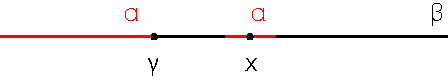
\includegraphics[width=0.6\textwidth ]{resources/part_set/ordinal1.pdf}  
	\caption{Relation of $\alpha$, $\beta$, $\gamma$ and $x$.}
	\label{fig:ordinal1}
\end{figure}

\begin{definition}
	Let $\alpha$ and $\beta$ be ordinals. We define $\alpha<\beta$ iff $\alpha\in\beta$.
\end{definition}
\begin{corollary}
	$<$ is a (strict) linear ordering of the class Ord.                                                                                                                                                                                                                                                                                                                                                                                                                                                                                                                                                                                                                                                                                                                                                                                                                                                                                                                                                                                                                                                                                                                                                                                                                                                                                                                                                                                                                                                                                                                                                                                                                                                                                                                                                                                                                                                                                                                                                                                                                                                                                                                                                                                                                                                                                                                                                                                                                                                                                                                                                                                                                                                                                                                                                                                                                                                                                                                                                                                              
\end{corollary}

\begin{lemma}
	If $C$ is a nonempty class of ordinals, then $\bigcap C$ is the least element of $C$. If $C$ is a nonempty set of ordinals, then $\bigcup C$ is the supremum of $C$.
\end{lemma}
\begin{corollary}
	Each set of ordinals has an upper bound in Ord.
\end{corollary}

\begin{lemma}
	Ord is a proper class.
\end{lemma}
\begin{proof}
	Otherwise, $Ord\in Ord$.
\end{proof}

\begin{lemma}
	Let $\alpha$ be an ordinal, $\alpha\cup\{\alpha\}$ is the least ordinal larger that $\alpha$.
\end{lemma}

\begin{definition}
	For each ordinal $\alpha$, we define $\alpha+1=\alpha\cup\{\alpha\}$.
\end{definition}

\begin{theorem}
	Every well-ordered set is isomorphic to a unique ordinal.\end{theorem}
\begin{proof}
	For each well-ordered set $X$. Let $X'=\{x\in X|\exists$ an ordinal $\alpha(X_{<x} $ is isomorphic to $\alpha)\}$. For each $x\in X'$, let $F(x)$ be the ordinal isomorphic to $X_{<x}$, which is unique due to Lem.\ref{lem:order_regular}. By the replacement axiom, $F(X')$ is a set. Let $\gamma$ be the least ordinal strictly larger than all of $F(X')$. If $X'\neq X$, let $x_0$ be the least element in $X-X'$. It's easy to see that $F$ is an isomorphism form $X_{<x_0}$ to $\gamma$. So $x_0\in X'$, a contradiction. So $X'=X$. It's easy to see that $F$ is an isomorphism form $X$ to $\gamma$.
\end{proof}
\begin{definition}
	The {\bf order type} of a well-ordered set is the ordinal it is isomorphic to.
\end{definition}

\section{Successor Ordinal and Limit Ordinal}
\begin{definition}
	If $\alpha=\beta+1$, then $\alpha$ is called a {\bf successor ordinal}. Otherwise $\alpha$ is called an {\bf limit ordinal}.
\end{definition}

\begin{lemma}
	There exists an inductive ordinal.
\end{lemma}
\begin{proof}
	Let $S$ be an inductive set. Let $S'=\{s\in S| s$ is an ordinal $\}$. $S'$ is nonempty since $\emptyset\in S'$. It's easy to see that $S'$ is inductive. Let $\alpha=\bigcup S'$. It's easy to see that $\alpha$ is an inductive ordinal.
\end{proof}

\begin{lemma}
	An ordinal is an inductive ordinal iff it's a nonzero limit ordinal.
\end{lemma}
\begin{proof}
	Let $\alpha$ be an inductive ordinal. If $\alpha=\beta+1$, then it's east to see $\alpha=\beta+1\in \alpha$, a contradiction.
	
	Let $\alpha$ be a nonzero limit ordinal. For each $\beta<\alpha$, $\beta+1<\alpha$.
\end{proof}

\begin{corollary}
	There exists a nonzero limit ordinal.
\end{corollary}

\begin{definition}
	We denote the least nonzero limit ordinal $\omega$(or $\mathbb N$). The ordinals less that $\omega$ (elements of $\mathbb N$) are called {\bf finite ordinals} or {\bf natural numbers}. The ordinals larger than or equal to $\omega$ are called {\bf infinite ordinals}. Specifically,
	\begin{equation}
		0=\emptyset,\ 1=0+1,\ 2=1+1,\ \dots
	\end{equation}
\end{definition}

\begin{lemma}
	Let $\alpha$ be an infinite ordinal, the order type of $\alpha\times\alpha$ with canonical order is $\alpha$.
	\label{lem:canorder}
\end{lemma}
\begin{proof}
	Let $\Gamma(\alpha)$ be the order type of $\alpha\times\alpha$. Clearly $\Gamma(\alpha)\geq\alpha$ and $\Gamma(\omega)=\omega$. Let $\beta$ be the least ordinal (if exists) in $\{\alpha|\Gamma(\alpha)>\alpha\}$. Let $f$ be the isomorphism $\beta\times\beta\mapsto \Gamma(\beta)$. It's easy to see that $f(\gamma,\gamma)=\Gamma(\gamma)=\gamma$ for each $\omega\leq\gamma<\beta$. So $f(\gamma,\gamma')\leq\max(\gamma,\gamma')<\beta$ for all $\omega\leq\gamma,\gamma'<\beta$. So $\Gamma(\beta)=f(\beta\times\beta)\leq \beta$, a contradiction.
\end{proof}

\begin{definition}
	A {\bf sequence} is a function $f$ whose domain is the set $\mathbb N$. An {\bf$\alpha$-sequence} is a function $f$ whose domain is an ordinal $\alpha$. $f(\beta)$ in a sequence is usually denoted by $f_\beta$. 
\end{definition}

\begin{definition}
	Let $a_\xi$ be a monotone $\alpha$-sequence. For each $\beta<\alpha$ define
	\begin{equation}
		\lim_{\xi\rightarrow\beta}=\sup\{a_\xi|\xi<\beta\}
	\end{equation}
\end{definition}

\section{Transfinite induction}

\begin{theorem}
	Let $C$ be a class of ordinals and assume that 
	\begin{enumerate}
		\item $0\in C$.
		\item $\alpha\in C$ implies that $\alpha+1\in C$.
		\item If $\alpha$ is a nonzero limit ordinal, $\beta\in C$ for all $\beta<\alpha$ implies that $\alpha\in C$.
	\end{enumerate}
	Then $C$ is the class of all ordinals.
\end{theorem}
\begin{proof}
	If not, consider the least ordinal not in $C$.
\end{proof}

\section{Ordinal Arithmetic}

\begin{definition}(Addition)
	For all ordinal number $\alpha$
	\begin{enumerate}
		\item $\alpha+0=\alpha$
		\item $\alpha+(\beta+1)=(\alpha+\beta)+1$ for each $\beta$
		\item $\alpha+\beta=\lim_{\gamma\rightarrow\beta}(\alpha+\gamma)$ for each limit $\beta$
	\end{enumerate}
\end{definition}

\begin{definition}(Multiplication)
	For all ordinal number $\alpha$
	\begin{enumerate}
		\item $\alpha\cdot 0=0$
		\item $\alpha\cdot(\beta+1)=\alpha\cdot\beta+1$ for each $\beta$
		\item $\alpha\cdot\beta=\lim_{\gamma\rightarrow\beta}(\alpha\cdot\gamma)$ for each limit $\beta$
	\end{enumerate}
\end{definition}

\begin{definition}(Exponentiation)
	For all ordinal number $\alpha$
	\begin{enumerate}
		\item $\alpha^0=1$
		\item $\alpha^{\beta+1}=\alpha^\beta\cdot \alpha$ for each $\beta$
		\item $\alpha^\beta=\lim_{\gamma\rightarrow\beta}\alpha^\gamma$ for each limit $\beta$
	\end{enumerate}
\end{definition}
\begin{lemma}
	\
	\begin{enumerate}
		\item $\forall\alpha\forall \beta\forall\gamma(\beta<\gamma\rightarrow\beta+\alpha<\gamma+\alpha )$
		\item $\forall\alpha\forall \beta(\alpha<\beta\rightarrow \exists !\gamma(\alpha+\gamma=\beta))$
		\item $\forall\alpha\forall \beta\forall\gamma(\alpha>0\wedge \beta<\gamma\rightarrow \alpha\cdot\beta<\alpha\cdot\gamma)$
		\item $\forall\alpha\forall\gamma(\alpha>0\rightarrow \exists !\beta\exists !$$\rho(\rho<\alpha\wedge \gamma=\alpha\cdot\beta+\rho))$
		\item $\forall\alpha\forall \beta\forall\gamma(\alpha>1\wedge \beta<\gamma\rightarrow \alpha^\beta<\alpha^\gamma)$
	\end{enumerate}
\end{lemma}
\begin{lemma}
	\
	\begin{enumerate}
		\item $\forall\alpha\forall \beta\forall\gamma(\alpha+(\beta+\gamma)=(\alpha+\beta)+\gamma)$ 
		\item $\forall\alpha\forall \beta\forall\gamma(\alpha\cdot(\beta\cdot\gamma)=(\alpha\cdot\beta)\cdot\gamma)$ 
	\end{enumerate}
\end{lemma}
\section{Cardinality and Uncountable Ordinal}

\begin{definition}
	Two sets $X,Y$ are called {\bf equipotent} if there's is a bijection map between them. 
\end{definition}
\begin{theorem}[Cantor-Bernstein]
	If there's an injective map from $X$ to $Y$, and there's also an injective map from $Y$ to $X$, then $X$ are $Y$ are equipotent.
\end{theorem}
\begin{proof}
	Let $f_1:X\mapsto Y$ and $f_2:Y\mapsto X$ be injective maps. We define by induction for all $n\in \mathbb N$:
	\begin{eqnarray}
		A_0&=&A\\
		A_{n+1}&=&f_2\circ f_1(A_n)\\
		B_0&=&f_2(B)\\
		B_{n+1}&=&f_2\circ f_1(B_n)
	\end{eqnarray}
	
	It's easy to see that $A_0\supseteq B_0\supseteq A_1\supseteq B_1\supseteq \cdots$.
	
	Define $g:X\mapsto Y$ as follows
	\begin{equation}
		g(x)=\left\{\begin{array}{ll}
			f_1(x)&x\in A_n-B_n {\rm\ for\ some\ } n\\
			f_2^{-1}(x)&{\rm otherwise}
		\end{array} \right.
	\end{equation}
	
	It's easy to see that $g$ is a bijection.
\end{proof}

\begin{corollary}
	Let $\alpha<\beta$ be two equipotent ordinals. Then for any $\gamma$ such that $\alpha\leq\gamma\leq\beta$, $\alpha$ is equipotent to $\gamma$.
\end{corollary}

\begin{lemma}
	Let $\alpha$ be an finite ordinal. Then $\alpha$ is the only ordinal that is equipotent to $\alpha$.
\end{lemma}
\begin{proof}
	It's easy to prove that for any finite ordinal $\alpha$, $\alpha$ is not equipotent to $\alpha+1$.

	For any finite ordinal $\alpha$, let $\beta$ any ordinal that is larger that $\alpha$ and is equipotent to $\alpha$. If such $\beta$ exists, clearly $\beta>\alpha+1>\alpha$. So $\alpha$ is equipotent to $\alpha+1$, a contradiction. So there's no ordinal lager than $\alpha$ that is equipotent to $\alpha$. Symmetrically, there's no ordinal smaller than $\alpha$ that is equipotent to $\alpha$.
\end{proof}

\begin{definition}
	A set is called {\bf finite} if it's equipotent to a finite ordinal, otherwise it's called {\bf infinite}. A set is called {\bf countable} if it's equipotent to $\omega$. A set is called {\bf at most countable} if it's finite or countable, otherwise it's called {\bf uncountable}.
\end{definition}

Sometimes we simply abbreviate ``at most countable" by ``countable".

\begin{theorem}[Hartogs]
	Let $\alpha$ be an ordinal, there's a least ordinal $\beta>\alpha$ and not equipotent to $\alpha$.
\end{theorem}
\begin{proof}
	Let $W$ be $\{$well orderings of $ a\subset\alpha\}$. $W$ is a set since it's a subset of $P(\alpha\times\alpha)$. Let $\beta$ be the set of order types of well-orderings in $W$.
	
	First we prove that $\beta$ is an ordinal $>\alpha$ and not equipotent to $\alpha$. For each $\gamma\in \beta$, let $f:b\mapsto\gamma$ be an isomorphism, where $b\subseteq\alpha$. For each $\delta\in \gamma$, $\delta\subset\gamma$. Then $f\cap f^{-1}(\delta)\times\delta$ is an isomorphism from $f^{-1}(\delta)$ to $\delta$. So $\delta\in \beta$. So $\beta$ is a transitive set of ordinals. So $\beta$ is an ordinal. Clearly $\beta>\alpha$. If $\beta$ is equipotent to $\alpha$, then $\beta$ induce a well-ordering on $\alpha$. Thus $\beta\in\beta$, a contradiction. 
	
	Next we prove that $\beta$ is the least ordinal with this property. For each $\gamma$ such that $\alpha<\gamma<\beta$, there's an injective map $\gamma\mapsto\alpha$ and an injective map $\alpha\mapsto\gamma$. So $\gamma$ and $\alpha$ are equipotent.
\end{proof}

\begin{corollary}
	There exists a least uncountable ordinal, denoted as $\omega_1$. We define $\Omega=\omega_1+1$
\end{corollary}


\chapter{Axiom of Regularity}
\begin{axiom}
	Every nonempty set $S$ has an element disjoint from $S$:
	\begin{equation}
		\forall S(S\neq \emptyset\rightarrow(\exists x\in S)S\cap x=\emptyset)
	\end{equation}
	
	This axiom can be reformulated as: every nonempty set has an $\in$-minimal element.
\end{axiom}

\begin{lemma}
	Let $S$ be a set. $S\not\in S$, and therefore $S\neq\{S\}$.
\end{lemma}
\begin{proof}
	Consider $\{S\}$.
\end{proof}
	
\begin{lemma}
	For every set $S$ there exists a smallest transitive set $TC(S)\supseteq S$ called the {\bf transitive closure} of $S$.
\end{lemma}
\begin{proof}
	We define by induction 
	\begin{equation}
		S_0=S,\ S_{n+1}=\bigcup S_n
	\end{equation}
	and let $TC(S)=\bigcup_n S_n$
\end{proof}

\begin{lemma}
	Every nonempty class $C$ has an $\in$-minimal element.
\end{lemma}
\begin{proof}
	Let $S\in C$ be arbitrary. If $S$ is not an $\in$-minimal element of $C$, $(\exists S'\in C)S'\in S$. Let $X=TC(S)\cap C$. Then $S'\in X\neq\emptyset$. By the axiom of regularity, there is $x\in X$ such that $x\cap X=\emptyset$. Since $x\subseteq TC(S)$, $x\subseteq TC(S)-C$. So $x\cap C=\emptyset$. Hence $x$ is a minimal element of $C$.
\end{proof}

\begin{corollary}
	It's impossible to have a sequence $S_i$ of sets such that $S_0\ni S_1\ni S_2\ni\cdots$.
\end{corollary}

\begin{definition}
	We define by induction that 
	\begin{eqnarray}
		V_0&=&\emptyset\\
		V_{\alpha+1}&=&P(V_\alpha)\\
		V_\alpha&=&\bigcup_{\beta<\alpha} V_\beta {\rm\ for\ limit\ }\alpha
	\end{eqnarray}
\end{definition}

For example
\begin{eqnarray}
	V_1&=&\{\emptyset\}=1\\
	V_2&=&\{\emptyset,\{\emptyset\}\}=2\\
	V_3&=&\{\emptyset,\{\emptyset\},\{\{\emptyset\}\},\{\emptyset,\{\emptyset\}\}\}=3\cup\{\{1\}\}
\end{eqnarray}

\begin{lemma}
	\
	\begin{enumerate}
		\item Each $V_\alpha$ is transitive.
		\item $\alpha<\beta\rightarrow V_\alpha\subseteq V_\beta$.
		\item $\alpha\subseteq V_\alpha$.
	\end{enumerate}
\end{lemma}

\begin{lemma}
	For every $x$ there is $\alpha$ such that $x\in V_\alpha$
\end{lemma}
\begin{proof}
	Let $C$ be the class of $x$ that are not in any $V_\alpha$. If $C$ is nonempty, then $C$ has an $\in$-minimal element $x$	. For each $t$ in some $V_\alpha$, we define $rank(t)=\inf\{\alpha|t\in V_\alpha\}$. Then $rank(x)$ is a set of ordinals, with supremum $\lambda$. It's easy to see that $x\subseteq V_\lambda$. So $x\in V_{\lambda+1}$. Thus $C$ is empty.
\end{proof}

\begin{definition}
	For each set $x$, we define the {\bf rank} of $x$ to be $\inf\{\alpha|x\in V_\alpha\}$.
\end{definition}

\chapter{Axiom of Choice}

\begin{axiom}
	Every family $S$ of nonempty sets has a choice function $S\mapsto \bigsqcup S$:
	\begin{equation}
		\forall X\in S(f(X)\in X)
	\end{equation}
\end{axiom}

\begin{lemma}
	Let $A$ be a set and $F$ be a choice function on nonempty subsets of $A$.	
	If
	\begin{enumerate}
		\item We have $X_0\neq\emptyset$ 
		\item $f(\alpha)$ is defined as $f(\alpha)=F(X_\alpha)$ if $X_\alpha\neq\emptyset$
		\item $X_\alpha$ is defined by a definitive rule if $f(\beta)$ is defined and $\not\in X_\alpha$ for $\beta<\alpha$.
	\end{enumerate}
	We can define by induction $X_\alpha\in A$ for $\alpha\leq\theta$, and $f(\alpha)$ for $\alpha<\theta$, where $X_\theta=\emptyset$, and $f$ is injective.
	
	\label{lem:choice}
\end{lemma}
\begin{proof}
	If such $\theta$ doesn't exist, $Ord$ would be a subset of $A$.
\end{proof}

\begin{theorem}
	The axiom of choice is equivalent to
	\begin{enumerate}
		\item[] {\bf Well-ordering principle:} Every set can be well-ordered.
		\item[] {\bf Zorn's lemma:} A nonempty partially ordered set in which every chain has an upper bound has a maximal element.
	\end{enumerate}
\end{theorem}
\begin{proof}
	\

	{\bf Axiom of choice $\rightarrow$ Well-ordering principle:}

	Let $A$ be a nonempty set, and $F$ be a choice function on nonempty subsets of $A$. We define a function $f$ as $f(\alpha)=F(A-\{f(\beta)|\beta<\alpha\})$ if $A\neq \{f(\beta)|\beta<\alpha\}$. By Lem.\ref{lem:choice}, there exists an $\alpha$ such that $f:\alpha\mapsto A$ and $A=\{f(\beta)|\beta<\alpha\}$. It's easy to see that $f$ is bijective. So $A$ can be well-ordered according to the well-ordering on $\alpha$.

	{\bf Well-ordering principle $\rightarrow$ Axiom of choice:}

	We well-order $\bigcup S$ and define $f(X)=\inf\{x\in\bigcup S|x\in X\}$.

	{\bf Axiom of choice $\rightarrow$ Zorn's lemma:}
	
	Let $P$ be a nonempty partially ordered set. Let $F$ be a choice function on nonempty subsets of $P$. We define a function $f$ as $f(\alpha)=F(\{p\in P|(\forall\beta<\alpha)p>f(\beta)\})$ if $(\exists p\in P)(\forall\beta<\alpha)p>f(\beta)$. By Lem.\ref{lem:choice}, there exists an $\alpha$ such that $f:\alpha\mapsto P$ and $(\not\exists p\in P)(\forall\beta<\alpha)p>f(\beta)$. $\{f(\beta)|\beta<\alpha\}$ is a chain in $P$, with an upper bound $q$. It's easy to see that $q$ is the maximal element in $P$.

	{\bf Zorn's lemma $\rightarrow$ Axiom of choice:}
	
	Let $S$ be a family of sets, and $P=\{f| f$ is a choice function on some $Z\subseteq S\}$. $P$ is partially ordered by $\subseteq$. For each chain $P'$ in $P$, it's easy to see that $\bigcup P'\in P$ is the upper bound of $P'$. Use the Zorn's lemma, $P$ has a maximal element $F$. It's easy to see that $F$ is a choice function on $S$.
\end{proof}

\chapter{Cardinal Numbers}

\begin{definition}
	An ordinal $\alpha$ is called a {\bf cardinal number} if $\alpha$ is not isomorphic to $\beta$ for all $\beta<\alpha$.
\end{definition}

\begin{definition}
	For each set $X$, $|X|$ is defined to be the least ordinal that $X$ is equipotent to. Clearly $|X|$ is a cardinal number. $|X|$ is well-defined since $X$ can be well-ordered.
\end{definition}
\begin{lemma}
	$X$ are $Y$ are equipotent iff $|X|=|Y|$. There is an injective map from $X$ to $Y$ iff $|X|\leq|Y|$.
\end{lemma}

\begin{lemma}
	$|X|<|P(X)|$.
\end{lemma}
\begin{proof}
	If not, let $f:X\mapsto P(X)$ be a bijection. Let $Y=\{x\in X|x\not\in f(x)\}$. $Y\not\in f(X)$.
\end{proof}

\begin{lemma}
	For each cardinal $\alpha$, there's a cardinal strictly larger than $\alpha$.
\end{lemma}

\begin{definition}
	For each ordinal $\alpha$, we define $\alpha^+$ to be the least cardinal strictly larger than $\alpha$.
\end{definition}

\begin{lemma}
	Let $X$ be a set of cardinals, then $\sup X$(in Ord) is a cardinal.
\end{lemma}

\section{Finite and Infinite Cardinals}

\begin{definition}
	A cardinal is called a {\bf finite cardinal} iff it's a finite ordinal. A cardinal is called an {\bf infinite cardinal} iff it's a infinite ordinal.
\end{definition}

\begin{lemma}
	Let $\alpha$ be an ordinal, then $|\alpha|=|\alpha+1|$ iff $\alpha$ is infinite.
\end{lemma}
\begin{proof}
	If $\alpha$ is infinite, the injective map $f:(\alpha+1)\mapsto\alpha$ is defined as
	\begin{eqnarray}
		f(\alpha)&=&0\\
		f(\beta)&=&\beta+1\ (\beta<\alpha)
	\end{eqnarray}
\end{proof}

\begin{corollary}
	Each finite ordinal is a finite cardinal. Each infinite cardinal is a limit ordinal. 
\end{corollary}

\begin{definition}
	We define 
	\begin{eqnarray}
		&&\aleph_0=\omega_0=\omega\\
		&&\aleph_{\alpha+1}=\omega_{\alpha+1}=\aleph_\alpha^+\\
		&&\aleph_\alpha=\omega_\alpha=\sup\{\omega_\beta|\beta<\alpha\}{\rm\ if\ } \alpha {\rm\ is\ a\ limit\ ordinal}
	\end{eqnarray}
	
	We usually use $\aleph_\alpha$ to refer to cardinal numbers, and use $\omega_\alpha$ to refer to ordinal numbers.  
\end{definition}
\begin{lemma}
	$\alpha<\beta\leftrightarrow \aleph_\alpha<\aleph_\beta$.
\end{lemma}

\begin{lemma}
	Each infinite cardinal number is some $\aleph_\alpha$.
\end{lemma}
\begin{proof}
	It's easy to see that $\aleph_\alpha\geq\alpha$ for each $\alpha$, since $\alpha\rightarrow\aleph_\alpha$ is a morphism in {\bf Poset}. So $\forall$ cardinal $\kappa \exists $ ordinal $\alpha(\aleph_\alpha>\kappa)$. Let $\gamma=\inf\{\beta|\aleph_\beta\geq\kappa\}$. Then it's easy to see that $\kappa=\aleph_\gamma$.
\end{proof}

\begin{definition}
	An infinite cardinal $\aleph_\alpha$ is called a {\bf successor cardinal} iff $\alpha$ is a successor ordinal. An infinite cardinal $\aleph_\alpha$ is called a {\bf limit cardinal} iff $\alpha$ is a limit ordinal.
\end{definition}

\section{Cardinal Arithmetic}
\begin{definition}
	Let $|A|=\kappa$ and $B=\lambda$. We define
	\begin{enumerate}
		\item $\kappa+\lambda=|A\sqcup B|$.
		\item $\kappa\cdot\lambda=|A\times B|$.
		\item $\kappa^\lambda=|A^B|$.
	\end{enumerate}
\end{definition}

Note that the cardinal numbers have the same order but (possibly) different arithmetic with the ordinal numbers.

\begin{theorem}
	\begin{equation}
		\aleph_\alpha\cdot\aleph_\alpha=\aleph_\alpha
	\end{equation}
\end{theorem}
\begin{proof}
	Clearly $\aleph_\alpha\leq\aleph_\alpha\cdot\aleph_\alpha$. From Lem.\ref{lem:canorder}, we have $\aleph_\alpha\cdot\aleph_\alpha\leq\aleph_\alpha$.
\end{proof}
\begin{corollary}
	Let $\kappa$ and $\lambda$ be two non-zero cardinals, one of which is infinite. Then $\kappa+\lambda=\kappa\cdot\lambda=\max\{\kappa,\lambda\}$
\end{corollary}
\begin{proof}
	$\max\{\kappa,\lambda\}\leq\kappa+\lambda\leq\kappa\cdot\lambda\leq\max\{\kappa,\lambda\}\cdot\max\{\kappa,\lambda\}=\max\{\kappa,\lambda\}$
\end{proof}

\begin{definition}
	Let $\{\kappa_i|i\in I\}$ be an indexed set of cardinal numbers. We define
	\begin{equation}
		\sum_{i\in I}\kappa_i=\Big|\bigsqcup_{i\in I}\kappa_i\Big|
	\end{equation}
\end{definition}

\begin{lemma}
	Let $\{\kappa_i|i\in I\}$ be an indexed set of cardinal numbers, and $|I|$ or $\sup\{\kappa_i\}$ be infinite. Then
	\begin{equation}
		\sum_{i\in I}\kappa_i=|I|\cdot \sup\{\kappa_i\}
	\end{equation}
\end{lemma}
\begin{proof}
	Note that $\sup\{\kappa_i\}$ is a cardinal. It's easy to see that there's a injective map from $\sum_{i\in I}\kappa_i$ to $|I|\cdot \sup\{\kappa_i\}$. On the other hand, it's easy to see that $|I|\leq\sum_{i\in I}\kappa_i$ and $\sup\{\kappa_i\}\leq \sum_{i\in I}\kappa_i$ (since $\forall i(\kappa_i\leq \sum_{i\in I}\kappa_i)$).
\end{proof}

\begin{lemma}
	Let $\{\kappa_{ij}|i\in I, j\in J_i\}$ be an indexed set of ordinal numbers. 
	\begin{equation}
		\sup\{\sup\{ \kappa_{ij}|j\in J_i\}|i\in I\}=\sup\{ \kappa_{ij}|i\in I,j\in J_i\}
	\end{equation}
	\label{lem:inf_sum_lim}
\end{lemma}

\begin{lemma}
	Let $\kappa_\lambda$ be an $\alpha$-sequence, where $\alpha$ is a infinite cardinal. Then $\sum_{\lambda<\alpha}\kappa_\lambda=\lim_{\beta\rightarrow\alpha}\sum_{\lambda\leq\beta}\kappa_\lambda$.
\end{lemma}
\begin{proof}
	$\lim_{\beta\rightarrow\alpha}\sum_{\lambda\leq\beta}\kappa_\lambda=\lim_{\beta\rightarrow\alpha}(|\beta|\cdot\sup\{|\kappa_\lambda||\lambda\leq\beta\})=\max(\alpha,\sup\{|\kappa_\lambda||\lambda<\alpha\})=\sum_{\lambda<\alpha}\kappa_\lambda$.
\end{proof}

\begin{lemma}
	$|P(X)|=2^{|X|}$
\end{lemma}
\begin{corollary}
	$\kappa<2^\kappa$, $\kappa^+\leq 2^\kappa$
\end{corollary}

\begin{lemma}
	\
	\begin{enumerate}
		\item $(\kappa^\lambda)^\theta=\kappa^{\lambda\cdot\theta}$
		\item $\kappa^\lambda\cdot\kappa^\theta=\kappa^{\lambda+\theta}$
		\item $\lambda>\theta\rightarrow \kappa^\lambda\geq\kappa^\theta$
		\item $\lambda>\theta\rightarrow \lambda^\kappa\geq\theta^\kappa$
	\end{enumerate}
\end{lemma}

\begin{lemma}
	If $2\leq\kappa\leq\lambda$ and $\lambda$ is infinite, then $\kappa^\lambda=2^\lambda$.
\end{lemma}
\begin{proof}
	\begin{equation}
		2^\lambda\leq \kappa^\lambda\leq(2^\kappa)^\lambda=2^{\kappa\cdot\lambda}=2^\lambda
	\end{equation}
\end{proof}

\section{Cofinality}

\begin{definition}
	A function $A\mapsto B$ between two pre-ordered set is called {\bf cofinal} in $\beta$ iff 
	\begin{equation}
		\forall \beta\in B\exists \alpha\in A(f(\alpha)\geq\beta)
	\end{equation}
\end{definition}

\begin{definition}
	Let $\alpha>0$ be a limit ordinal. We define $cf(\alpha)$ to be the least $\beta$ such that there's a cofinal map $\beta\mapsto\alpha$.
\end{definition}

$cf(\alpha)$ is the least ordinal that resembles the interval $(\alpha-\epsilon,\alpha)$.

\begin{lemma}
	\
	\begin{enumerate}
		\item $cf(\alpha)$ is a limit ordinal.
		\item $cf(\alpha)\leq \alpha$.
		\item $cf(cf(\alpha))=cf(\alpha)$
	\end{enumerate}
\end{lemma}
\begin{proof}
	3. The composition of cofinal functions is cofinal.
\end{proof}

\begin{definition}
	Let $\alpha>0$ be a limit ordinal. $\alpha$ is called {\bf regular} if $cf(\alpha)=\alpha$. Otherwise $\alpha$ is called {\bf singular}.
\end{definition}

\begin{lemma}
	Let $\alpha>0$ be a limit ordinal. $cf(\alpha)$ is a regular cardinal.
\end{lemma}

\begin{lemma}
	Let $\alpha,\beta$ be infinite cardinals. There's a cofinal function $f:\alpha\mapsto\beta$ iff there is a function $g:\alpha\mapsto\beta$ such that $\sum_{\theta<\alpha} g(\theta)=\beta$.
\end{lemma}
\begin{proof}
	Let $f:\alpha\mapsto\beta$ be cofinal, define
	\begin{equation}
		g(\theta)=\left\{\begin{array}{cc}
			f(0)&\alpha=0\\
			\bigcup_{\beta\leq\theta+1} f(\beta)-\bigcup_{\beta\leq\theta} f(\beta) &\theta>0
		\end{array} \right.
	\end{equation}
	Clearly $\sum_{\theta<\alpha} g(\theta)=|\bigsqcup_{\theta<\alpha} g(\theta)|=|\bigcup_{\theta<\alpha} f(\theta)|=\beta$.
	
	Let $g:\alpha\mapsto\beta$ be a function such that $\sum_{\theta<\alpha} g(\theta)=\beta$. We define $f(\theta)=\sum_{\lambda\leq\theta}g(\lambda)$. From Lem. \ref{lem:inf_sum_lim}, we have $\sup\{f(\theta)|\theta<\alpha\}=\beta$. So $f$ is cofinal.
\end{proof}

\begin{corollary}
	Let $\kappa$ be an infinite cardinal. $cf(\kappa)=\inf\{\theta\in Ord|\exists$ a $\theta$-sequence $\kappa_\nu$ of cardinals $\kappa_\nu<\kappa$ with $\kappa=\sum_{\nu<\theta}\kappa_\nu\}$. 
\end{corollary}

\begin{corollary}
	An infinite successor cardinal is regular.
\end{corollary}
\begin{proof}
	Let $\kappa$ be an infinite cardinal. There exists a $cf(\kappa^+)$-sequence $\kappa_\nu$ of cardinals $\kappa_\nu<\kappa^+$ with $\kappa^+=\sum_{\nu<cf(\kappa^+)}\kappa_\nu=\max(cf(\kappa^+),\sup\{\kappa_\nu\})$. Since $\kappa_\nu<\kappa^+$, $\kappa_\nu\leq\kappa$. So $\sup\{\kappa_\nu\}\leq\kappa<\kappa^+$.  We must have $cf(\kappa^+)=\kappa^+$.
\end{proof}

The classification of cardinal numbers is shown in Fig. \ref{fig:cardinal1}.

\begin{figure}[htb!]
	\centering  
	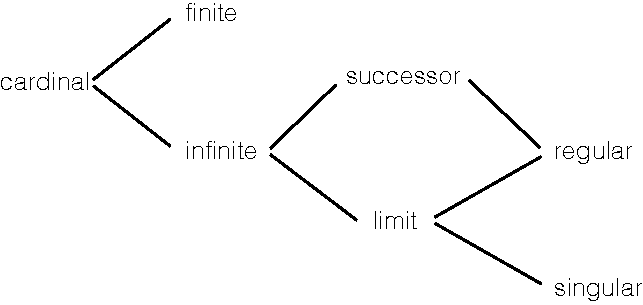
\includegraphics[width=0.7\textwidth ]{resources/part_set/cardinal1.pdf}  
	\caption{Classification of cardinal numbers.}
	\label{fig:cardinal1}
\end{figure}

\section{Cardinal Exponentiation}

\begin{theorem}[K\"onig]
	If $\kappa$ is an infinite cardinal, then $\kappa<\kappa^{cf(\kappa)}$.
\end{theorem}
\begin{proof}
	It's easy to see that $\kappa\leq\kappa^{cf(\kappa)}$. If $\kappa=\kappa^{cf(\kappa)}$, let $f$ be the bijection between them. Let $g$ be a cofinal map $cf(\kappa)\mapsto\kappa$. Define $h:cf(\kappa)\mapsto\kappa$ as
	\begin{equation}
		h(\xi)=\inf(\kappa- \{f(\alpha)(\xi)|\alpha<g(\xi)\})
	\end{equation}
	$h(\xi)$ is well-defined since $|\{f(\alpha)(\xi)|\alpha<g(\xi)\}|\leq|g(\xi)|<\kappa$. $h\not\in f(\kappa)$ since $\forall \alpha\exists\xi (h(\xi)\neq f(\alpha)(\xi))$.
\end{proof}

\begin{lemma}
	Let $\kappa$ be an infinite cardinal and $\lambda<cf(\kappa)$. Then
	\begin{equation}
		\kappa^\lambda=\kappa\cdot\sup_{\theta<\kappa}\theta^\lambda
	\end{equation}
	\label{lem:kappa_exp}
\end{lemma}
\begin{proof}
	If $\lambda<cf(\kappa)$, $(\forall f:\lambda\mapsto\kappa)\exists(\theta<\kappa)f(\kappa)\subseteq \theta$. So $\kappa^\lambda=|\cup_{\alpha<\kappa}\alpha^\lambda|\leq |\sqcup_{\alpha<\kappa}\alpha^\lambda|=|\sqcup_{\alpha<\kappa}|\alpha|^\lambda|=\sum_{\alpha<\kappa}|\alpha|^\lambda=\kappa\cdot\sup_{\theta<\kappa}\theta^\lambda$ where $\alpha$ are ordinals and $\theta$ are cardinals. On the other hand $\kappa\leq\kappa^\lambda$ and $\sup_{\theta<\kappa}\theta^\lambda\leq\kappa^\lambda$.
\end{proof}

\begin{corollary}
	We have the {\bf Hausdorff formula} $\aleph_{\alpha+1}^{\aleph_\beta}=\aleph_{\alpha+1}\cdot\aleph_{\alpha}^{\aleph_\beta}$ for all $\alpha$ and $\beta$.
\end{corollary}
\begin{proof}
	
	When $\beta\leq\alpha$, use Lem.\ref{lem:kappa_exp}. When $\beta>\alpha$, the Hausdorff formula holds because $\aleph_{\alpha+1}^{\aleph_\beta}=\aleph_{\alpha}^{\aleph_\beta}=2^{\aleph_\beta}>\aleph_{\alpha+1}$.
\end{proof}

\begin{theorem}
	Let $\lambda$ be an infinite ordinal. Then for all infinite cardinals $\kappa$,
	\begin{enumerate}
		\item if $\kappa\leq\lambda$ then $\kappa^\lambda=2^\lambda$,
		\item if there exists some $\mu<\kappa$ such that $\mu^\lambda\geq\kappa$, then $\kappa^\lambda=\mu^\lambda$,
		\item if $\kappa>\lambda$ and $\mu^\lambda<\kappa$ for all $\mu<\kappa$, then
		\item[] \begin{enumerate}
					\item[a.] $\kappa^\lambda=\kappa$ if $cf(\kappa)>\lambda$,
					\item[b.] $\kappa^\lambda=\kappa^{cf(\kappa)}$ if $cf(\kappa)\leq\lambda$.
				\end{enumerate}
	\end{enumerate}
\end{theorem}
\begin{proof}
	In the case 3, using the assumption, we have $\sup_{\alpha<\kappa}|\alpha|^\lambda= \kappa$

	In the case 3.a: $\kappa^\lambda=\max(\kappa,\sup_{\alpha<\kappa}|\alpha|^\lambda)=\kappa$.
	
	In the case 3.b: $\kappa$ must be a limit cardinal. It's easy to see that $\kappa^\lambda\geq\kappa^{cf(\kappa)}$. We only need to prove that $\kappa^\lambda\leq\kappa^{cf(\kappa)}$. Let $h:cf(\kappa)\mapsto \kappa$ be a cofinal map. To each $f:\lambda\mapsto\kappa$ and each $\beta<cf(\kappa)$ we associate a function $f_\beta:\lambda\mapsto\kappa:$
	\begin{equation}
		f_\beta(\alpha)=\min(f(\alpha),h(\beta))
	\end{equation}
	The map $f\mapsto (f_\beta)$ is a injective map from $\kappa^\lambda$ to $(\bigcup_{\alpha<\kappa}\alpha^\lambda)^{cf(\kappa)}$. So $\kappa^\lambda\leq|\bigcup_{\alpha<\kappa}\alpha^\lambda|^{cf(\kappa)}=\kappa^{cf(\kappa)}$. Since $\kappa\leq|\bigcup_{\alpha<\kappa}\alpha^\lambda|\leq|\bigsqcup_{\alpha<\kappa}\alpha^\lambda|=\max(\kappa,\sup_{\alpha<\kappa}|\alpha|^\lambda)=\kappa$.
\end{proof}
\section{Continuum Hypothesis}
\begin{axiom}
	The {\bf continuum hypothesis} is the statement $2^{\aleph_0}=\aleph_1$.
\end{axiom}
\begin{axiom}
	The {\bf generalized continuum hypothesis}(GCH) is the statement $2^{\aleph_\alpha}=\aleph_{\alpha+1}$.
\end{axiom}

\begin{theorem}
	If GCH holds and $\kappa$ and $\lambda$ are infinite cardinals, then
	\begin{enumerate}
		\item if $\kappa\leq\lambda$ then $\kappa^\lambda=\lambda^+$,
		\item if $cf(\kappa)\leq\lambda<\kappa$ then $\kappa^\lambda=\kappa^+$,
		\item if $\lambda<cf(\kappa)$ then $\kappa^\lambda=\kappa$.
	\end{enumerate}
\end{theorem}
\begin{proof}
	When $\lambda<\kappa$, $\kappa\leq \kappa^\lambda\leq (2^\kappa)^\lambda=2^\kappa=\kappa^+$. If $cf(\kappa)\leq\lambda$, then $\kappa<\kappa^{cf(\kappa)}\leq \kappa^\lambda$. So $\kappa^\lambda=\kappa^+$. If $\lambda<cf(\kappa)$, then $\kappa^\lambda=\kappa\cdot\sup\{|\alpha|^\lambda|\alpha<\kappa\}\leq\kappa\cdot\sup\{(2^{|\alpha|})^\lambda|\alpha<\kappa\}=\kappa\cdot\sup\{(|\alpha|\cdot\lambda)^+|\alpha<\kappa\}=\kappa$.
\end{proof}
\part{General topology}
\chapter{Topological Space}
	
\begin{definition}
	Let $X$ be a set and $\mathcal T$ be a family of subsets of $X$. $(X,\mathcal T)$ is called a {\bf topological space} if
	\begin{enumerate}
		\item[O1] any union of elements in $\mathcal T$ belongs to $\mathcal T$.
		\item[O2] any finite intersection of elements in $\mathcal T$ belongs to $\mathcal T$.
		\item[O3] $\emptyset$ and $X$ belong to $\mathcal T$.
	\end{enumerate}
	
	Elements of $\mathcal T$ are called {\bf open subsets} of $X$. We also call $\mathcal T$ a topology on $X$, and call $(X,\mathcal T)$ $X$ with topology $\mathcal T$.
\end{definition}

\begin{definition}
	Let $\mathcal T_1$ and $\mathcal T_2$ be two topologies on $X$. $\mathcal T_1$ is called {\bf finer(stronger)} than $\mathcal T_2$ if $\mathcal T_1\supseteq \mathcal T_2$. $\mathcal T_1$ is called {\bf coarser(weaker)} than $\mathcal T_2$ if $\mathcal T_1\subseteq \mathcal T_2$.
\end{definition}

\begin{definition}
	Let $(X,\mathcal T)$ be a topological space, and $S$ be a subset of $X$. $S$ is called {\bf closed} if $X-S$ (denoted by $S^\neg$) is open. 
\end{definition}

\begin{lemma}
	Let $\mathcal F$ be the family of closed subsets of $X$. Then
	\begin{enumerate}
		\item[C1] any finite union of elements in $\mathcal F$ belongs to $\mathcal F$,
		\item[C2] any intersection of elements in $\mathcal F$ belongs to $\mathcal F$,
		\item[C3] $\emptyset$ and $X$ belong to $\mathcal F$,
	\end{enumerate}
	and furthermore
	\begin{enumerate}
		\item[C4] $S\subseteq X$ is open if $S^\neg$ is closed.
	\end{enumerate}

	Let $\mathcal F$ be a family of subsets of $X$ that satisfies C1-C3. Then $\mathcal F$ is the family of closed subsets of a topology space, whose open sets are defined by C4.
\end{lemma}

\section{Base and subbase}

\begin{definition}
	Let $(X,\mathcal T)$ be a topological space, and $\mathcal B$ be a subfamily of $\mathcal T$. $\mathcal B$ is called a {\bf base} if $(\forall x\in X)(\forall  S\in \mathcal T)x\in S\rightarrow(\exists B\in \mathcal B)x\in B\subseteq S$. 
\end{definition}

\begin{lemma}
	Let $X$ be a set and $\mathcal B$ be a base of $(X,\mathcal T)$. Then
	\begin{enumerate}
		\item[B1] $(\forall x\in X)(\exists B\in \mathcal B)x\in B$
		\item[B2] $(\forall B_1,B_2\in \mathcal B)(\forall x\in B_1\cap B_2)(\exists B_3\in \mathcal B)x\in B_3\subseteq B_1\cap B_2$
	\end{enumerate}
	and furthermore
	\begin{enumerate}
		\item[B3] $S\subseteq X$ is open if $(\forall x\in S)(\exists B\in \mathcal B)x\in B\subseteq S$.
	\end{enumerate}
	
	Let $\mathcal B$ be a family of subsets of $X$ that satisfies B1 and B2. Then $\mathcal B$ is the base of a topology space, and open sets are defined by B3.
\end{lemma}

\begin{definition}
	Let $(X,\mathcal T)$ be a topological space, and $\mathcal B_x$ be a subfamily of $\mathcal T$ that contains $x$. $\mathcal B_x$ is called a {\bf local base} at $x$ if $(\forall S\in \mathcal T)x\in S \rightarrow(\exists B\in \mathcal B_x)x\in B\subseteq S$. 
\end{definition}

\begin{lemma}
	Let $(X,\mathcal T)$ be a topological space, and for each $x$, $\mathcal B_x$ be a local base at $x$. Then
	\begin{enumerate}
		\item [LB1] $(\forall B\in \mathcal B_x)x\in B$,
		\item [LB2] $(\forall B_1,B_2\in \mathcal B_x)(\exists B_3\in \mathcal B_x) B_3\subseteq B_1\cap B_2$,
		\item [LB3] $(\forall B\in \mathcal B_x )(\forall y\in B )(\exists B'\in \mathcal B_y)B'\subseteq B$.
	\end{enumerate}
	and furthermore
	\begin{enumerate}
		\item[LB4] $S\subseteq X$ is open if $(\forall x\in S)(\exists B\in \mathcal B_x)x\in B_x\subseteq S$.
	\end{enumerate}
	
	$\forall x\in X$ let $\mathcal B_x$ be a family of subsets of $X$ that satisfies LB1-LB3. Then $\mathcal B_x$ is the local base of a topology space, and open sets are defined by LB4.
\end{lemma}

\begin{lemma}
	Let $(X,\mathcal T)$ be a topological space. If $\forall x\in X$ we have a local base $\mathcal B_x$, then $\bigcup_{x\in X}\mathcal B_x$ is a base.
\end{lemma}

\begin{definition}
	Let $(X,\mathcal T)$ be a topological space, and $\mathcal S$ be a subfamily of $\mathcal T$. $\mathcal S$ is called a {\bf subbase} if the collection of all finite intersections of $\mathcal S$ is a base.
\end{definition}

\begin{lemma}
	Let $X$ be a set and $\mathcal S$ be a family of subsets of $X$. $\mathcal S$ is a subbase for a topology on $X$ with the collection of all finite intersections of $\mathcal S$ as its base.
\end{lemma}

\section{Neighborhoods}

\begin{definition}
	Let $(X,\mathcal T)$ be a topological space, $x\in X$ and $S\subseteq X$. $S$ is called the {\bf neighborhood} at $x$ if $\exists A\in \mathcal T: x\in A\subseteq S$. The family of neighborhoods at $x$ is called the neighborhood system at $x$, denoted by $\mathcal N_x$.
\end{definition}

\begin{theorem}
	Let $(X,\mathcal T)$ be a topological space, and $\forall x\in X$, $\mathcal N_x$ be a neighborhood system at $x$. Then
	\begin{enumerate}
		\item [N1] $\forall N\in \mathcal N_x:x\in N$,
		\item [N2] $\forall N_1,N_2\in \mathcal N_x: N_1\cap N_2\in \mathcal N_x$,
		\item [N3] $\forall N\in \mathcal N_x\exists N'\in \mathcal N_x\forall y\in N':N\in \mathcal N_y$.
		\item [N4] $\forall N\in \mathcal N_x:N\subseteq N'\Rightarrow N'\in \mathcal N_x$,
	\end{enumerate}
	and furthermore
	\begin{enumerate}
		\item[N5] $S\subseteq X$ is open if $\forall x\in S\exists N\in \mathcal N_x:x\in N_x\subseteq S$.
	\end{enumerate}
	
	$\forall x\in X$ let $\mathcal N_x$ be a family of subsets of $X$ that satisfies N1-N4. Then $\mathcal N_x$ is the neighborhood system of a topology space, and open sets are defined by N5.
\end{theorem}

\begin{definition}
	Let $(X,\mathcal T)$ be a topological space, $\mathcal {NB}_x$ be a subfamily of $\mathcal N_x$. $\mathcal {NB}_x$ is called the {\bf neighborhood base} at $x$ if $\forall A\in \mathcal T:x\in A\exists B\in \mathcal {NB}_x: x\in B\subseteq A$. Elements of a neighborhood base are called {\bf basic neighborhoods}.
\end{definition}

\begin{theorem}
	Let $(X,\mathcal T)$ be a topological space. A local base at $x\in X$ is a neighborhood base.
\end{theorem}

\begin{theorem}
	Let $(X,\mathcal T)$ be a topological space, and $\forall x\in X:\mathcal {NB}_x$ be a neighborhood base at $x$. Then
	\begin{enumerate}
		\item [NB1] $\forall N\in \mathcal {NB}_x:x\in N$,
		\item [NB2] $\forall N_1,N_2\in \mathcal {NB}_x\exists N_3\in \mathcal {NB}_x: N_3\subseteq N_1\cap N_2$,
		\item [NB3] $\forall N\in \mathcal {NB}_x\exists N'\subseteq N\forall y\in N'\exists N''\in \mathcal {NB}_y:N''\subseteq N$.
	\end{enumerate}
	and furthermore
	\begin{enumerate}
		\item[NB4] $S\subseteq X$ is open if $\forall x\in S\exists N\in \mathcal{NB}_x:x\in N_x\subseteq S$.
	\end{enumerate}
	
	$\forall x\in X$ let $\mathcal {NB}_x$ be a family of subsets of $X$ that satisfies NB1-NB3. Then $\mathcal {NB}_x$ is the neighborhood base of a topology space, and open sets are defined by NB4.
\end{theorem}

\begin{theorem}
	Let $(X,\mathcal T)$ be a topological space, $E\subseteq X$ Then
	\begin{enumerate}
		\item $E$ is open iff $E$ contains a basic neighborhood of each of its points.
		\item $E$ is closed iff each $x\not\in E$ has a basic neighborhood disjoint from $E$.
		\item $E^-=\{x\in X|$ each basic neighborhood of $x$ meets $E\}$
		\item $E^\circ=\{x\in X|$ some basic neighborhood of $x$ is contained in $E\}$
	\end{enumerate}
\end{theorem}


\section{Closure and Interior}

\begin{definition}
	Let $(X,\mathcal T)$ be a topological space and $S\subseteq X$. The {\bf closure} of $S$, denoted by $S^-$ or $Cl_X(S)$, is defined to be the intersection of all closed subsets that contains $S$. The {\bf interior} of $S$, denoted by $S^\circ$ or $Int_X(S)$, is defined to be the union of all open subsets that is contained in $S$. The {\bf frontier} of $S$, denoted by $Fr_X(S)$, is defined to be $S^--S^\circ$. The {\bf boundary} of $S$, denoted by $\partial_X(S)$, is defined to be $S-S^\circ$.
\end{definition}

\begin{lemma}
	Let $A$ and $B$ be subsets of topological space $X$
	\begin{eqnarray}
		A\subseteq B&\Rightarrow& A^-\subseteq B^- \wedge A^\circ\subseteq B^\circ\\
		A^{\circ}&=&A^{\neg -\neg}\\
		A^{\circ-}&=&A^{\circ-\circ-}\\
		A^{-\circ}&=&A^{-\circ-\circ}\\
		(A\cup B)^-&=&A^-\cup B^-\\
		(A\cap B)^\circ&=&A^\circ\cap B^\circ
	\end{eqnarray}
	where $\neg$ denotes complementation.
\end{lemma}
\begin{proof}
	Since for any closed $S$ we have $S^{\circ-}\subseteq S$, we have $A^{\circ-\circ-}\subseteq A^{\circ-}$. Since for any open $S$ we have $S\subseteq S^{-\circ}$, we have $A^{\circ}\subseteq A^{\circ-\circ}$. So $A^{\circ-}\subseteq A^{\circ-\circ-}$. So $A^{\circ-}=A^{\circ-\circ-}$. Similarly $A^{-\circ}=A^{-\circ-\circ}$.
\end{proof}

The concepts of closure, interior and frontier are illustrated in Fig. \ref{fig:topospace1}.

\begin{figure}[htb!]
	\centering  
	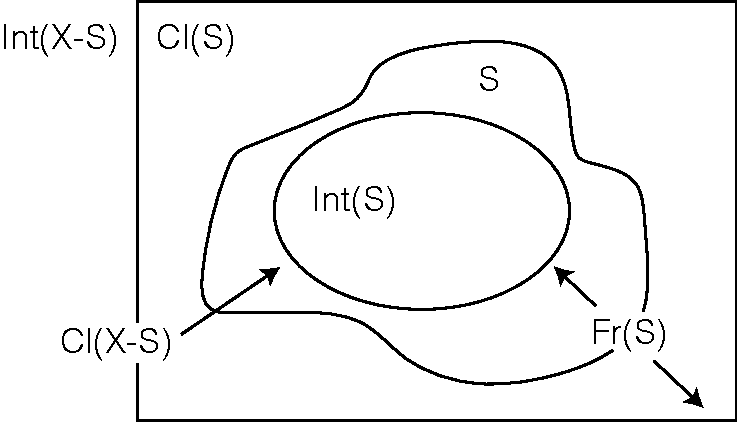
\includegraphics[width=0.4\textwidth ]{resources/chap_topo_spc/topospace1.pdf}  
	\caption{Illustration of the closure, interior and frontier of a set $S$.}
	\label{fig:topospace1}
\end{figure}

\begin{corollary}
	Let $X$ be a space and $S\subseteq X$. There're at most 14 distinct sets one can get from $X$ by applying the operations of closure and complement, namely:
	\begin{eqnarray}
		&&A,\ A^{\neg},\ A^{\neg-},\ A^{\neg-\neg},\ A^{\neg-\neg-},\ A^{\neg-\neg-\neg},\ A^{\neg-\neg-\neg-},\ A^{\neg -\neg-\neg-\neg},\nonumber \\
		&&A^-,\ A^{-\neg},\ A^{-\neg-},\ A^{-\neg-\neg},\ A^{-\neg-\neg-},\ A^{-\neg-\neg-\neg}
	\end{eqnarray}
\end{corollary}
\begin{proof}
	An example that gives the 14 distinct sets is:
	\begin{eqnarray}
		A&=&(-1,0)\cup(0,1)\cup(\mathbb Q\cap(1,2))\cup\{3\}\\
		A^{\neg}&=&(-\infty,-1]\cup\{0\}\cup([1,2]-\mathbb Q)\cup [2,3)\cup(3,\infty)\\
		A^{\neg-}&=&(-\infty,-1]\cup\{0\}\cup[1,\infty)\\
		A^{\neg-\neg}&=&(-1,0)\cup(0,1)\\
		A^{\neg-\neg-}&=&[-1,1]\\
		A^{\neg-\neg-\neg}&=&(-\infty,-1)\cup(1,\infty)\\
		A^{\neg-\neg-\neg-}&=&(-\infty,-1]\cup[1,\infty)\\
		A^{\neg -\neg-\neg-\neg}&=&(-1,1)\\
		A^{-}&=&[-1,2]\cup\{3\}\\
		A^{-\neg}&=&(-\infty,-1)\cup (2,3)\cup(3,\infty)\\
		A^{-\neg-}&=&(-\infty,-1]\cup [2,\infty)\\
		A^{-\neg-\neg}&=&(-1,2)\\
		A^{-\neg-\neg-}&=&[-1,2]\\
		A^{-\neg-\neg-\neg}&=&(-\infty,-1)\cup (2,\infty)
	\end{eqnarray}
	
	The preceding lemma tells us that there's no more.
\end{proof}

\begin{lemma}[Kuratowski]
	The operation $A\rightarrow A^-$ in a topological space $X$ has the following properties:
	\begin{enumerate}
		\item [K1] $A\subseteq A^-$,
		\item [K2] $A^{--}=A^-$,
		\item [K3] $(A\cup B)^-=A^-\cup B^-$,
		\item [K4] $\emptyset^-=\emptyset$,
	\end{enumerate}
	and furthermore
	\begin{enumerate}
		\item [K5] $A$ is closed in $X$ if $A=A^-$.
	\end{enumerate}
	
	If we have a set $X$ and a map $A\rightarrow A^-$ for each $A\subseteq X$ that satisfies K1-K4. Then $X$ becomes a topology space if the closed sets are defined by K5. The map $A\rightarrow A^-$ in $X$ coincides with the one we began with.
	\label{lem:Kurato}
\end{lemma}
\begin{proof}
	K3 $\rightarrow ((A\subseteq B)\rightarrow B^-=(A\cup(B-A))^-=A^-\cup(B-A)^-)\rightarrow((A\subseteq B)\rightarrow (A^-\subseteq B^-))$
\end{proof}

\begin{lemma}
	The operation $A\rightarrow A^\circ$ in a topological space $X$ has the following properties:
	\begin{enumerate}
		\item [I1] $A^\circ\subseteq A$,
		\item [I2] $A^{\circ\circ}=A^\circ$,
		\item [I3] $(A\cap B)^\circ=A^\circ\cap B^\circ$,
		\item [I4] $X^\circ=X$,
	\end{enumerate}
	and furthermore
	\begin{enumerate}
		\item [I5] $A$ is open in $X$ if $A=A^\circ$.
	\end{enumerate}
	
	If we have a set $X$ and a map $A\rightarrow A^\circ$ for each $A\subseteq X$ that satisfies I1-I4. Then $X$ becomes a topology space if the open sets are defined by I5. The map $A\rightarrow A^\circ$ in $X$ coincides with the one we began with.
\end{lemma}

\begin{definition}
	Let $S$ be a subset of $X$. $x$ is a {\bf limit point} of $S$ iff for each neighborhood $N$ of $x$, $(N-\{x\})\cap S\neq \emptyset$.
\end{definition}

\begin{lemma}
	Let $(X,\mathcal T)$ be a topological space, $x\in X$ and $S\subseteq X$. $S^-=S\cup\{$ all the limit points of $S\}$.
\end{lemma}

\begin{definition}
	Let $S$ be a closed subset of $X$, and $T\subseteq S$. $T$ is called {\bf dense} in $S$ if $T^-=S$.
\end{definition}

\section{Subspace}

\begin{definition}
	Let $(X,\mathcal T)$ be a topological space and $Y\subseteq X$. The topological space $(Y,\{S\cap Y|S\in \mathcal T\})$ is called {\bf a subspace} of $(X,\mathcal T)$.
\end{definition}

\begin{theorem}
	Let $Y$ be a subspace of a topological space $X$, then
	\begin{enumerate}
		\item $H\subseteq Y$ is open in $A$ iff $H=G\cap A$ where $G$ is open in $X$.
		\item $H\subseteq Y$ is closed in $A$ iff $H=G\cap A$ where $G$ is closed in $X$.
		\item Let $H\subseteq Y$. Then $Cl_Y(H)=Y\cap Cl_X(H),Int_Y(H)=Y\cap Int_X(H),Fr_Y(H)=Y\cap Fr_X(H)$.
		\item Let $x\subseteq Y$. If $\mathcal B_x$ is a neighborhood base(local base) at $x$ in $X$, then $\{B\cap Y|B\in\mathcal B_x\}$ is a neighborhood base(local base) at $x$ in $Y$.
		\item If $\mathcal B$ is a base(subbase) for $X$, then $\{B\cap Y|B\in\mathcal B\}$ is a base(subbase) for $Y$
	\end{enumerate}
\end{theorem}

\section{Metric Spaces}
\begin{definition}
	Let $X$ be a set and $\rho:X\times X\mapsto\mathbb R$ be a map. $\rho$ is called a {\bf pseudometric} on $X$ if for all $x,y\in X$:
	\begin{enumerate}
		\item $\rho(x,y)\geq 0$
		\item $\rho(x,x)= 0$
		\item $\rho(x,y)=\rho(y,x)$
		\item $\rho(x,y)+\rho(y,z)\geq\rho(x,z)$
	\end{enumerate}
	$\rho$ is called a {\bf metric} on $X$ if it's a pseudometric and $\rho(x,y)=0\Rightarrow x=y$.
\end{definition}
\begin{definition}
	We define the {\bf ball} in $X$ centered at $x$ as $B(x,r)=\{y\in  X|\rho(x,y)<r\}$.
\end{definition}

\begin{definition}
	Let $X$ be a set with a pseudometric $\rho$. $X$ is called a {\bf pseudometric space} if it has the topology with $\{B(x,r)| r>0\}$ as a local base at $x$.
\end{definition}

\begin{definition}
	A {\bf metric space} is a pseudometric space whose pseudometric is a metric.
\end{definition}

\begin{lemma}
	Let $X$ be a pseudometric space with pseudometric $\rho$, $\sim$ be the equivalence relation on $X$ defined by $x\sim y\leftrightarrow\rho(x,y)=0$. Let $X^*=X/\sim$ be the equivalence classes. We define a map $\rho^*:X^*\times X^*\mapsto\mathbb R$ as $\rho^*([x],[y])=\rho(x,y)$. $\rho^*$ is well-defined and is a metric on $X^*$.
	\label{lem:metric_equi}
\end{lemma}

\section{Examples}

\begin{example}
	We define the {\bf discrete topology} on a set $X$ as the family of all subsets of $X$.
\end{example}

\begin{example}
	We define the {\bf trivial topology} on a set $X$ as $\{\emptyset,X\}$.
\end{example}

\begin{example}
	Let $X$ be a infinite set, we define the {\bf cofinite topology} on $X$ by $\{S\in \mathcal T||X-S|<\aleph_0\vee S=\emptyset\}$.
\end{example}

\begin{example}
	We define the {\bf usual topology} on $\mathbb R^n$ as the metric topology with the metric $\rho(x,y)=\sqrt{\sum_i(x_i-y_i)^2}$.
\end{example}

\begin{example}
	Let $X$ be a linearly ordered set, we define the {\bf order topology} on $X$ to be the one with the subbase $\{(-\infty,a),(a,\infty)|a\in X\}$.
\end{example}

\begin{example}
	We define the {\bf radial plane} as the real plane with the topology such that a local neighborhood base at $x$ is $\mathcal N_x=\{S\subset \mathbb R^2|S$ contains an open line segment through $x$ in each direction$\}$. See Fig. \ref{fig:radial}.
\end{example}

\begin{figure}[htb!]
	\centering  
	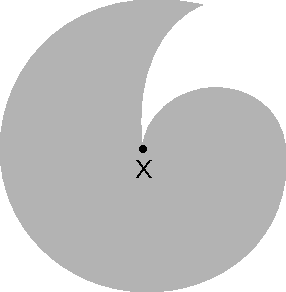
\includegraphics[width=0.2\textwidth ]{resources/chap_topo_spc/radial.pdf}  
	\caption{Example of neighborhood at $x$ of radial plane.}
	\label{fig:radial}
\end{figure}

\begin{example}
	We define the {\bf Sorgenfrey line} as the real line with the topology such that a local base at $x$ contains $[x,y)$ for all $y>x$.
\end{example}

\begin{example}
	We define the {\bf Moore plane} as the topology on the upper half plane $\{(x,y)\in \mathbb R^2|y\geq 0\}$, such that: At $(x,y)$ where $y>0$, a neighborhood base contains $2$-balls in the upper half plane centered at $(x,y)$. At $(x,0)$, a neighborhood base contains sets of the form $\{(x,0)\}\cap A$, where $A$ is a $2$-ball in the upper half plane tangent to the x-axis at $(x,0)$. See Fig. \ref{fig:moore}.
\end{example}

\begin{figure}[htb!]
	\centering  
	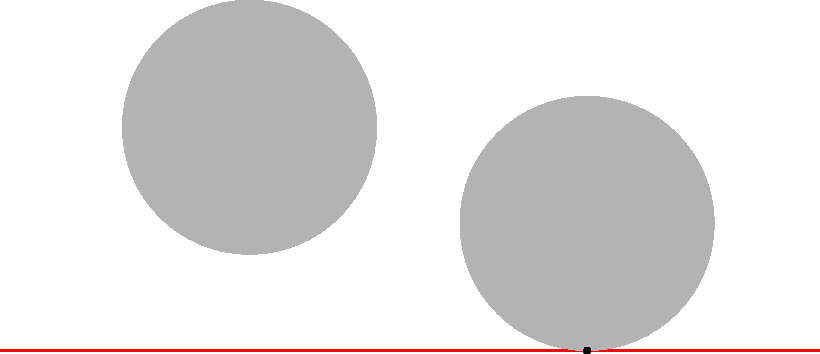
\includegraphics[width=0.5\textwidth ]{resources/chap_topo_spc/moore.pdf}  
	\caption{Example of neighborhoods of Moore plane.}
	\label{fig:moore}
\end{figure}

\chapter{Product and Quotient Spaces}
\section{Continuous Function}

\begin{definition}
	Let $X$ and $Y$be topological spaces and $f:X\mapsto Y$. $f$ is said to be {\bf continuous at} $x\in X$ if $\forall$ neighborhood $V$ of $f(x)\exists$ neighborhood $U$ of $x:f(U)\subseteq V$.
\end{definition}

\begin{definition}
	Let $X$ and $Y$be topological spaces and $f:X\mapsto Y$. $f$ is called a {\bf continuous function} if it satisfies the equivalent conditions:
	\begin{enumerate}
		\item $\forall x\in X:f$ is continuous at $x$.
		\item $H\subseteq Y$ is open $\Rightarrow f^{-1}(H)$ is open.
		\item $H\subseteq Y$ is closed $\Rightarrow f^{-1}(H)$ is closed.
		\item $\forall H\subseteq X: f(H^-)\subseteq f(H)^-$.
		\item $\forall H\subseteq Y: f^{-1}(H)^-\subseteq f^{-1}(H^-)$.
		\item $\forall H\subseteq X: f(H^\circ)\supseteq f(H)^\circ$.
		\item $\forall H\subseteq Y: f^{-1}(H)^\circ\supseteq f^{-1}(H^\circ)$.
	\end{enumerate}
\end{definition}

\begin{theorem}
	Let $f$ be a continuous function from $X$ to $Y$, and $U$ be a subspace of $X$. Then $f|_U$ is continuous.
\end{theorem}

\begin{definition}
	Let $X$ and $Y$be topological spaces and $f:X\mapsto Y$ be a bijective map. $f$ is called a {\bf homeomorphism} if both $f$ and $f^{-1}$ are continuous.
\end{definition}
\begin{theorem}
	Let $X$ and $Y$be topological spaces and $f:X\mapsto Y$ be a bijective map. The following are equivalent
	\begin{enumerate}
		\item $f$ is a homeomorphism.
		\item $H\subseteq Y$ is open $\Leftrightarrow f^{-1}(H)$ is open.
		\item $H\subseteq Y$ is closed $\Leftrightarrow f^{-1}(H)$ is closed.
		\item $\forall H\subseteq X: f(H^-)= f(H)^-$.
		\item $\forall H\subseteq Y: f^{-1}(H)^-= f^{-1}(H^-)$.
	\end{enumerate}
\end{theorem}

\begin{theorem}
	Let $f$ be a homeomorphism from $X$ to $Y$, and $U$ be a subspace of $X$. Then $f|_U$ is homeomorphism from $U$ to $f(U)$.
\end{theorem}

\begin{definition}
	Let $f$ be a continuous function from $X$ to $Y$. If $f$ is a homeomorphism from $X$ to $f(X)$, then $f$ is called an {\bf embedding}.
\end{definition}

\begin{definition}
	Let $f$ be a map from $X$ to $Y$. $f$ is called an {\bf open map} if it maps open subsets to open subsets. $f$ is called a {\bf closed map} if it maps closed subsets to closed subsets.
\end{definition}

\begin{example}
	For topological spaces $X$ and $Y$, let $C(X,Y)$ denote the collection of all continuous functions from $X$ to $Y$. Especially, we use $C(X)$ to denote $C(X,\mathbb R)$, and $C^*(X)$ to denote all bounded functions in $C(X)$. It's easy to see that $C(X)$ and $C^*(X)$ are algebras over $\mathbb R$. Moreover, $C^*(X)$ is a normed linear space with the norm $\|f\|=sup_{x\in X}|f(x)|$.
\end{example}
\section{Product Spaces and Weak Topologies}

\begin{definition}
	Let $X$ be a set and $X_\alpha$ be a topological spaces with $f_\alpha:X\mapsto X_\alpha$ for each $\alpha\in A$. The {\bf weak topology} induced on $X$ by $\{f_\alpha|\alpha\in A\}$ is the weakest topology on $X$ making each $f_\alpha$ continuous.
\end{definition}

\begin{theorem}
	Let $X$ be a set and $X_\alpha$ be a topological spaces with $f_\alpha:X\mapsto X_\alpha$ for each $\alpha\in A$. The weak topology induced on $X$ by $\{f_\alpha|\alpha\in A\}$ is the one with the subbase $\{f^{-1}_\alpha(U_\alpha)|\alpha\in A, U_\alpha$ open in $X_\alpha\}$
\end{theorem}

\begin{theorem}
	Let $X_\alpha$ be topological spaces. Let $X$ be a set with weak topology induced by $f_\alpha:X\mapsto X_\alpha$ for each $\alpha\in A$. Let $Y$ be a topological space. A map $f:Y\mapsto X$ is continuous iff $f_\alpha\circ f$ is continuous for each $\alpha \in A$.
\end{theorem}

\begin{definition}
	Let $X_\alpha$ be a family of topological spaces where $\alpha\in A$, and $\prod_{\alpha\in A}X_\alpha$ be their Cartesian product. We define $\pi_\alpha: \prod_{\alpha\in A}X_\alpha\mapsto X_\alpha$ as $\pi_\alpha(x)=x_\alpha$. Then the weakest topology induced on $\prod_{\alpha\in A}X_\alpha$ by  $\{\pi_\alpha|\alpha\in A\}$ is called the {\bf product topology}. With this topology, $\prod_{\alpha\in A}X_\alpha$ is called the {\bf product space}.
\end{definition}
\begin{theorem}
	Let $X_\alpha$ be a family of spaces where $\alpha\in A$, then their product space is the direct product of $X_\alpha$ in the category {\bf Top}.
\end{theorem}

\begin{theorem}
	Let $X_\alpha$ be a family of spaces where $\alpha\in A$, and $\prod_{\alpha\in A}X_\alpha$ be their product space. Then $\pi_\alpha: \prod_{\alpha\in A}X_\alpha\mapsto X_\alpha$ is an open map for each $\alpha \in A$.
\end{theorem}

\begin{theorem}
	A map $f:X\mapsto\prod_\alpha X_\alpha$ is continuous iff $\pi_\alpha\circ f$ is continuous for each $\alpha\in A$.
\end{theorem}

\begin{definition}
	Let $X$ be a space and $X_\alpha$ be spaces, with $f_\alpha:X\mapsto X_\alpha$ for each $\alpha\in A$. The {\bf evaluation map} $e:X\mapsto \prod_\alpha X_\alpha$ is defined by $e(x)=\bar x$, where $\bar x_\alpha=f_\alpha(x)$.
\end{definition}

\begin{theorem}
	Let $X$ be a space and $X_\alpha$ be spaces, with $f_\alpha:X\mapsto X_\alpha$ for each $\alpha\in A$. Then the evaluation map $e:X\mapsto \prod_\alpha X_\alpha$
	\begin{enumerate}
		\item is continuous iff $f_\alpha$ is continuous for each $\alpha\in A$.
		\item is injective iff $\forall x\neq y\in X\exists \alpha\in A:f_\alpha(x)\neq f_\alpha(y)$.
		\item is an embedding iff it's injective and $X$ has the weak topology induced by $f_\alpha$.
	\end{enumerate}
	\label{thm:weak_embed}
\end{theorem}
\begin{proof}
	1: $f_\alpha=\pi_\alpha\circ e$
	
	3: If $e$ is injective and $X$ has the weak topology induced by $f_\alpha$, it's easy to see that $e$ is continuous. We only need to prove that $e$ is open (from $X$ to $e(X)$), which only needs to be tested on a subbase of $X$: $\{f^{-1}_\alpha(U_\alpha)|\alpha\in A, U_\alpha$ open in $X_\alpha\}$. However $e(f^{-1}_\alpha(U_\alpha))=e(X)\cap \pi_\alpha^{-1}(U_\alpha)$, which is open in $e(X)$.
	
	If $e$ is an embedding, then $e$ is injective. It's easy to see that $X$ has the weak topology induced by $e$. Since $\prod_\alpha X_\alpha$ has the weak topology induced by $\{\pi_\alpha\}$. $X$ has the weak topology induced by $\{f_\alpha\}=\{\pi_\alpha\circ e\}$.
\end{proof}

\begin{theorem}
	Let $X$ be a pseudometric space with pseudometric $\rho:X\times X\mapsto \mathcal R$. $\rho$ is a continuous function.
\end{theorem}
\section{Coproduct Spaces and Strong Topologies}

\begin{definition}
	Let $X$ be a set and $X_\alpha$ be a topological spaces with $f_\alpha:X_\alpha \mapsto X$ for each $\alpha\in A$. The {\bf strong topology} induced on $X$ by $\{f_\alpha|\alpha\in A\}$ is the strongest topology on $X$ making each $f_\alpha$ continuous.
\end{definition}

\begin{theorem}
	Let $X$ be a set and $X_\alpha$ be a topological spaces with $f_\alpha:X_\alpha \mapsto X$ for each $\alpha\in A$. The strong topology induced on $X$ by $\{f_\alpha|\alpha\in A\}$ is the one with the open sets $\{S\subseteq X|\forall \alpha\in A:f^{-1}_\alpha(S)$ is open in $X_\alpha\}$
\end{theorem}

\begin{theorem}
	Let $X_\alpha$ be topological spaces. Let $X$ be a set with strong topology induced by $f_\alpha:X_\alpha\mapsto X$ for each $\alpha\in A$. Let $Y$ be a topological space. A map $f:X\mapsto Y$ is continuous iff $f\circ f_\alpha$ is continuous for each $\alpha \in A$.
\end{theorem}


\begin{corollary}
	Let $f$ be a function from $X$ to $Y$, and $U_\alpha$ be a family of open subspaces of $X$ that covers $X$. If $\forall \alpha:f|_{U_\alpha}$ is continuous, then $f$ is continuous.
\end{corollary}
\begin{proof}
	$X$ has the strong topology induced by the inclusion map $\{U_\alpha\mapsto X\}$.
\end{proof}

\begin{definition}
	Let $X_\alpha$ be a family of topological spaces where $\alpha\in A$, and $\coprod_{\alpha\in A}X_\alpha$ be their disjoint union. We define $\iota_\alpha:X_\alpha\mapsto \coprod_{\alpha\in A}X_\alpha $ as $\iota_\alpha(x_\alpha)=x_\alpha$. Then the strong topology induced on $\coprod_{\alpha\in A}X_\alpha$ by  $\{\iota_\alpha|\alpha\in A\}$ is called the {\bf coproduct topology}. With this topology, $\coprod_{\alpha\in A}X_\alpha$ is called the {\bf coproduct space}.
\end{definition}

\begin{theorem}
	Let $X_\alpha$ be a family of topological spaces where $\alpha\in A$, then their coproduct space is the direct sum of $X_\alpha$ in the category {\bf Top}.
\end{theorem}

\begin{theorem}
	Let $X_\alpha$ be a family of topological spaces where $\alpha\in A$, and $\coprod_{\alpha\in A}X_\alpha$ be their coproduct space. Then $\iota_\alpha: X_\alpha\mapsto\coprod_{\alpha\in A}X_\alpha$ is an open map for each $\alpha \in A$.
\end{theorem}
\section{Quotient map and Quotient Spaces}

\begin{definition}
	Let $f:X \mapsto Y$ be a surjective map from a topological space $X$ to a set $Y$. The {\bf quotient topology} on $Y$ induced by $f$ is the coproduct topology.
\end{definition}

\begin{lemma}
	Let $X$ be a set and $X_\alpha$ be a topological spaces with $f_\alpha:X_\alpha \mapsto X$ for each $\alpha\in A$. We define a map $f:\coprod_{\alpha\in A}X_\alpha\mapsto X$ by $f(x_\alpha)=f_\alpha(x_\alpha)$. Then $X$ has the strong topology induced by $(f_\alpha)$ iff it has the quotient topology induced by $f$.
\end{lemma}

\begin{definition}
	Let $X$ and $Y$ be topological spaces with an surjective map $f:X \mapsto Y$. $f$ is called the {\bf quotient map} if the topology on $Y$ is the quotient topology induced by $f$.
\end{definition}

\begin{definition}
	Let $X$ be a topological space and $\sim$ be an equivalence relation on $X$. The {\bf quotient space} of $X$ induced by $\sim$ is $X/\sim$ with the quotient topology induce by the canonical map $X\mapsto X/\sim$. If an equivalence relation on $X$ is $a\sim b\leftrightarrow a,b\in A\subseteq X$, then the quotient space may also be written as $X/A$.
\end{definition}

\begin{lemma}
	Let $X$ and $Y$ be topological spaces with a map $f:X \mapsto Y$. We define an equivalence relation on $X$ by $x\sim y\leftrightarrow f(x)=f(y)$. Then $f(X)\simeq X/\sim$. 
\end{lemma}

\begin{definition}
	We define an $n$-dimensional {\bf disk} to be $D^n=\{x\in \mathbb R^n||x|\leq 1\}$. We define $\partial D^n=\{x\in \mathbb R^n||x|= 1\}$
\end{definition}

\begin{lemma}
	$S^n\simeq D^n/\partial D^n$
\end{lemma}
\begin{proof}
	Consider the map $f:D^n\mapsto S^n$
	\begin{equation}
		f(x)=(1-2|x|,2\sqrt{\frac{1-|x|}{|x|}}x_0,\cdots,,2\sqrt{\frac{1-|x|}{|x|}}x_{n-1})
	\end{equation}
\end{proof}

\begin{theorem}
	A surjective continuous map is a quotient map if it's open or closed.
\end{theorem}
\begin{proof}
	If $f:X\mapsto Y$ is a surjective continuous closed map. Let $T$ be a set in $Y$ such that $f^{-1}(T)$ is open. Then $Y-T=f(X-f^{-1}(T))$ is closed. So $T$ is open.
\end{proof}

\begin{example}
	How to stick two spaces together? Let $A$ and $B$ be two topological spaces, we consider their coproduct space $A\sqcup B$. We can define some equivalence relation on $A\sqcup B$, and the quotient space $A\sqcup B/\sim$ would be the $A$ and $B$ stuck together.
\end{example}

\chapter{Convergence}

\section{Moore-Smith Convergence}

\begin{definition}
	A {\bf directed set} is a set $S$ with a pre-order $\leq$ such that any two elements are bounded. We say that $S$ is {\bf directed by} $\leq$.
\end{definition}

\begin{definition}
	Let $\Lambda$ be a directed set. A {\bf net} $(x_\lambda)$ is a map from $\Lambda$ to $X$.
\end{definition}

\begin{definition}
	Let $(x_\lambda)$ be a net from $\Lambda$ to $X$, and $S\subseteq X$. $(x_\lambda)$ is said to be {\bf eventually in} $S$ if $\exists \lambda_0:\lambda>\lambda_0\rightarrow x_\lambda\in S$. $(x_\lambda)$ is said to be {\bf frequently in} $S$ if $\forall \lambda_0\exists\lambda>\lambda_0: x_\lambda\in S$. It's easy to see that ``not eventually in $S$" is equivalent to ``frequently in $X-S$", and ``not frequently in $S$" is equivalent to ``eventually in $X-S$"
\end{definition}

\begin{definition}
	Let $(x_\lambda)$ be a net from $\Lambda$ to $X$. $(x_\lambda)$ is said to {\bf converges to} $x_0$ (written as $x_\lambda\rightarrow x_0$) if it's eventually in each neighborhood of $x_0$.
\end{definition}

\begin{definition}
	Let $(x_\lambda)$ be a net from $\Lambda$ to $X$. $x_0$ is said to be a {\bf cluster point} of $(x_\lambda)$ if the net is frequently in each neighborhood of $x_0$.
\end{definition}

\begin{example}
	Let $X$ be a topological space and $x\in X$. Let $\Lambda$ be a neighborhood base at $x$. Then $\Lambda$ with the order relation $U_1\leq U_2$ iff $U_1\supseteq U_2$ forms a directed set. If we pick a $x_U\in U$ for each $U\in\Lambda$ (using AC), we result in a net $(x_U)$ that converges to $x$.
\end{example}

\begin{definition}
	Let $(x_\lambda)$ be a net from $\Lambda$ to $X$. A net $(x'_\mu)$ from $M$ to $X$ is a {\bf subnet} of $(x_\lambda)$ if there's an increasing cofinal function $\phi:M\mapsto\Lambda$ such that $x'_\mu=x_{\phi(\mu)}$.
\end{definition}

\begin{theorem}
	Let $(x_\lambda)$ be a net from $\Lambda$ to $X$ frequently in $E\subseteq X$. Then there is a subnet of $(x_\lambda)$ eventually in $E\subseteq X$.
\end{theorem}

\begin{theorem}
	Let $(x_\lambda)$ be a net from $\Lambda$ to $X$ eventually in $E\subseteq X$. Then all of its subnets are eventually in $E\subseteq X$.
\end{theorem}

\begin{theorem}
	If a net from $\Lambda$ to $X$ converges to $x$, then all of its subnets converge to $x$.
\end{theorem}

\begin{theorem}
	A net from $\Lambda$ to $X$ has $x$ as a cluster point iff it has a subnet that converges to $x$.
	\label{thm:subnet}
\end{theorem}
\begin{proof}
	Let $(x_\lambda)$ be a net $\Lambda\mapsto X$. We define $\Lambda'=\{(\lambda,U)\in\Lambda\times P(X)|x_\lambda\in U $ is a neighborhood of $x\}$. $\Lambda'$ is directed by the pre-order: $(\lambda,U)\leq(\lambda',U')$ iff $\lambda\leq\lambda'$ and $U\supseteq U'$. We define $\theta:\Lambda'\mapsto \Lambda$ as $\theta(\lambda,U)=\lambda$. Then $(x_{\theta(\lambda,U)})$ is a subnet that converges to $x$.
\end{proof}

\begin{theorem}
	Let $X$ be a topological space and $E\subseteq X$. Then $x\in E^-$ iff there is a net from $\Lambda$ to $E$ that converges to $x$.
\end{theorem}

This theorem together with Lem. \ref{lem:Kurato} tell us that the topology of a space is determined by the convergence of nets in it.

\begin{theorem}
	Let $f:X\mapsto Y$. Then $f$ is continuous at $x_0\in X$ iff for each net $x_\lambda\rightarrow x_0$ we have $f(x_\lambda)\rightarrow f(x_0)$.
\end{theorem}
\begin{proof}
	$f$ is continuous at $x_0\in X$ 
	
	iff $(\forall $ open $U\ni f(x_0))x_0\in f^{-1}(U)^\circ$ 
	
	iff $(\forall $ open $U\ni f(x_0))$ and $\forall x_\lambda\rightarrow x_0$, $(x_\lambda)$ is eventually in $f^{-1}(U)$.
	
	iff $(\forall $ open $U\ni f(x_0))$ and $\forall x_\lambda\rightarrow x_0$, $f(x_\lambda)$ is eventually in $U$.
	
	iff $\forall x_\lambda\rightarrow x_0$,$f(x_\lambda)\rightarrow f(x_0)$.
\end{proof}

\begin{definition}
	Let $(x_\lambda)$ be a net from $\Lambda$ to $X$. $(x_\lambda)$ is said to be an {\bf ultranet} iff for each $E\subseteq X$, $(x_\lambda)$ is either eventually in $E$ or eventually in $X-E$.
\end{definition}

\begin{theorem}
	Every subnet of an ultranet is an ultranet.
\end{theorem}

\begin{theorem}
	If an ultranet has $x$ as a cluster point, then it converges to $x$.
\end{theorem}

\section{Filters}

\begin{definition}
	A {\bf filter} $\mathcal F$ on a set $X$ is a nonempty collection of nonempty subsets of $S$ such that 
	\begin{enumerate}
		\item if $F_1,F_2\in \mathcal F$, then $F_1\cap F_2\in \mathcal F$
		\item if $F_1\in \mathcal F$ and $F_1\subseteq F_2$, then $F_2\in \mathcal F$
	\end{enumerate}
\end{definition}

\begin{definition}
	Let $\mathcal F$ be a filter on $X$. A subcollection $\mathcal C$ of $\mathcal F$ is called a {\bf filter base} iff $(\forall F\in\mathcal F)(\exists C\in \mathcal C) C\subseteq F$.
\end{definition}

\begin{lemma}
	Let $\mathcal C$ be a filter base of the filter $\mathcal F$. Then $(\forall C_1,C_2\in \mathcal C)(\exists C\in \mathcal C)C\subseteq C_1\cap C_2$.
\end{lemma}

\begin{lemma}
	Let $\mathcal C$ be a collection of nonempty subsets of $X$. $\mathcal C$ is a filter base for some filter iff $(\forall C_1,C_2\in \mathcal C)(\exists C\in \mathcal C)C\subseteq C_1\cap C_2$. If $\mathcal C$ satisfies this condition, then its a filter base of the filter $\mathcal F=\{F\subseteq X|(\exists C\in \mathcal C)C\subseteq F\}$. We also call $\mathcal F$ the filter generated by $\mathcal C$.
\end{lemma}


\begin{definition}
	Let $\mathcal F$ be a filter on $X$. A subcollection $\mathcal C$ of $\mathcal F$ is called a {\bf filter subbase} iff all finite intersections of $\mathcal C$ is a filter base of $\mathcal F$.
\end{definition}

\begin{lemma}
	Let $\mathcal C$ be a collection of nonempty subsets of $X$. $\mathcal C$ is a filter subbase for some filter iff each finite intersection of $\mathcal C$ is nonempty.
\end{lemma}

\begin{definition}
	Let $\mathcal F_1$ and $\mathcal F_2$ be two filters on $X$. We say $\mathcal F_1$ is {\bf finer} that $\mathcal F_2$ iff $\mathcal F_1\supseteq\mathcal F_2$
\end{definition}

\begin{definition}
	Let $\mathcal F$ be a filter on $X$. We say $\mathcal F$ is {\bf fixed} iff $\bigcap F\neq\emptyset$. We say $\mathcal F$ is {\bf free} iff $\bigcap F=\emptyset$.
\end{definition}

\begin{example}
	Let $X$ be a topological space and $x\in X$. The neighborhood $\mathcal U_x$ of $x$ is a filter called the {\bf neighborhood filter}.
\end{example}

\begin{example}
	Let $X$ be a set and $S\subseteq X$. Then $\{T\subseteq X|S\subseteq T\}$ is a filter called the {\bf principle filter} at $S$.
\end{example}

\begin{example}
	Let $X$ be a set. The {\bf Fr\'echet filter} on $X$ is defined as the collection of cofinite subsets in $X$. It's easy to see that the Fr\'echet filter is free.
\end{example}

\begin{definition}
	Let $\mathcal F$ be a filter on a topological space $X$. $\mathcal F$ is said to {\bf converge to} $x$ (written as $\mathcal F\rightarrow x$) iff $\mathcal F$ is finer than the neighborhood filter $\mathcal U_x$ at $x$.
\end{definition}

\begin{definition}
	Let $\mathcal F$ be a filter on a topological space $X$. $\mathcal F$ is said to have $x$ as a {\bf cluster point} iff $\forall F\in \mathcal F: x\in F^-$.
\end{definition}

\begin{theorem}
	Let $\mathcal F$ be a filter on $X$. $\mathcal F$ has $x$ as a cluster point iff there's a filter finer than $\mathcal F$ that converges to $x$.
\end{theorem}

\begin{theorem}
	Let $X$ be a topological space and $E\subseteq X$. Then $x\in E^-$ iff there is a filter that contains $E$ and converges to $x$.
\end{theorem}

This theorem together with Lem. \ref{lem:Kurato} tell us that the topology of a space is determined by the convergence of filters in it.

\begin{definition}
	Let $\mathcal F$ be a filter on $X$, and $f:X\mapsto Y$. We define $f(\mathcal F)$ as a filter in $Y$ with filter base $\{f(F)|F\in\mathcal F\}$.
\end{definition}

\begin{theorem}
	Let $f:X\mapsto Y$. Then $f$ is continuous at $x_0\in X$ iff for each filter $\mathcal F\rightarrow x_0$ we have $f(\mathcal F)\rightarrow f(x_0)$.
\end{theorem}
\begin{proof}
	$f$ is continuous at $x_0\in X$ 
	
	iff $(\forall $ open $U\ni f(x_0))x_0\in f^{-1}(U)^\circ$ 
	
	iff $(\forall $ open $U\ni f(x_0)) f^{-1}(U)\in\mathcal U_{x_0}$ 
	
	iff $(\forall $ open $U\ni f(x_0))U\in f(\mathcal U_{x_0})$ 
	
	iff $ f(\mathcal U_{x_0})\rightarrow f(x_0)$ 
	
	iff $\forall\mathcal F\rightarrow x_0$ we have $f(\mathcal F)\rightarrow f(x_0)$.
\end{proof}

\begin{definition}
	Let $\mathcal F$ be a filter on $X$. $\mathcal F$ is said to be an ultrafilter iff there is no filter strictly finer than $\mathcal F$.
\end{definition}

\begin{theorem}
	Let $\mathcal F$ be a filter on $X$. $\mathcal F$ is an ultrafilter iff for each $E\subseteq X$, $E\in \mathcal F$ or $X-E\in \mathcal F$.
\end{theorem}

\begin{theorem}
	Every filter is contained in some ultrafilter.
\end{theorem}
\begin{proof}
	Let $\mathcal F$ be a filter. Let $FT$ be the set of all filters of $X$ that contains $\mathcal F$. $FT$ is directed by $\subseteq$. For each chain $C$ in $FT$, $\bigcup C$ is a upper bound of $C$. So by Zorn's lemma, there's a maximal element in $FT$, which is an ultrafilter that contains $\mathcal F$.
\end{proof}

\begin{theorem}
	If an ultrafilter has $x$ as a cluster point, then it converges to $x$.
\end{theorem}

\begin{theorem}
	A fixed untrafilter is a principle filter at some one-point set.
\end{theorem}

\section{Correspondence between Nets and Filters}

\begin{definition}
	Let $(x_\lambda)$ be a net on $X$. We define {\bf the filter generated by} $(x_\lambda)$ as the family of sets that $(x_\lambda)$ is eventually in. It has a filter base $\{\{x_\gamma|\gamma>\lambda\}\lambda\in\Lambda\}$.
\end{definition}

\begin{definition}
	Let $\mathcal F$ be a filter on $X$, and let $\Lambda=\{(x,F)|x\in F\in\mathcal F\}$. $\Lambda$ is directed by the relation $(x_1,F_1)\leq (x_2,F_2)$ iff $F_1\supseteq F_2$. We define {\bf the net based on} $\mathcal F$ by the map $f:\Lambda\mapsto X$ where $f(x,F)=x$.
\end{definition}

Note that this direct set is not partially ordered by $\leq$ (if $X$ contains at least 2 points).

\begin{theorem}
	Let $(x_\lambda)$ be a net on $X$. Let $(x_\lambda)$ generates a filter $\mathcal F$. Then
	\begin{enumerate}
		\item $(x_\lambda)$ is eventually in a set $S\subseteq X$ iff $S\in\mathcal F$.
		\item $(x_\lambda)$ is frequently in a set $S\subseteq X$ iff $X-S\not\in\mathcal F$, iff $\forall F\in \mathcal F:S\cap F\neq\emptyset$.
		\item $(x_\lambda)$ converges to $x\in X$ iff $\mathcal F$ converges to $x$.
		\item $(x_\lambda)$ has $x\in X$ as a cluster point iff $\mathcal F$ has $x$ as a cluster point.
		\item $(x_\lambda)$ is an ultranet iff $\mathcal F$ is an ultrafilter.
		\item A subnet of $(x_\lambda)$ generate a filter finer than $\mathcal F$.
		\item Let $\mathcal F'$ be a filter finer than $\mathcal F$. Then $\forall F\in \mathcal F':(x_\lambda)$ is frequently in $F$.
	\end{enumerate}
\end{theorem}

\begin{theorem}
	Let $\mathcal F$ be a filter on $X$, and $(x_\lambda)$ be a net based on $\mathcal F$. Then $(x_\lambda)$ generates $\mathcal F$.
\end{theorem}

\begin{lemma}
	Let $(x_\lambda)$ be a net on $X$ and $\mathcal F$ be a filter on $X$ such that $\forall F\in \mathcal F:(x_\lambda)$ is frequently in $F$. Then $(x_\lambda)$ has a subnet $(x'_{\lambda'})$ such that $\forall F\in \mathcal F:(x'_{\lambda'})$ is eventually in $F$.
\end{lemma}
We can give a proof by a slight generalization on the proof of the Thm. \ref{thm:subnet}, which treats the special case that $\mathcal F=\mathcal U_x$.
\begin{proof}
	We define $\Lambda'=\{(\lambda,F)\in\Lambda\times \mathcal F|x_\lambda\in F\}$. $\Lambda'$ is directed by the partial order: $(\lambda,F)\leq(\lambda',F')$ iff $\lambda\leq\lambda'$ and $F\supseteq F'$. We define $\theta:\Lambda'\mapsto \Lambda$ as $\theta(\lambda,F)=\lambda$. Then $(x_{\theta(\lambda,F)})$ is a subnet that is eventually in each $F\in \mathcal F$.
\end{proof}

\begin{corollary}
	Let $(x_\lambda)$ be a net on $X$ that generates a filter $\mathcal F$, and $\mathcal F'$ be a filter finer than $\mathcal F$. Then $(x_\lambda)$ has a subnet that generates a filter finer than $\mathcal F'$.
\end{corollary}

\begin{corollary}[Kelley]
	Every net has a subnet that is an ultranet.
\end{corollary}
\begin{proof}
	Let $(x_\lambda)$ be the net, which generates a filter $\mathcal F$. Let $\mathcal F'$ be an ultrafilter finer than $\mathcal F$. Then $(x_\lambda)$ has a subnet $(x'_{\lambda'})$ that generates a filter finer than $\mathcal F'$. However, since $\mathcal F'$ is an ultrafilter, $(x'_{\lambda'})$ generates $\mathcal F'$. So $(x'_{\lambda'})$ is an ultranet.
\end{proof}
\section{Sequential Space}

We have shown that the topology of a space is determined by the convergence of nets/filters in it. We may define a space whose topology space is determined by the convergence of sequences in it.

\begin{definition}
	Let $X$ be a topological space. $X$ is a {\bf sequential space} iff for each $E\subseteq X$, $E$ is closed iff for each converging sequence in $E$ converges to a point in $E$.
\end{definition}

\begin{definition}
	Let $X$ be a topological space. $X$ is a {\bf Fr\'echet-Urysohn space} iff for each $E\subseteq X$, $x\in E^-$ iff there is a sequence in $E$ that converges to $x$.
\end{definition}
\begin{theorem}
	A space is a Fr\'echet-Urysohn space if and only if every subspace is a sequential space.
\end{theorem}
\begin{proof}
	Let $X$ be a Fr\'echet-Urysohn space, and $S$ be a subspace. For each subset $E$ of $S$. 1. If $E$ is closed, let $E=E'\cap S$ where $E'$ is closed in $X$. Let $(x_n)$ be a sequence in $E$ that converges to $x$ in $S$. It's easy to see that $(x_n)$ converges to $x$ in $X$. So $x\in E'^-=E'$ in $X$. So $x\in E$. 2. If for each sequence in $E$ that converges to $x$ we have $x\in E$. We define $E_1$ to be $E^-$ in $S$ and $E_2$ to be $E^-$ in $X$. Clearly $E_1=E_2\cap S$. For each $y\in E_1\subseteq E_2$. Let $(x_n)$ be a sequence in $E$ that converges to $y$. So $E=E_1$ is closed in $S$.
	
	Let $X$ be a space such that every subspace is a sequential space. For each $E\subseteq X$. Consider the subspace $S=E\cup\{x\}$. Since $S$ is a sequential space, $x\in E^-\leftrightarrow E$ is not closed in $S\leftrightarrow$ there's a sequence in $E$ that converges to $x$.
\end{proof}

\begin{corollary}
	The subspace of a Fr\'echet-Urysohn space is a Fr\'echet-Urysohn space.
\end{corollary}

\begin{theorem}
	Let $X$ be a sequential space, and $f:X\mapsto Y$. Then $f$ is continuous at $x_0\in X$ iff for each sequence $(x_n)\rightarrow x_0$ we have $f(x_n)\rightarrow f(x_0)$.
\end{theorem}
\begin{proof}
	$f$ is continuous at $x_0\in X$ 
	
	iff $(\forall $ open $U\ni f(x_0))x_0\in f^{-1}(U)^\circ$ 
	
	iff $(\forall $ open $U\ni f(x_0))$ and $\forall x_n\rightarrow x_0$, $(x_n)$ is eventually in $f^{-1}(U)$.
	
	iff $(\forall $ open $U\ni f(x_0))$ and $\forall x_n\rightarrow x_0$, $f(x_n)$ is eventually in $U$.
	
	iff $\forall x_n\rightarrow x_0$,$f(x_n)\rightarrow f(x_0)$.
\end{proof}

\chapter{Separation and Countability}
In the first part of this chapter we propose some conditions of separation, that describe how separate two points or two closed sets are in a topological space. In the second part we propose some conditions of countability, that describe the countability of the basis of a topological space. The stricter condition a topological space satisfies, the better properties it will enjoy.
\section{$T_0$, $T_1$ and Hausdorff($T_2$) Spaces}
	\begin{definition}
		A {\bf $T_0$ space}, as shown in Fig.\ref{fig:T0}, is a topological space such that for each two different points $x$ and $y$, there is an open set that contains one and not the other.
	\end{definition}
	
	\begin{definition}
		A {\bf $T_1$ space}, as shown in Fig.\ref{fig:T1}, is a topological space such that for each two different points $x$ and $y$, each has a neighborhood that doesn't contain the other.
	\end{definition}
	
	\begin{definition}
		A topological space is a $T_1$ space iff each one point set is closed.
	\end{definition}
	
	\begin{definition}
		A topological space $X$ is a $T_1$ space iff for each $x\in X$, the union of all neighborhoods at $x$ is $\{x\}$.
	\end{definition}
	
	\begin{theorem}
		The closed image of a $T_1$ space is $T_1$.
	\end{theorem}
	
	\begin{definition}
		A {\bf $T_2$ space}, also called a {\bf Hausdorff space}, as shown in Fig.\ref{fig:T2}, is a topological space such that for each two different points $x$ and $y$, there are two disjoint open sets $S\ni x$ and $T\ni y$.
	\end{definition}
	
	\begin{theorem}
		A topological space is a Hausdorff space iff each net or filter only converges to at most one point.
	\end{theorem}
	
	\begin{proof}
		Let $X$ be a topological space that is not a $T_2$ space. Let $x,y\in X$ be two different points such that $\forall S\in \mathcal U_x,T\in \mathcal U_y:S\cap T\neq\emptyset$. (Remember that $\mathcal U_x$ is the neighborhood filter at $x$.) Let $\mathcal F=\{S\cap T|S\in \mathcal U_x,T\in \mathcal U_y\}$. It's easy to see that $\mathcal F$ is a filter that contains $\mathcal U_x$ and $\mathcal U_y$. So $\mathcal F$ converges to both $x$ and $y$.
	\end{proof}
	
	\begin{figure}[htb!]
		\centering  
		\begin{minipage}[t]{0.3\textwidth}  
		\centering  
		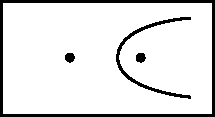
\includegraphics[width=150pt]{resources/chap_sep_count/T0.pdf}  
		\caption{$T_0$ space}
		\label{fig:T0}
		\end{minipage}  
		\begin{minipage}[t]{0.3\textwidth}  
		\centering  
		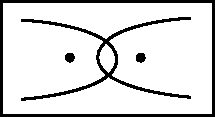
\includegraphics[width=150pt]{resources/chap_sep_count/T1.pdf}  
		\caption{$T_1$ space}  
		\label{fig:T1}
		\end{minipage}  
		\begin{minipage}[t]{0.3\textwidth}  
		\centering  
		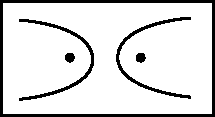
\includegraphics[width=150pt]{resources/chap_sep_count/T2.pdf}  
		\caption{$T_2$ space}  
		\label{fig:T2}
		\end{minipage}  
	\end{figure}
	
	\begin{definition}
		A {\bf Urysohn space}, also called a {\bf $T_{2\frac 12}$ space}, is a topological space such that for each two different points $x$ and $y$, there are two disjoint open sets $S\ni x$ and $T\ni y$ such that $S^-\cap T^-=\emptyset$.
	\end{definition}
	\begin{theorem}
		A Urysohn space is a $T_2$ space. A $T_2$ space is a $T_1$ space. A $T_1$ space is a $T_0$ space.
	\end{theorem}
	
	\begin{theorem}
		The subspace of a $T_0/T_1/T_2/$Urysohn space is $T_0/T_1/T_2/$Urysohn.
	\end{theorem}
	\begin{theorem}
		The product space is a $T_0/T_1/T_2/$Urysohn space iff each factor space is $T_0/T_1/T_2/$ Urysohn.
	\end{theorem}
	\begin{lemma}
		Let $X$ be a Hausdorff space, then the diagonal $\Delta(X)=\{(x,x)|x\in X\}$ is closed in $X\times X$. 
	\end{lemma}
	\begin{theorem}
		Let $Y$ be a Hausdorff space, and $f:X\mapsto Y$ and $f':X\mapsto Y$ be two continuous maps from $X$ to $Y$ that coincide on a dense subset of $X$. Then $f=f'$.
		\label{thm:Haus_dense}
	\end{theorem}
	\begin{proof}
		We define a continuous map $g: X\mapsto Y\times Y$ by $g(x)=(f(x),f'(x))$. $g^{-1}(\Delta(Y))$ is dense and closed in $X$. So $g^{-1}(\Delta(Y))=X$.
	\end{proof}
\section{Regular Spaces}
	\begin{definition}
		A space $X$ is a {\bf regular space}, as shown in Fig.\ref{fig:regular}, iff for each closed set $A\subseteq X$ and each $b\not \in A$, there are two disjoint open sets $S\supseteq A$ and $T\ni b$. A space $X$ is a {\bf $T_3$ space} iff its $T_1$ and regular.
	\end{definition}
	\begin{figure}[htb!]  
		\centering  
		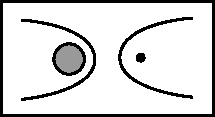
\includegraphics[width=150pt]{resources/chap_sep_count/regular.pdf}  
		\caption{Regular space}
		\label{fig:regular}
	\end{figure}
	\begin{theorem}
		A space $X$ is a regular space iff for each open set $A\subseteq X$ and each $x \in A$, there exists an open set $B\ni x$ such that $B^-\subseteq A$.
	\end{theorem}
	
	This means that regularity is a local property.
	
	\begin{theorem}
		A $T_0$ regular space is $T_3$.
	\end{theorem}
	
	\begin{definition}
		A space $X$ is a {\bf completely regular space} iff for each closed set $A\subseteq X$ and each $x\not \in A$, there exists a continuous function $f:X\mapsto I$ such that $f(x)=0$ and $f(A)=1$. A space $X$ is a {\bf Tychonoff space}, also called a $T_{3\frac 12}$ space, iff its $T_1$ and completely
		 regular.
	\end{definition}
	
	\begin{theorem}
		A Tychonoff space is a $T_3$ space. A $T_3$ space is a Urysohn space. A completely regular space is a regular space.
	\end{theorem}
	
	\begin{theorem}
		The subspace of a regular$/T_3/$completely regular$/$Tychonoff space is regular$/T_3/$ completely regular$/$Tychonoff.
	\end{theorem}
	\begin{theorem}
		The product space is a regular$/T_3/$completely regular$/$Tychonoff space iff each factor space is regular$/T_3/$completely regular$/$Tychonoff.
	\end{theorem}
	
	\begin{theorem}
		A space $X$ is completely regular iff it has the weak topology induced by $C^*(X)$.
	\end{theorem}
	\begin{proof}
		Let $X$ be a completely regular space. Let $\mathcal B$ be a basis of $X$. For each $x\in X$ and each $B\in \mathcal B$ such that $x\in B$. It's easy to see that there exists a function $f\in C^*(X)$ such that $f(x)=0$ and $f(X-B)=1$. So $x\in f^{-1}(-\infty,1/2)\subseteq B$. So $f^{-1}(U)$ for all $f\in C^*(X)$ and open sets $U\subseteq \mathbb R$ form a base of $X$. So $X$ has the weak topology induced by $C^*(X)$.
		
		Let $X$ be a space with the weak topology induced by $C^*(X)$. $\mathcal S=\{f^{-1}(U)|f\in C^*(X),U=(-\infty,a)$ or $(a,\infty)$ for some $a\in\mathbb R\}$ form a subbase of $X$. Actually  $\mathcal S=\{f^{-1}(0,\infty)|f\in C^*(X)\}$. Let $\mathcal B$ be the base generated by $\mathcal S$. For each closed set $A\subseteq X$ and each $x\not \in A$, there exists $B\in \mathcal B$ such that $b\in B$ and $B\cap A=\emptyset$. Let $B=\cap_i f_i^{-1}(0,\infty)$. Let $f=\prod_i f_i$. It's easy to see that $f\in C^*(X)$, $B=f^{-1}(0,\infty)$, and $f(X-B)=0$. So $f(x)\neq 0$ and $f(A)=0$. So $X$ is completely regular.
	\end{proof}
	
	\begin{corollary}
		A space is a Tychonoff space iff it can be embedded in a cube $\prod I_a$ (product of copies of the unit interval $I$).
		\label{col:tych_embed}
	\end{corollary}
	\begin{proof}
		Use Thm. \ref{thm:weak_embed}.
	\end{proof}


\section{Normal Spaces}
	
	\begin{definition}
		A space $X$ is a {\bf normal space}, as shown in Fig.\ref{fig:normal}, iff for each two disjoint closed sets $A$ and each $B$, there are two disjoint open sets $S\supseteq A$ and $T\supseteq B$. A space $X$ is a {\bf $T_4$ space} iff its $T_1$ and normal.
	\end{definition}
	\begin{figure}[htb!]  
		\centering  
		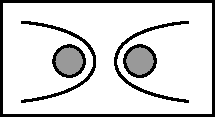
\includegraphics[width=150pt]{resources/chap_sep_count/normal.pdf}  
		\caption{Normal space}  
		\label{fig:normal}
	\end{figure}
	\begin{theorem}
		A space $X$ is a normal space iff for each open set $A\subseteq X$ and each closed set $B \subseteq A$, there exists an open set $C\supseteq B$ such that $C^-\subseteq A$.
	\end{theorem}
	
	\begin{theorem}[Urysohn]
		A space $X$ is a normal space iff for each two disjoint closed sets $A$ and each $B$, there exists a continuous function $f:X\mapsto I$ such that $f(A)=0$ and $f(B)=1$. Such a function is called a {\bf Urysohn function} for $A$ and $B$.
	\end{theorem}
	\begin{proof}
		Let $X$ be a normal space. We define $U_0=A$ and $U_1=X-B$. We have $U^-_0\subseteq U_1$. We define $U_{\frac n {2^m}}$ for $m>0, 0\leq n\leq 2^m$ by induction: with $U_a$ and $U_b$ ($a<b$) we define $U_{\frac {a+b}2}$ as an open set such that $U_a^-\subseteq U_{\frac {a+b}2}\subseteq U_{\frac {a+b}2}^-\subseteq U_b$. We define $f: X\mapsto \mathbb R$ as $f(x)=\inf\{r|x\in U_r\}$. It's easy to see that $f$ is continuous, $f(A)=0$ and $f(B)=1$.
	\end{proof}
	\begin{corollary}
		Every $T_4$ space is Tychonoff.
	\end{corollary}
	\begin{theorem}[Tietze]
		$X$ is a normal space iff for each closed sets $A\subseteq X$ and each continuous map $f:A\mapsto \mathbb R$, there is an extension of $f$ to all of $X$.
	\end{theorem}
	\begin{proof}
		We prove $\Rightarrow$. Since $[-1,1]$ is homeomorhpic to $\mathbb R$, we only need to prove that each continuous map $f:A\mapsto [-1,1]$ can be extended to all of $X$. Let $g_1=f$. We define $f_i$, $g_i$, $A_i$ and $B_i$ by induction:
		\begin{enumerate}
			\item $A_i=g_i^{-1}([\frac {2^{i-1}}{3^i},\frac {2^{i-1}}{3^{i-1}}])$ and $B_i=g_i^{-1}([-\frac {2^{i-1}}{3^{i-1}},-\frac {2^{i-1}}{3^i}])$.
			\item $f_i$ be the Urysohn function $X\mapsto[-\frac {2^{i-1}}{3^i},\frac {2^{i-1}}{3^i}]$ such that $f_i(A_i)=\frac {2^{i-1}}{3^i}$ and $f_i(B_i)=-\frac {2^{i-1}}{3^i}$.
			\item $g_{i+1}=g_i-f_i|_A$. It's easy to see that $g_{i+1}(x)\in [-\frac {2^i}{3^i},\frac {2^i}{3^i}]$
		\end{enumerate} 
		
		Since $\{f_i\}$ converges uniformly, $F=\sum_i f_i$ is continuous. It's easy to see that $F$ is an extension of $f$ to all of $X$.
	\end{proof}
	
	Note: we use $f_i$ to approach $f$ bit by bit while remaining controlled at $X-A$.

\begin{corollary}
	Let $X$ be a normal space. For each closed sets $A\subseteq X$, each open $U\supseteq A$, and each continuous map $f:A\mapsto \mathbb R$, there is an extension of $f$ to all of $X$ such that $supp(f)\subseteq U$.
\end{corollary}	
	
	
\begin{theorem}
	The closed subspace of a normal$/T_4$ is normal$/T_4$.
\end{theorem}
	
\begin{definition}
	A space $X$ is called {\bf completely normal} each subspace of $X$ is normal. A $T_1$ completely normal space is called a $T_5$ space.
\end{definition}

\begin{theorem}
	A space $X$ is completely normal iff for each pair of subsets of $X$, named $A$ and $B$, such that $A\cap B^-=A^-\cap B=\emptyset$, there are two disjoint open sets that contain $A$ and $B$ respectively.
\end{theorem}
\begin{proof}
	Let $X$ be completely normal. Consider the open subspace $Y=X-A^-\cap B^-$. $A^-\cap Y$ and $B^-\cap Y$ are disjoint closed sets in $Y$, and are contained in disjoint open sets $A'$ and $B'$. $A'$ and $B'$ are disjoint open sets that contain $A$ and $B$ respectively.
	
	Let $X$ be a space that for each pair of subsets that satisfy the requirement in the theorem, there are two disjoint open sets that contain each of them respectively. For each subspace $S$ of $X$, and each disjoint closed sets $A$ and $B$ of $S$. In $X$, it's easy to see that $A\cap B^-=A^-\cap B=\emptyset$. So There are two disjoint open sets in $X$ that contain $A$ and $B$ respectively. So $S$ is normal.
\end{proof}
	
\begin{definition}
	A space $X$ is called {\bf perfectly normal} if for each pair of disjoint closed sets $A$ and $B$, there exists a continuous function $f:X\mapsto I$ such that $A=f^{-1}(0)$ and $B=f^{-1}(1)$. A $T_1$ perfectly normal space is called a $T_6$ space.
\end{definition}

\begin{theorem}
	A space $X$ is perfectly normal iff
	\begin{enumerate}
		\item for each closed set $A$, there exists a continuous function $f:X\mapsto I$ such that $A=f^{-1}(0)$;
		\item each closed set is a countable intersection of open sets.
	\end{enumerate}
\end{theorem}
\begin{proof}
	Clearly perfect normality $\rightarrow1\rightarrow2$.
	
	$2\rightarrow1$: Let $A=\cup_n U_n$ be a closed set with all $U_n$ open. For each $U_n$, define a Urysohn function $f_n:X\mapsto I$ such that $f_n(A)=0$ and $f_n(X-U_n)=1$. Define $f=\sum_nf_n/2^n$. Then $A=f^{-1}(0)$.
	
	$1\rightarrow$ perfect normality: Let $A$ and $B$ be two disjoint closed sets, and $A=f^{-1}(0)$ and $B=g^{-1}(0)$. Then $f/(f+g)$ works.
\end{proof}

\begin{theorem}
	The subspace of a perfectly normal space is perfectly normal. 
\end{theorem}
\begin{corollary}
	A perfectly normal space is completely normal. A completely normal space is normal.
\end{corollary}

\begin{lemma}
	Each pseudo-metric space is perfectly normal. Each metric space is $T_6$. $T_6\rightarrow T_5\rightarrow T_4$.
\end{lemma}

\section{Shrinking Lemma}

\begin{definition}
	Let $X$ be a space. A collection of subsets of $X$ is called {\bf locally finite} iff each $x\in X$ has a neighborhood that intersects only finitely may of the sets in the collection.  A collection of subsets of $X$ is called {\bf discrete} iff each $x\in X$ has a neighborhood that intersects at most one set in the collection.
\end{definition}

\begin{lemma}
	Let $X$ be a normal space with an open cover $(U_1,U_2)$. There exists an open set $V_1$ such that $V_1^-\subseteq U_1$ and $(V_1,U_2)$ covers $X$.
\end{lemma}
\begin{proof}
	$X-U_2$ and $X-U_1$ are disjoint closed sets, covered by open sets $V_1$ and $V_2$ respectively. $V_1$ is what we want.
\end{proof}

\begin{lemma}
	Let $X$ be a normal space with an open cover $(U_1,\dots,U_n)$. There exists an open cover $(V_1,\dots,V_n)$ such that $\forall i(V_i^-\subseteq U_i)$.
\end{lemma}
\begin{proof}
	By induction.
\end{proof}

\begin{lemma}
	Let $X$ be a normal space with a locally finite open cover $\{U_i\}_{i\in I}$. There exists an open cover $\{V_i\}_{i\in I}$ such that $\forall i\in I(V_i^-\subseteq U_i)$.
\end{lemma}
\begin{proof}
	We consider the set $S$ of pairs $(J,\mathcal V)$ where $J\subseteq I$ and $\mathcal V=\{V_i\}_{i\in I}$ is an open cover of $X$ such that
	\begin{enumerate}
		\item $i\in J\rightarrow V_i^-\subseteq U_i$;
		\item $i\not\in J\rightarrow V_i=U_i$.
	\end{enumerate}
	
	We equip the set $S$ with a partial order $(J_1,\mathcal V_1)\leq (J_2,\mathcal V_2)\leftrightarrow (J_1\subseteq J_2)\wedge(\forall i\in J_1 (V_{1i}=V_{2i}))$. It's easy to see that each chain has a maximal element. By Zorn's lemma, there's a maximal element $(J,\mathcal V)$. It's easy to see that $J=I$.
\end{proof}
	
\section{Countability}
\begin{definition}
	A space is called {\bf 1st countable} if each point has a countable local base.
\end{definition}

\begin{example}
	A pseudo-metric space is 1st countable.
\end{example}

\begin{lemma}
	Let $X$ be a 1st countable space. At each $x\in X$ we can find an countable local base $\{B_n|n\in\mathbb N\}$ such that $B_1\supseteq B_2\supseteq\cdots$.
\end{lemma}

\begin{corollary}
	A 1st countable space is a Fr\'echet-Urysohn space, and hence a sequential space.
\end{corollary}

\begin{theorem}
	A 1st countable space is a Hausdorff space iff each sequence only converges to at most one point.
\end{theorem}

\begin{lemma}
	A product of 1st countable spaces is 1st countable iff each factor space is 1st countable and all but countably many of the factor spaces are trivial.
	\label{lem:1count_prod}
\end{lemma}
\begin{proof}
	Let $\prod_{\alpha\in A} X_\alpha$ be 1st countable. Then clearly each $X_\alpha$ is 1st countable. Let $A'=\{\alpha\in A|X_\alpha$ is non-trivial$\}$. We can find $(x_\alpha)\in\prod_{\alpha\in A} X_\alpha$ such that $\forall \alpha\in A'$ there exists a non-trivial open set $U_\alpha\ni x_\alpha$. Let $\mathcal B$ be a local base at $(x_\alpha)$. For each $B\in \mathcal B$ we can find $B\supseteq \prod_{\alpha\in A_B}U(B)_\alpha\times\prod_{\alpha\not\in A_B}X_\alpha\ni x$, where $U(B)_\alpha$ is an non-trivial open set in $X_\alpha$. Clearly $A_B$ is finite. Let $A''=\bigcup_B A_B$. $A''$ is countable. It's easy to see that $A''\subseteq A'$. If $A''\neq A'$, let $\beta\in (A'-A'')$, and $U_\beta$ be a non-trivial open set in $X_\beta$. Then $U_\beta\times\prod_{\alpha\in A,\alpha\neq\beta}X_\alpha$ is an open set in $\prod_{\alpha\in A} X_\alpha$ but contains no base in $\mathcal B$, a contradiction. So  $A'=A''$ is (at most) countable.
\end{proof}
	
\begin{definition}
	A space is called {\bf 2nd countable} if it has a countable base. Clearly a 2nd countable space is a 1st countable space
\end{definition}
\begin{definition}
	A space is called {\bf separable} if it has a countable dense subset.
\end{definition}
\begin{definition}
	Let $X$ be a topological space. A family $\mathcal A$ of subsets of $X$ is called a {\bf cover} of $X$ if the union of $\mathcal A$ is $X$. A subfamily of $\mathcal A$ is called a {\bf subcover} if its union is $X$. An {\bf open cover} is a cover of open sets.
\end{definition}
\begin{definition}
	A space is called a {\bf Lindel\"of space} if each open cover of it has a countable subcover.
\end{definition}
\begin{theorem}
	A regular Lindel\"of space is normal.
\end{theorem}
\begin{proof}
	Let $A$ and $B$ be two disjoint closed sets in a regular Lindel\"of space $X$. For each $a\in A$ we choose an open set (using AC) $U_a\ni a$ such that $U_a^-\cap B=\emptyset$. Since $\{U_a\}$ covers $A$, we can find a countable (assumed to be infinite) subcover $\{U_n|n\in\mathbb N\}$, such that $A\subseteq \bigcup U_n$. Similarly we have $B\subseteq \bigcup V_n$. However, at present, $(\bigcup U_n)\cap(\bigcup V_n)\neq\emptyset$.
	
	We can define $U_n'$ and $V_n'$ by induction:
	\begin{enumerate}
		\item $U_i'=U_i-(\bigcup_{n<i}V_i')^-$
		\item $V_i'=V_i-(\bigcup_{n\leq i}U_i')^-$
	\end{enumerate}
	It's easy to see that $\bigcup U_n$ and $\bigcup V_n$ and disjoint open sets that contains $A$ and $B$ respectively.
\end{proof}

\begin{theorem}
	A 2nd countable space is a separable Lindel\"of space.
\end{theorem}
\begin{theorem}
	Let $X$ be a pseudometric space. The following are equivalent:
	\begin{enumerate}
		\item $X$ is 2nd countable.
		\item $X$ is Lindel\"of.
		\item $X$ is separable.
	\end{enumerate}
\end{theorem}
\chapter{Compactness}
\section{Compact Space}

\begin{definition}
	A topological space is a {\bf compact space} iff each open cover has a finite subcover. 
\end{definition}

\begin{lemma}
	A topological space is a compact space iff each family of closed sets with empty intersection has a finite subfamily with empty intersection. 
\end{lemma}

\begin{theorem}
	Let $X$ be a topological space. The following statements are equivalent:
	\begin{enumerate}
		\item $X$ is compact
		\item Each filter (or equivalently each net) in $X$ has a cluster point.
		\item Each filter (or equivalently each net) in $X$ has a convergent finer filter(subnet).
		\item Each ultrafilter (or equivalently each ultranet) in $X$ converges.
	\end{enumerate}
	\label{thm:compact_cluster}
\end{theorem}
\begin{proof}

	$1\Leftrightarrow2$:
	
	$X$ is compact
	
	iff $\forall$ family of closed sets $\mathcal F$ such that $\bigcap_{F\in\mathcal F}F=\emptyset$ there's a finite subfamily $\mathcal F'$ such that $\bigcap_{F\in\mathcal F'}F=\emptyset$
	
	iff $\forall$ family $\mathcal F$ such that $\bigcap_{F\in\mathcal F}F^-=\emptyset$ there's a finite subfamily $\mathcal F'$ such that $\bigcap_{F\in\mathcal F'}F^-=\emptyset$
	
	iff $\forall$ family $\mathcal F$ such that $\bigcap_{F\in\mathcal F}F^-=\emptyset$ is not a filter subbase
	
	iff $\forall$ filter $\mathcal F(\bigcap_{F\in\mathcal F}F^-\neq\emptyset)$

	It's easy to see that $2\Leftrightarrow 3\Leftrightarrow 4$.
\end{proof}

\begin{theorem}
	A compact subset of a Hausdorff space is closed.
\end{theorem}

\begin{theorem}
	A closed subset of a compact space is compact.
\end{theorem}

\begin{theorem}
	The continuous image of a compact space is compact.
\end{theorem}

\begin{theorem}
	A non-empty product space is compact iff each factor space is compact.
\end{theorem}
\begin{proof}
	Let $X=\prod_\alpha X_\alpha$. If each $X_\alpha$ is compact. Let $\{(x_\alpha^i)|i\in \Lambda\}$ be a supernet in $X$. It's easy to see that for each $\alpha$, $\{x_\alpha^i|i\in \Lambda\}$ is a supernet in $X_\alpha$, and it converges, say to $x_\alpha$. It's easy to see that $\{(x_\alpha^i)|i\in \Lambda\}$ converges to $(x_\alpha)$.
\end{proof}

\begin{theorem}
	$I$ is compact with usual topology.
\end{theorem}
\begin{proof}
	For each open cover $\mathcal U$ of $I$, let $S=\{x|[0,x]$ is covered by finite elements of $\mathcal U\}$. If $\sup S<1$, then let $\sup S\in (a,b)\subseteq U\in\mathcal U$, where $\sup S<b$. Then $b\in S$, a contradiction.
\end{proof}

\begin{corollary}
	A subspace of $\mathbb R^n$ with usual topology is compact iff it's closed and bounded.
\end{corollary}

\begin{lemma}
	Disjoint compact subsets of a Hausdorff space can be separated by disjoint open sets.
\end{lemma}

\begin{corollary}
	A compact Hausdorff space $X$ is a $T_4$ space.
\end{corollary}

\begin{definition}
	A topological space is a {\bf countably compact space} iff each countable open cover has a finite subcover. Clearly a space is compact iff it's Lindel\"of and countably compact.
\end{definition}

\begin{lemma}
	A topological space is a countably compact space iff each countable family of closed sets with empty intersection has a finite subfamily with empty intersection. 
\end{lemma}

\begin{theorem}
	A closed subset of a countably compact space is countably compact.
\end{theorem}

\begin{theorem}
	A continuous real-valued function on a countable compact space is bounded.
\end{theorem}

\begin{theorem}
	A space $X$ is countably compact iff each sequence in $X$ has a cluster point.
\end{theorem}
We prove this theorem following the spirit of the proof of Thm. \ref{thm:compact_cluster}.
\begin{proof}
	$\Rightarrow$: Let $\{x_n\}$ be a sequence. For each $n\in\mathbb N$, we define $S_n=\{x_m|m\geq n\}^-$. If $\bigcap_n\{S_n|n\in\mathbb N\}=\emptyset$, then $\exists n_0(\bigcap_n\{S_n|n<n_0\}=\emptyset)$. That means $\{x_m|m\geq n_0\}^-=\emptyset$, which is impossible. So $\bigcap_n S_n\neq \emptyset$. Any $x\in \bigcap_n S_n$ is a cluster point of $\{x_n\}$.
	
	$\Leftarrow$: Let $\{U_n|n\in \mathbb N\}$ be a family of closed sets such that  $\bigcap_n\{U_n|n\in\mathbb N\}=\emptyset$. If $(\forall n\in\mathbb N) \bigcap_{m\leq n}U_m\neq\emptyset$, we can always choose $x_n\in \bigcap_{m\leq n}U_m$. The sequence $\{x_n\}$ has a cluster point $a$. Let $a\not\in U_m$, then $\forall k>m(x_k\in U_m)$, a contradiction.
\end{proof}

\begin{definition}
	A topological space $X$ is a {\bf sequentially compact space} iff each sequence in $X$ has a convergent subsequence.
\end{definition}

\begin{definition}
	A topological space $X$ is a {\bf limit-point compact space} iff each infinite subset in $X$ has a limit point.
\end{definition}

\begin{definition}
	A space is {\bf locally compact} iff each point has a compact neighborhood.
\end{definition}

\begin{theorem}
	In a locally compact Hausdorff space, each point has a compact neighborhood base.
\end{theorem}
\begin{proof}
	Let $x$ be a point with a compact neighborhood $U$ and a local base $\mathcal N_x$. $U$ is a compact Hausdorff space, so it's $T_3$. For each $N\in \mathcal N_x$, $N\cap U$ is an open neighborhood of $x$, which contains a closed neighborhood $N'$ of $x$ in $U$, which is compact. It's easy to see all $N'$s form a compact neighborhood base.
\end{proof}

\section{Relationship between Different Compact Conditions}

\begin{theorem}
	Every sequentially compact space is countable compact.
\end{theorem}
\begin{proof}
	Each sequence has a cluster point that a subsequence converges to.
\end{proof}

\begin{theorem}
	Every countable compact space is limit-point compact.
\end{theorem}
\begin{proof}
	We can construct a sequence in a infinite subset such that any two elements are different. This sequence converges to a limit point of the subset.
\end{proof}

\begin{theorem}
	A $T_1$ limit-point compact space is countable compact.
\end{theorem}
\begin{proof}
	For each sequence with infinite elements, we have a limit point. Since the space is $T_1$, the limit point has a neighborhood that excludes the first $n$ points of the sequence for each $n$. So the limit point is a cluster point of the sequence.
\end{proof}

\begin{theorem}
	A sequential limit-point compact space is sequentially compact.
\end{theorem}
\begin{proof}
	Let $(x_n)$ be a sequence with infinite elements. Let $A=\{x_n|n\in \mathbb N\}$ with limit point $x$. Clearly $A-\{x\}$ is not closed. So there's a sequence $(y_n)$ in $A-\{x\}$ that converges. Then it's easy to find a subsequence of $(x_n)$ that converges.
\end{proof}

\begin{theorem}
	A Lindel\"of countable compact space is compact.
\end{theorem}

\begin{lemma}
	Every sequentially compact metric space is 2nd countable.
\end{lemma}
\begin{proof}
	Let $X$ be a sequentially compact metric space. For each $n\in \mathbb N$, pick $x_1^{[n]}\in X$, then pick $x_2^{[n]}\in (X-B(x_1^{[n]},1/n))$ if possible, then pick $x_3^{[n]}\in (X-B(x_1^{[n]},1/n)\cup B(x_2^{[n]},1/n))$ if possible \dots For each $n$, this process must stop in $M_n$ steps. Otherwise we have a sequence $(x_i^{[n]})$, which has a cluster point $x^{[n]}$. $B(x^{[n]},1/n)$ contains some elements in $(x_i^{[n]})$, say $x_m^{[n]}$. Thus $\rho(x^{[n]},x_m^{[n]})<1/n$. Thus $B(x^{[n]},1/n-\rho(x^{[n]},x_m^{[n]}))$ contains no element in $(x_i^{[n]})$, a contradiction. It's easy to see that $\{B(x_i^{[n]},1/n)|n\in\mathbb N,i\leq M_n\}$ forms a countable base.
\end{proof}

The relationship between different compact conditions is shown in Fig. \ref{fig:compact_relation}.

\begin{figure}[htb!]
	\centering  
	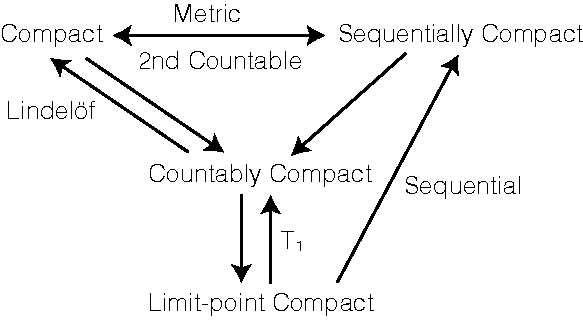
\includegraphics[width=0.5\textwidth ]{resources/chap_compact/compactness.pdf}  
	\caption{Relationship between different compact conditions.}
	\label{fig:compact_relation}
\end{figure}

\section{Compactification}

\begin{definition}
	Let $X$ be a topological space. A {\bf compactification}, written as $(Y,f)$, is an embedding $f$ of $X$ to a compact space $Y$ such that $f(X)$ is dense in $Y$. If $Y$ is further Hausdorff, the compactification is called a {\bf Hausdorff compactification}.
\end{definition}

\begin{lemma}
	A space has a Hausdorff compactification iff it's Tychonoff.
\end{lemma}

\begin{definition}
	Let $X$ be a topological space. Let $X'=X\cup\{\infty\}$ ($\infty\not\in X$). In $X'$, let $\{X'-T| T$ is compact in $X\}$ be a neighborhood base at $\infty$ and the neighborhood base at any $x\in X$ is identical to $X$. This gives us a topology of $X'$, with which $X'$ is a compact space. This process is illustrated in Fig. \ref{fig:1p_compact}. $X'$ is called the {\bf Alexandroff extension} of $X$.
\end{definition}

\begin{figure}[htb!]
	\centering  
	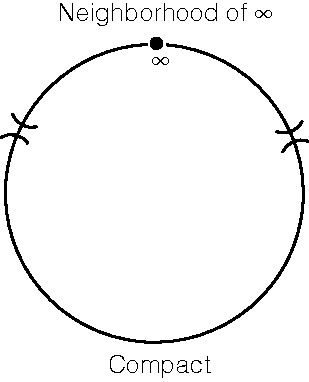
\includegraphics[width=0.27\textwidth ]{resources/chap_compact/one-point-comp.pdf}  
	\caption{Illustration of Alexandroff extension.}
	\label{fig:1p_compact}
\end{figure}

\begin{lemma}
	 Let $X$ be a locally compact and Hausdorff but not compact space. Let $X'$ be the Alexandroff extension of $X$. Then $(X',\iota)$ is a Hausdorff compactification, called {\bf one-point compactification}.
\end{lemma}

\begin{corollary}
	A locally compact Hausdorff space is Tychonoff.
\end{corollary}

\begin{definition}
	Let $X$ be a Tychonoff space.  As in Col. \ref{col:tych_embed}, we have an embedding $e:X\mapsto \prod_{f\in C^*(X)} I_f$, where $e$ is the evaluation map induced by $C^*(X)$. The map $X\mapsto e(X)^-$ is a Hausdorff compactification, called the {\bf Stone-\v Cech compactification}. The space $e(X)^-$ is usually denoted by $\beta X$.
\end{definition}

\begin{theorem}
	Let $K$ be a compact Hausdorff space, $X$ be a Tychonoff space, $(\beta X,e)$ be the Stone-\v Cech compactification of $X$. For each continuous map $f:X\mapsto K$ be continuous, there's a unique continuous map $F:\beta X\mapsto K$ such that $F\circ e=f$.
\end{theorem}

\begin{proof}
	We already have an embedding $e:X\rightarrow \prod_{g\in C^*(X)}I_g$. Similarly we can construct an embedding $e':K\rightarrow \prod_{g\in C^*(K)}I_g$. Using $f:X\mapsto K$, can construct a continuous function $T_f:\prod_{g\in C^*(X)}I_g\mapsto\prod_{g\in C^*(K)}I_g$ by
	\begin{equation}
		(T_f(a))_g=(a)_{g\circ f},\ \forall g\in  C^*(K)
	\end{equation}
	
	Since $\forall x\in X\forall g\in  C^*(K)$, $(T_f(e(x)))_g=(e(x))_{g\circ f}=g(f(x))$. We have $T_f\circ e=e'\circ f$. That is, the following diagram commutes.
	\[
	\begin{tikzcd}
		\prod_{g\in C^*(X)}I_g \arrow{r}{T_f}  & \prod_{g\in C^*(K)}I_g\\
		X \arrow{r}{f} \arrow[swap]{u}{e}& K \arrow{u}{e'} 
	\end{tikzcd}
	\]
	
	Clearly $T_f(e(X))\subseteq e'(K)$. Thus $T_f(\beta X)\subseteq e'(K)^-=e'(K)$. We define $F:\beta X\mapsto K$ as $F=e'^{-1}\circ T_f|_{\beta X}$. It's easy to see that $F\circ e=f$.
	
	For uniqueness, use Thm. \ref{thm:Haus_dense}.
\end{proof}

\begin{definition}
	Let $X$ be Tychonoff space, $\tilde X$ be the class of all compactifications of $X$. We define a equivalence relation $(K_1,h_1)\sim(K_2,h_2)$ iff there is an homeomorphism $f:K_1\mapsto K_2$ such that $f\circ h_1=h_2$. Let $[\tilde X]$ be the resulting equivalent classes. We can define a binary relation on $[\tilde X]$: $[(K_1,h_1)]\leq[(K_2,h_2)]$ iff there's a continuous function $F:K_2\mapsto K_1$ such that $F\circ h_2=h_1$.
\end{definition}   
\begin{lemma}
	The binary relation $\leq$ we just defined is a well-defined partial order.
\end{lemma}
\begin{proof}
	Let $[(K_1,h_1)],[(K_2,h_2)]\in[\tilde X]$, $[(K_1,h_1)]\leq[(K_2,h_2)]$ with continuous function $F:K_2\mapsto K_1$, and $[(K_2,h_2)]\leq[(K_1,h_1)]$ with continuous function $G:K_1\mapsto K_2$. We have $G\circ F\circ h_2=G\circ h_1=h_2$. So $G\circ F|_{h_2(X)}=1_{h_2(X)}$. Since $h_2(X)$ is dense in $K_2$, we have $G\circ F=1$. Similarly  $F\circ G=1$. So $F=G^{-1}$ is a homeomorphism. So $[(K_1,h_1)]=[(K_2,h_2)]$.
\end{proof}
\begin{theorem}
	Let $X$ be Tychonoff space. The Stone-\v Cech compactification $[(\beta X,e)]$ is the maximal element in $[\tilde X]$.
\end{theorem}

\section{Paracompactness}

\begin{definition}
	Let $\mathcal U$ and $\mathcal V$ be two covers of $X$. $\mathcal V$ is a {\bf refinement} of $\mathcal U$ iff $(\forall V\in \mathcal V)(\exists U\in\mathcal U)V\subseteq U$.
\end{definition}

\begin{definition}
	Let $X$ be a space. A collection of subsets of $X$ is {\bf $\sigma$-locally finite} iff it is the union of a countable family of locally finite collections of subsets of $X$. A collections of subsets of $X$ is {\bf $\sigma$-discrete} iff it is the union of a countable family of discrete collections of subsets of $X$.
\end{definition}

\begin{definition}
	A Hausdorff space $X$ is {\bf paracompact} iff each open cover of $X$ has an open locally finite refinement.
\end{definition}

\begin{theorem}[Michael]
	Let $X$ be a $T_3$ space. The following are equivalent:
	\begin{enumerate}
		\item $X$ is paracompact.
		\item Each open cover of $X$ has an open $\sigma$-locally finite refinement.
		\item Each open cover of $X$ has a locally finite refinement.
		\item Each open cover of $X$ has a closed locally finite refinement.
	\end{enumerate}
\end{theorem}
\begin{proof}
	$2\rightarrow 3$: Let $\mathcal U$ be an open cover of $X$. Let $\mathcal V=\bigcup_n \mathcal V_n$ be an open $\sigma$-locally finite refinement. Let $A_n=\bigcup\mathcal V_n-\bigcup_{m<n}(\bigcup\mathcal V_m)$. Then $\{A_n|n\in\mathbb N\}$ is a locally finite cover of $X$. It's easy to see that $\{V_n\cap A_n|V_n\in\mathcal V_n,n\in\mathbb N\}$ is a locally finite refinement of $\mathcal U$.
	
	$3\rightarrow 4$: Let $\mathcal U$ be an open cover of $X$. For each $x\in X$, chose a $U_x\in\mathcal U$ such that $x\in U_x$. Choose an open set $V_x$ such that $x\in V_x\subseteq V_x^-\subseteq U_x$. Then $\{V_x|x\in X\}$ is a open refinement of $\mathcal U$, and has a locally finite refinement $\mathcal S$. It's easy to see that $\{S^-|X\in\mathcal S\}$ is a closed locally finite refinement of $\mathcal U$.
	
	$4\rightarrow 1$: Let $\mathcal U$ be an open cover of $X$, which has a closed locally finite refinement $\mathcal V$. For each $x\in X$, we can choose $W_x$ that intersects with finitely many of elements in $\mathcal V$. This forms an open cover $\mathcal W=\{W_x|x\in X\}$, which has a closed locally finite refinement $\mathcal A$. For each $V\in\mathcal V$, let $V^*=X-\bigcup\{A\in\mathcal A|A\cap V=\emptyset\}$. Clearly $\{V^*|V\in\mathcal V\}$ is an open  refinement. Furthermore, for each $x\in X$, there's a neighborhood $N$ of $x$ that only intersects with finitely many members of $\mathcal A$. Since each element in $\mathcal A$ only intersects with finitely many members of $\mathcal V$. We see that $N$ only intersects with finitely many $V^*$s. So $\{V^*|V\in\mathcal V\}$ is an open locally finite refinement of $\mathcal U$. 
\end{proof}

\begin{theorem}[Stone]
	Every pseudometric space is paracompact.
	\label{thm:paracomp}
\end{theorem}
\begin{proof}
	Let $\mathcal U$ be an open cover of the metric space $X$. For each $n\in\mathbb N$ and $U\in\mathcal U$, let $U_n=\{x\in U|\rho(x,X-U)\geq 1/2^n\}$. Let $\leq$ be a well-ordering of $\mathcal U$. Let $U^*_n=U_n-\bigcup_{V<U}V_{n+1}$, as shown in Fig. \ref{fig:paracompact}. It's easy to see that $\rho(U^*_n,V^*_n)\geq 1/2^{n+1}$ for each $U\neq V\in\mathcal U$. Let $U_n^\sim=\{x\in U|\rho(x,U_n^*)< 1/2^{n+3}\}$. $\bigcup_n\{U_n^\sim|U\in\mathcal U\}$ is a $\sigma$-discrete open refinement of $\mathcal U$.
\end{proof}
\begin{figure}[htb!]
	\centering  
	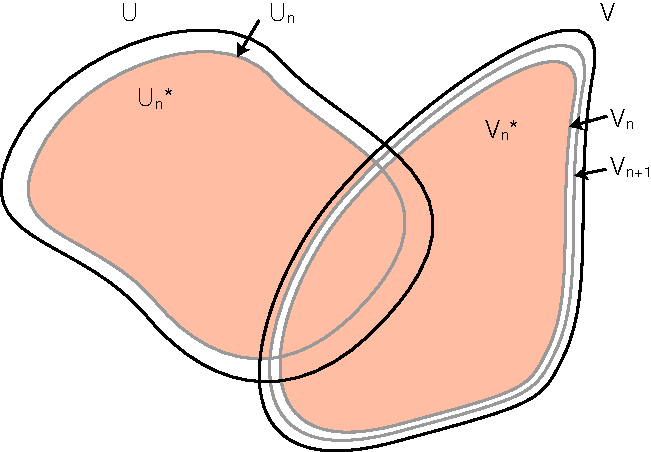
\includegraphics[width=0.5\textwidth ]{resources/chap_compact/paracompact.pdf}  
	\caption{$U^*_n$ and $V^*_n$, where $V<U$.}
	\label{fig:paracompact}
\end{figure}

\begin{theorem}
	A closed subspace of a paracompact space is paracompact.
\end{theorem}

\begin{theorem}
	A Hausdorff paracompact space is normal.
\end{theorem}
\begin{proof}
	Firstly, we prove the regularity. Let $X$ be a Hausdorff paracompact space, $x\in X$ and $A$ be a closed set not containing $x$. For each $a\in A$, we have two disjoint open sets $U_a\ni x$ and $V_a\ni a$. $\{X-A\}\cup\{V_a|a\in A\}$ is an open cover of $X$. It has an open locally finite refinement $\mathcal V$. Discarding the open sets contained in $X-A$, we have an open locally finite cover $\mathcal V'$ of $A$. Let $N$ be an open neighborhood of $x$ disjoint from $A$ that intersects with finitely members of $\mathcal V'$. Since each member in $\mathcal V'$ doesn't contain $x$. We can further shrink $N$ to $N'$ which is disjoint from all elements of $\mathcal V'$. Then $\bigcup\mathcal V'$ is an open set that contains $A$ and is disjoint from $N'$.
	
	Secondly, we prove the normality. Let $X$ be a Hausdorff paracompact space, $A$ and $B$ be two disjoint closed sets. Mimicking the first part, we have an open locally finite cover $\mathcal U$ of $A$, of which each element is disjoint from $B$. Similarly, for each $b\in B$ we have an open neighborhood $V_b$ disjoint from each member of $\mathcal U$. Then $\bigcup\mathcal V'$ and $\bigcup V_b$ are disjoint open sets that contains $A$ and $B$ respectively.
\end{proof}

\section{Partition of Unity}
\begin{definition}
	Let $X$ be a topological space, and let $\{U_i\}_{i\in I}$ be an open cover. Then a {\bf partition of unity} subordinate to the cover is a set $\{f_i\}_{i\in I}$ of continuous functions $f_i:X\mapsto I$ such that 
	\begin{enumerate}
		\item $(\forall i\in I)supp(f_i)\subseteq U_i$;
		\item $\{supp(f_i)\}_{i\in I}$ is a locally finite cover;
		\item $(\forall x\in X)\sum_{i\in I}f_i(x)=1$.
	\end{enumerate}
	where $supp(f_i)=(f_i^{-1}((0,1]))^-$.
\end{definition}

\begin{lemma}
	Let $X$ be a paracompact space with open cover $\mathcal U=\{U_i\}_{i\in I}$. Then $\mathcal U$ has a locally finite refinement $\{V_i\}_{i\in I}$ such that $(\forall i\in I)V_i\subseteq U_i$.
\end{lemma}
\begin{proof}
	Let $\{W_i\}_{i\in J}$ be a locally finite refinement of $\mathcal U$. Let $\phi: J\mapsto I$ be a choice function $W_i\subseteq U_{\phi(i)}$. Let $V_i=\bigcup_{j\in\phi^{-1}(i)}V_j$. Then $\{V_i\}_{i\in I}$ is a locally finite refinement.
\end{proof}

\begin{lemma}
	Let $X$ be a paracompact Hausdorff space. For each open cover $\{U_i\}_{i\in I}$, there is a subordinate partition of unity.
\end{lemma}
\begin{proof}
	Let $\{V_i\}_{i\in I}$ be a locally finite refinement of $\{U_i\}_{i\in I}$ such that $(\forall i\in I)V_i\subseteq U_i$. By shrinking lemma, we have covers $\{W_i\}_{i\in I}$ and $\{T_i\}_{i\in I}$ such that $(\forall i\in I)T_i\subseteq T_i^-\subseteq W_i\subseteq W_i^-\subseteq V_i$. Let $f_i$ be a Urysohn function for $T_i^-$ and $X-W_i$, such $f_i(T_i^-)=1$ and $f_i(X-W_i)=0$. So $(\forall i\in I)T_i\subseteq supp(f_i)\subseteq V_i$. For each $x\in X$ let $f(x)=\sum_if_i(x)$. It's easy to see that $f_i$ is well-defined, non-zero and continuous. Let $f_i'=f_i/f$. Then $\{f_i'\}$ is a partition of unity.
\end{proof}

\chapter{Connectedness}

\section{Connectedness}
\begin{definition}
	A space $X$ is {\bf disconnected} if there's two disjoint nonempty open sets $U$ and $V$ such that $X=U\cup V$. A space is {\bf connected} if it's not disconnected.
\end{definition}

\begin{lemma}
	The continuous image of a connected space is connected.
\end{lemma}

\begin{lemma}
	Let $S\subseteq X$ be connected. Then $S^-$ is connected.
\end{lemma}

\begin{definition}
	Two set $A$ and $B$ in $X$ are {\bf mutually separated} iff $A^-\cap B=A\cap B^-=\emptyset$.
\end{definition}

\begin{lemma}
	Let $A$ and $B$ be mutually separated sets, and $C\subseteq A\cup B$ be a connected set. Then $C\subseteq A$ or $C\subseteq B$.
\end{lemma}

\begin{lemma}
	Let $\mathcal C$ be a family of connected subsets of $X$. $\bigcup \mathcal C$ is connected if no two members of $\mathcal C$ are mutually separated.
\end{lemma}
\begin{proof}
	Let $\bigcup \mathcal C=A\cap B$ be disconnected, where $A$ and $B$ are nonempty open sets in $\bigcup \mathcal C$. Clearly $A$ and $B$ are mutually disjoint in $\bigcup \mathcal C$. So $(\forall C\in\mathcal C)C\in A\vee C\in B$. Each $C$ in $A$ and each $C'$ in $B$ are mutually disjoint.
\end{proof}

\begin{corollary}
	Let $\{C_n|n\in\mathbb N\}$ be a family of connected subsets of $X$. For each $n$, $C_n$ and $C_{n+1}$ are not mutually separated. Then $\bigcup_nC_n$ is connected.
\end{corollary}
\begin{proof}
	Clearly for each $N$, $\bigcup_{n<N}C_n$ is connected.
\end{proof}

\begin{lemma}
	A product space is connected iff each factor space is connected.
\end{lemma}
\begin{proof}
	Let $X=\prod_{\alpha\in A} X_\alpha$ be disconnected. Let $X=A\cup B$ where $A$ and $B$. Let $U$ and $V$ be two basic open sets in $A$ and $B$ respectively. We have a finite subset $A'=\{\alpha_n|0<n\leq N\}\subseteq A$ such that $U=\prod_{\alpha\in A'}U_\alpha\times\prod_{\alpha\in (A-A')}X_\alpha$ and $V=\prod_{\alpha\in A'}V_\alpha\times\prod_{\alpha\in (A-A')}X_\alpha$. We can find $u\in U$ and $v\in V$ such that $u_\alpha=v_\alpha$ for $\alpha\in (A-A')$. We define $u_n\in X$ by $u_{n,\alpha_m}=u_{\alpha_m}$ for $m<n$, $u_{n,\alpha_m}=v_{\alpha_m}$ for $m\geq n$ and  $u_\alpha=v_\alpha$ for $\alpha\in (A-A')$. Clearly $u_1=v$ and $u_{N+1}=u$. Let $u_m\in B$ and $u_{m+1}\in A$. Let $L=\{x\in X|x_{n,\alpha_i}=u_{\alpha_i}$ for $i<m$ and $x_{n,\alpha_i}=v_{\alpha_i} $ for $i>m$ and $x_\alpha=v_\alpha$ for $\alpha\in (A-A')\}$. Clearly $u_{m+1}\in A\cup L\neq\emptyset$ and $u_m\in B\cup L\neq\emptyset$. So $L$ is disconnected. And $L$ is homeomorphic to $X_{\alpha_m}$. So there exists a disconnected factor space.
\end{proof}

\begin{definition}
	Let $X$ be a space and $x\in X$. The {\bf component} of $x$ is the union of all connected sets that contain $x$.
\end{definition}

\begin{lemma}
	The {\bf component} of $x$ is connected and closed.
\end{lemma}

\begin{definition}
	Let $X$ be a space. The {\bf components} of $X$ is the family of sets that are components of some $x\in X$.
\end{definition}

\begin{lemma}
	The {\bf components} of $X$ is a disjoint closed cover of $X$.
\end{lemma}


\begin{definition}
	A space $X$ is {\bf locally connected} iff each point has a neighborhood base consisting of connected sets.
\end{definition}

\begin{lemma}
	$X$ is locally connected iff each component of each open set is open.
\end{lemma}

\begin{corollary}
	The components of a locally connected space are open and closed.
\end{corollary}

\section{Path-connectedness}

\begin{definition}
	Let $X$ be a space and $x,y\in X$. $x$ and $y$ are {\bf connected by a path} if there's a continuous function $f:I\mapsto X$ such that $f(0)=x$ and $f(1)=y$.
\end{definition}

\begin{definition}
	A space is {\bf path-connected} if any two points are connected by a path.
\end{definition}

\begin{lemma}
	Every path-connected space is connected.
\end{lemma}

\begin{definition}
	A space $X$ is {\bf locally path-connected} iff each point has a neighborhood base consisting of path-connected sets.
\end{definition}

\begin{theorem}
	A connected, locally path-connected space $X$ is path-connected.
\end{theorem}
\begin{proof}
	Let $x\in X$, and $B_x=\{y\in X| x$ and $y$ are connected by a path$\}$. It can be shown that $B_x$ is both open and closed. So $B_x=X$.
\end{proof}

\begin{example}
	A path-connected space need not be locally path-connected. A counter example is the {\bf comb space}. The comb space is a subspace of $I\times I$, defined by $C=\{(x,y)\subseteq I\times I|x=0\vee y=0\vee 1/x\in\mathbb N\}$. $X$ is path-connected, but not locally path-connected at $(0,0.5)$.
\end{example}

\chapter{Metrizable Spaces}

\section{Metrization}

\begin{lemma}
	Let $X$ be a metric space with metric $\rho$. Let $\rho'=\min(\rho,1)$. Then the metric space induced by $\rho'$ is the same as $X$.
\end{lemma}

\begin{lemma}
	A nonempty product space $\prod_\alpha M_\alpha$ is metrizable iff each $M_\alpha$ is metrizable and $M_\alpha$ is a single point for all but a countable set of indices.
\end{lemma}
\begin{proof}
	$\Rightarrow$: Use Lem. \ref{lem:1count_prod}.
	
	$\Leftarrow$: Let $\prod_i M_i$ be a product of countably many non-trivial metric spaces, and let $\rho_i\leq 1$ be a metric of $X_i$. We define a metric $\rho=\sum\rho_i/2^i$, which induce a topology with the base $\{B(x,\epsilon)|x\in X,\epsilon<1\}$. The base of the product topology is $\{\prod_{i\leq n}B_i(x,\epsilon_i)\times\prod_{i>n}X_i|x\in X,\epsilon_i<1\}$. These two bases give the same topology, since given $B=\prod_{i\leq n}B_i(x,\epsilon_i)\times\prod_{i>n}X_i$ we have $B(x,\epsilon)\subseteq B$ if $\epsilon<\epsilon_i/2^i$ for all $i\leq n$, and given $B(x,\epsilon)$ we have $\prod_{i\leq n}B_i(x,\epsilon/2n)\times\prod_{i>n}X_i\subseteq B(x,\epsilon)$ if $\sum_{i>n}1/2^i<\epsilon/2$.
\end{proof}
\begin{corollary}
	The space $I^{\omega}$ with product topology is metrizable.
\end{corollary}

\begin{theorem}[Urysohn]
	A 2nd countable Tychonoff space $X$ is metrizable.
\end{theorem}
\begin{proof}
	Let $\{B_n\}$ be a countable base and $x_n\in B_n$. Let $f_n:X\mapsto I$ be a map such that $f(x_n)=1$ and $f(X-B_n)=0$. Using Thm. \ref{thm:weak_embed}, we see $X$ can be embedded in $I^{\omega}$.
\end{proof}

\begin{theorem}
	A space is metrizable iff it's $T_3$ and has a $\sigma$-locally finite base.
\end{theorem}

\begin{proof}
	Let $X$ be a metric space with metric $\rho$. For each $n\in \mathbb N$, let $\mathcal B_n=\{B(x,1/n)|x\in X\}$ be an open cover of $X$. From Thm. \ref{thm:paracomp}, $\mathcal B_n$ has a locally finite refinement. So $X$ has a $\sigma$-locally finite base.
\end{proof}

\section{Complete Metric Spaces}
\begin{theorem}
	Every metric space $M$ can be isometrically embedded as a dense subset of a complete space.
\end{theorem}
\begin{proof}
	Let $\mathcal M$ be the set of all Cauchy sequences in $M$. We define a pseudometric on $\mathcal M$ as
	\begin{equation}
		\tilde\rho(\{x_n\},\{y_n\})=\lim_{n\rightarrow\infty}\rho(x_n,y_n)
	\end{equation}
	Since $\{\rho(x_n,y_n)\}$ is a Cauchy sequence in $\mathbb R$ ($|\rho(x_n,y_n)-\rho(x_m,y_m)|\leq\rho(x_n,x_m)+\rho(y_n,y_m)$), the limit always exists. It's easy to see $\mathcal M$ is a pseudometric space. It induce a metric space $\mathcal M^*$ as in Lem. \ref{lem:metric_equi}. Let $\{x^i\}=\{[\{x^i_n\}]\}$ be a Cauchy sequence in $\mathcal M^*$. We define $N_i$ such that 
	\begin{enumerate}
		\item $\forall i(\forall n,n'\geq N_i)\rho(x_n^i,x_{n'}^i)<\frac 1i$
		\item $N_1<N_2<\cdots$
	\end{enumerate}
	
	We define $y=[\{x^i_{N_{i}}\}]$. Then $\rho(x^i_{N_{i}},x^j_{N_{j}})\leq \frac 1i+\frac 1j+\tilde\rho(x^i,x^j)$. So $\{x^i_{N_{i}}\}$ is a Cauchy sequence in $M$ and $y\in \mathcal M^*$. Since
	\begin{eqnarray}
		\tilde\rho(y,x^j)&=&\lim_{i\rightarrow\infty}\rho(x^i_{N_{i}},x^j_i)\\
		&\leq& \rho(x^{i_0}_{N_{i_0}},x^j_{i_0})+\epsilon\quad (i_0\geq N_j,i_0\geq j)\\
		&\leq&\rho(x^{i_0}_{N_{i_0}},x^j_{N_{j}})+\rho(x^j_{N_{j}},x^j_{i_0})+\epsilon\\
		&\leq&\frac 1{i_0}+\frac 2j+\tilde\rho(x^{i_0},x^j)+\epsilon
	\end{eqnarray}
	It's easy to see that $\tilde\rho(y,x^j)\rightarrow 0$. Then $x^i\rightarrow y$. So $\mathcal M^*$ is complete.
	
	The embedding map $f:M\mapsto \mathcal M^*$ is $f(x)=[\{x,x,x,\cdots\}]$. Clearly $f$ is an isometry. $\forall y=[\{y_i\}]\in \mathcal M^*$, it's easy to see that $f(y_i)\rightarrow y$ as $i\rightarrow \infty $. So $f(M)$ is dense in $\mathcal M^*$.

\end{proof}
\chapter{Selected Topics}
\section{Topological Group}
\begin{definition}
	Let $G$ be a group and also a topological space. $G$ is called a {\bf topological group} iff the map $x\mapsto x^{-1}$ and the map $(x,y)\mapsto xy$ are continuous.
\end{definition}
\begin{theorem}
	Let $G$ be a topological group. For each $g\in G$, the map $x\mapsto xg$ and the map $x\mapsto gx$ are automorphisms.
\end{theorem}
\begin{theorem}
	Let $G$ be a topological group, and $U$ be a neighborhood of $g\in G$. Then $Uh$ is a neighborhood at $gh$ and $hU$ is a neighborhood at $hg$. $U^{-1}$ is a neighborhood at $g^{-1}$.
\end{theorem}
\begin{lemma}
	Let $G$ be a topological group, and $U$ be a neighborhood of $e\in G$. Then $U^-\subseteq U^{-1}U$.
\end{lemma}
\begin{proof}
	Let $g\in U^-$. Since $Ug$ is a neighborhood of $g$, $U\cap Ug\neq \emptyset$. Let $u=u'g$, then $g=u'^{-1}u\in U^{-1}U$.
\end{proof}
\begin{theorem}
	A topological group is a regular space.
\end{theorem}
\begin{proof}
	Let $X$ be a topological group. It's enough to prove that for each neighborhood $U$ of $e$, there exists a neighborhood $V$ of $e$ such that $V^-\subseteq U$. It's easy to see that there exists a neighborhood $V$ of $e$ such that $V=V^{-1}$ and $V^2\subseteq U$.  (First choose neighborhood $T$ such that $T^2\subseteq U$, which is possible since $(x,y)\mapsto xy$ is continuous. Next choose $S\subseteq T$ such that $S^{-1}\subseteq T$, which is possible since $x\mapsto x^{-1}$ is continuous. $V=S\cup S^{-1}$ satisfies the requirements. ) So $V^{-}\subseteq V^{-1} V\subseteq U$.
\end{proof}
\begin{theorem}
	A topological group is a complete regular space.
\end{theorem}
\begin{proof}
	\href{http://www.math.wm.edu/~vinroot/PadicGroups/519probset1.pdf}{problem 2} or Willard 35F
\end{proof}
\begin{theorem}
	A $T_0$ topological group is a $T_1$ space.
\end{theorem}
\begin{proof}
	Let $G$ be a $T_0$ topological group. For each $g\neq h\in G$, let $g\in gU$ such that $h\not\in gU$. We have $g\not\in hU^{-1}$ and $h\in hU^{-1}$.
\end{proof}
\begin{corollary}
	A $T_0$ topological group is a Tychonoff space.
\end{corollary}

\section{Manifold}

\begin{definition}
	An n-dimensional {\bf manifold} $M$ is a 2nd countable Hausdorff space such that each point has a neighborhood that can be embedded in $\mathbb R^n$
\end{definition}

\begin{definition}
	Let $M$ be an n-dimensional manifold. A {\bf coordinate chart} on $M$ is a pair $(U,\phi)$ where $U$ is an open subset of $M$ and $U\mapsto \phi(U)\in \mathbb R^n$ is a homeomorphism. An {\bf atlas} $\{(U_\alpha,\phi_\alpha)\}$ is a family of coordinate charts such that $\{U_\alpha\}$ covers $M$.
\end{definition}

\begin{lemma}
	A manifold is locally compact and locally path-connected.
\end{lemma}

\begin{lemma}
	A manifold has at most countably many components.
\end{lemma}
\begin{proof}
	A manifold is Lindel\"of.
\end{proof}

\begin{lemma}
	A manifold is metrizable.
\end{lemma}
\begin{proof}
	Since a manifold is locally compact, it is Tychonoff. By Urysohn metrization theorem, it's metrizable.
\end{proof}

\begin{corollary}
	A manifold is perfectly normal and paracompact.
\end{corollary}

\begin{corollary}
	A manifold admits partition of unity.
\end{corollary}

\begin{definition}
	Let $M$ be a manifold. Let $A$ be a closed set in $M$, and $U\supseteq A$ be an open set. A {\bf bump function} for a $A$ supported in $U$ is a continuous function $f:M\mapsto \mathbb R$ such that $f(A)=1$ and $supp(f)\subseteq U$.
\end{definition}

\begin{lemma}
	Let $M$ be a manifold. For any closed set $A\subseteq M$ and any open set $U\supseteq A$, there's a bump function for a $A$ supported in $U$.
\end{lemma}

\begin{definition}
	An {\bf exhaustion function} for a space $X$ is a continuous map $f:X\mapsto \mathbb R$ such that $f^{-1}((-\infty,c])$ is compact for each $c\in\mathbb R$.
\end{definition}

\begin{lemma}
	Each manifold admits an positive exhaustion function.
\end{lemma}
\begin{proof}
	Let $\{U_i\}$ be a countable base such that $U_i^-$ is compact for each $i$, which exists since a manifold is 2nd countable and locally compact. Let $\{f_i\}$ be a partition of unity subordinate to $\{U_i\}$. Let $f=\sum if_i$. It's easy to see that $f^{-1}((-\infty,c])\subseteq f^{-1}((-\infty,\lceil c\rceil])\subseteq\bigcup_{i\leq\lceil c\rceil}U_i^-$ is compact.
\end{proof}

\section{CW Complex}

\begin{definition}
	We can construct a {\bf CW complex} $X$ by the following procedure:
	\begin{enumerate}
		\item Start with a discrete set $X^0$, whose points are regarded as 0-cells.
		\item Inductively, form the {\bf n-skeleton} $X^n$ from $X^{n-1}$ by $X^n=X^{n-1}\sqcup\bigsqcup_\alpha D_\alpha^n/\sim$. For each disk we have a map $f_\alpha:\partial D_\alpha^n\mapsto X^{n-1}$. The equivalence relation is define by $x\sim f_\alpha(x)$ for $x\in\partial D_\alpha^n$. The interior of each disk $D_\alpha^n$ in $X^n$ is called an {\bf n-cell} $e^n_\alpha$. This step is also called attaching n-cells to $X^{n-1}$
		\item One can either stop at a finite stage, setting $X=X^n$. In this case the {\bf dimension} of $X$ is $n$. Or one can continue infinitely, setting $X=\bigcup_n X^n$. In the latter case $X$ is given the weak topology of all projections $X\mapsto X_n$.
	\end{enumerate}
\end{definition}

Note that a CW complex can be regarded as union of cells.

\begin{example}
	A torus is a 2D CW complex. Its skeletons are shown in Fig. \ref{fig:torus_skeleton}. The way to attach 2-cell to $X^1$ is shown in \ref{fig:torus_map}.
\end{example}
\begin{figure}[htb!]
	\centering  
	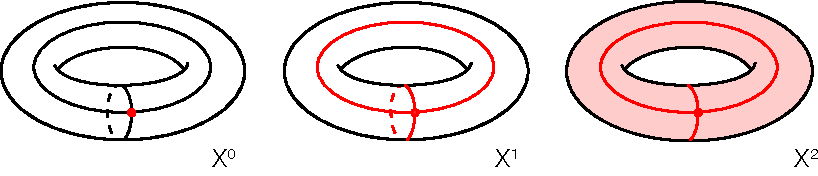
\includegraphics[width=0.8\textwidth ]{resources/chap_misc/torus_skeleton.pdf}  
	\caption{Skeletons of a torus.}
	\label{fig:torus_skeleton}
\end{figure}
\begin{figure}[htb!]
	\centering  
	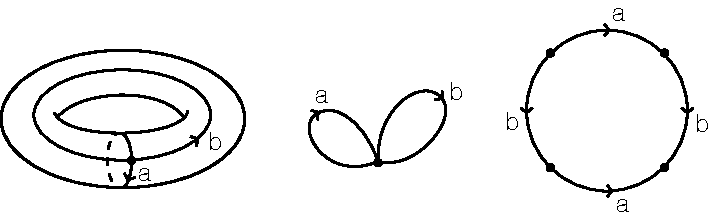
\includegraphics[width=0.7\textwidth ]{resources/chap_misc/torus_map.pdf}  
	\caption{Map from $S^2$ to $X^1$ of a torus.}
	\label{fig:torus_map}
\end{figure}

\begin{example}
	A orientable surface $M_g$ with genius $g$ is a surface with $g$ holes, as shown in Fig. \ref{fig:genus_g}.
\end{example}
\begin{figure}[htb!]
	\centering  
	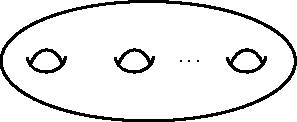
\includegraphics[width=0.4\textwidth ]{resources/chap_misc/genus_g.pdf}  
	\caption{A orientable surface $M_g$ with genius $g$.}
	\label{fig:genus_g}
\end{figure}

\begin{example}
	$M_g$ is a 2D CW complex. The way to attach 2-cell to $X^1$ is shown in \ref{fig:genus_g_map}.
\end{example}
\begin{figure}[htb!]
	\centering  
	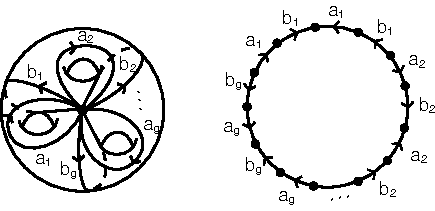
\includegraphics[width=0.6\textwidth ]{resources/chap_misc/genus_g_map.pdf}  
	\caption{Map from $S^2$ to $X^1$ of $M_g$. }
	\label{fig:genus_g_map}
\end{figure}

\part{Homotopy Group I}

\chapter{Basic Construction}

Note: all map in this part is assumed to be continuous.

\section{Homotopy and Homotopy type}

\begin{definition}
	A {\bf retraction} of a space $X$ onto a subspace $A\subseteq X$ is a surjective map $f:X\mapsto A$ such that $f|_A=1_A$.
\end{definition} 

\begin{definition}
	A {\bf homotopy} from $f_0:X\mapsto Y$ to $f_1:X\mapsto Y$ is a map $f:X\times I\mapsto Y$ such that $(\forall x\in X)(f(x,0)=f_0(x)\wedge f(x,1)=f_1(x))$, as shown in Fig. \ref{fig:homotopy}. Two maps $f_0$ and $f_1$ are {\bf homotopic} iff there exists a homotopy that connects them, written as $f_0\simeq f_1$.
\end{definition}

\begin{definition}
	Let $f:X\times I\mapsto Y$ be a homotopy. $f$ is a {\bf homotopy relative to} $A\subseteq X$ if $(\forall x\in A)f(x,t)$ is constant. If there exists a homotopy that connects $f_0$ and $f_1$ relative to $A$, we say $f_0\simeq f_1$ rel $A$.
\end{definition}

\begin{definition}
	Let $f:X\mapsto A$ be a retraction. A {\bf deformation retraction} of $X$ onto $A$ is a homotopy from $1_X$ to $f$ rel $A$.
\end{definition}

\begin{figure}[htb!]
	\centering  
	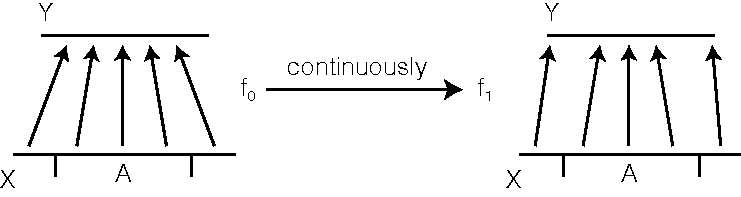
\includegraphics[width=0.7\textwidth ]{resources/chap_bas_cstr/homotopy.pdf}  
	\caption{A homotopy from $f_0$ to $f_1$ relative to $A$.}
	\label{fig:homotopy}
\end{figure}

\begin{definition}
	Space $X$ and $Y$ are said to be {\bf homotopy equivalent} or to have the same {\bf homotopy type}, written as $X\simeq Y$, if there's a map $f:X\mapsto Y$ and a map $g:Y\mapsto X$ such that $f\circ g\simeq 1_Y$ and $g\circ f\simeq 1_X$.
\end{definition}

\begin{definition}
	A space that has the homotopy type of a point is called {\bf contractible}.
\end{definition}

\section{Pointed Space}

\begin{definition}
	A {\bf pointed space} is a space with a distinguished point, the {\bf base point}. Space $X$ with based point $x_0$ is written as $(X,x_0)$, abbreviated by $X$. Continuous maps between pointed spaces that preserve the base points are called {\bf based maps}.
\end{definition}

\begin{definition}
	Let $\bar X=(X,x_0)$ and $\bar Y=(Y,y_0)$ be point spaces. We define there {\bf wedge sum} as $\bar X\vee \bar Y=(X\sqcup Y/(x_0\sim y_0),\overline{x_0})$
\end{definition}

\begin{definition}
	Let $(X,x_0)$ and $(Y,y_0)$ be point spaces, and $f_0:X\mapsto Y$ and $f_1:X\mapsto Y$ are based maps. A {\bf based point preserving homotopy} from $f_0$ to $f_1$ is a homotopy from $f_0$ to $f_1$ rel $x_0$.
\end{definition}

\begin{definition}
	Two point spaces $(X,x_0)$ and $(Y,y_0)$ are {\bf homotopic equivalent}, written as $(X,x_0)\simeq(Y,y_0)$, iff there's based maps $f:X\mapsto Y$ and $g:Y\mapsto X$ and based point preserving homotopies $f\circ g\simeq 1_Y$ and $g\circ f\simeq 1_X$.
\end{definition}

\begin{definition}
	Let $S^n=\{x\in\mathbb R^n|\sum_{i=0}^n x_i^2=1\}$ be a sphere.
	\begin{enumerate}
		\item The {\bf north hemisphere} of $S^n$ is $\{x\in S^n|x_0\geq0\}$.
		\item The {\bf south hemisphere} of $S^n$ is $\{x\in S^n|x_0\leq0\}$.
		\item The {\bf east hemisphere} of $S^n$ is $\{x\in S^n|x_1\geq0\}$.
		\item The {\bf west hemisphere} of $S^n$ is $\{x\in S^n|x_1\leq0\}$.
		\item The {\bf north pole} of $S^n$ is $(1,0,\cdots,0)$.
		\item The {\bf south pole} of $S^n$ is $(-1,0,\cdots,0)$.
		\item The {\bf equator} of $S^n$ is $\{x\in S^n|x_0=0\}$.
	\end{enumerate}
\end{definition}

\begin{lemma}
	Let $S^n$ be a $n$-sphere $(n\geq1)$ with south pole as its base point. The map $v=\iota\circ w:S^n\mapsto S^n\vee S^n$ is a based map, where $w:S^n\mapsto S^n\sqcup S^n$ defined by
	\begin{equation}
		w(x)=(2|x_1|-1,2\sqrt{\frac{|x_1|}{1+|x_1|}}x_0,2\sqrt{\frac{|x_1|}{1+|x_1|}}x_2,2\sqrt{\frac{|x_1|}{1+|x_1|}}x_3,\dots)
	\end{equation}
	maps the east hemisphere to the 1st sphere and the west hemisphere to the 2nd sphere, and $\iota$ is the quotient map $S^n\sqcup S^n\mapsto S^n\vee S^n$. The case $n=2$ is shown in Fig. \ref{fig:sphere}.
\end{lemma}

\begin{figure}[htb!]
	\centering  
	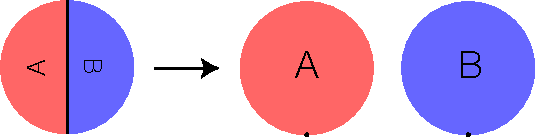
\includegraphics[width=0.5\textwidth ]{resources/chap_bas_cstr/sphere.pdf}  
	\caption{Based map from $S^2$ to $S^2\vee S^2$.}
	\label{fig:sphere}
\end{figure}

\begin{lemma}
	Let $S^n$ be a $n$-sphere $(n\geq1)$ with south pole as its base point. The following map $i:S^n\mapsto S^n$ is a based map.
	\begin{equation}
		i(x)=(x_0,-x_1,x_2,\dots)
	\end{equation}
\end{lemma}

\section{Homotopy Group}

\begin{definition}
	Let $X$ be a space. The {\bf $n$-loop} at $x_0\in X$ is a map $f:S^n\mapsto X$, that maps the south pole to $x_0$.
\end{definition}

\begin{definition}
	Let $f,g$ be two $n$-loops in $X$ at $x_0$, we define there wedge sum $f\vee g:S^n\bigvee S^n\mapsto X$ as
	\begin{equation}
		f\vee g(\bar x)=\left\{
		\begin{array}{cc}
			f(x)& x\in {\rm 1st\ } S^n\\
			g(x)& x\in {\rm 2nd\ } S^n
		\end{array}
		\right.
	\end{equation}
	where $f\vee g$ maps the base point of $S^n\bigvee S^n$ to $x_0$.
\end{definition}

\begin{definition}
	Let $f,g$ be two $n$-loops in $X$ at $x_0$. We define there composition loop $f\cdot g:S^n\mapsto X$ as
	\begin{equation}
		f\cdot g=(f\vee g)\circ v
	\end{equation}
\end{definition}

\begin{definition}
	Let $f$ be an $n$-loops in $X$ at $x_0$, we define its inverse loop $f^{-1}:S^n\mapsto X$ as
	\begin{equation}
		f^{-1}=f\circ i
	\end{equation}
\end{definition}

\begin{definition}
	Let $X$ be a space. We define the constant $n$-loop $e$ at $x_0$ to be the constant map from $S^n$ to $x_0$.
\end{definition}

\begin{lemma}
	Let $f$ be an $n$-loops in $X$ at $x_0$. Then $f\cdot f^{-1}\simeq e$ rel the south pole.  
\end{lemma}
\begin{proof}
	The homotopy map is 
	\begin{equation}
		F(x,t)=f\cdot f^{-1}(\cos(\theta(1-t)+\pi t),s_1\sin(\theta(1-t)+\pi t),s_2\sin(\theta(1-t)+\pi t),\cdots))
	\end{equation}
	where $x=(\cos\theta,s_1\sin\theta,s_2\sin\theta,\cdots)$ and $s_1^2+s_2^2+\cdots=1$. The process is shown in Fig. \ref{fig:homotopy_inverse}.
\end{proof}

\begin{figure}[htb!]
	\centering  
	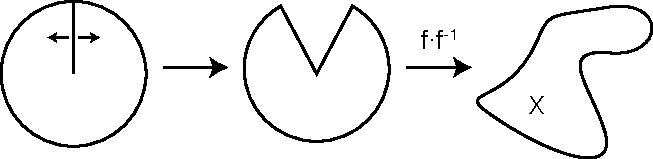
\includegraphics[width=0.6\textwidth ]{resources/chap_bas_cstr/invloop.pdf}  
	\caption{Homotopy when $0<t<1$.}
	\label{fig:homotopy_inverse}
\end{figure}

\begin{definition}
	Let $X$ be a space. The {\bf $n$-th homotopy group} (at $x_0$), written as $\pi_n(X,x_0)$, is the (base point preserving) homotopy types of all $n$-loops at $x_0$, with multiplication rule $[f]\cdot[g]=[f\cdot g]$, inverse $[f]^{-1}=[f^{-1}]$ and identity $[e]$. The 1st homotopy group is also called the {\bf fundamental group}.
\end{definition}

\begin{theorem}
	When $n\geq2$, the $n$-th homotopy group is abelian. So in this case we write $f\cdot g$ as $f+g$.
\end{theorem}

\begin{proof}
Let $f,g$ be two $n$-loops in $X$ at $x_0$. When $n\geq2$, we have a homotopy $f\cdot g\simeq g\cdot f$ rel the south pole:
	\begin{equation}
		F(x,t)=\left\{
		\begin{array}{cc}
			R_{12}(2\pi t)x&t\leq \frac 12\\
			R_{02}(\pi (2t-1))R_0(\pi)x&t>\frac 12
		\end{array}
		\right.
	\end{equation}
	where
	\begin{equation}
		R_{12}(\theta)(x_0,x_1,x_2,x_3,\cdots)=(x_0,x_1\cos\theta-x_2\sin\theta,x_2\cos\theta+x_1\sin\theta,x_3,\cdots)
	\end{equation}
	and
	\begin{equation}
		R_{02}(\theta)(x_0,x_1,x_2,x_3,\cdots)=(x_0\cos\theta-x_2\sin\theta,x_1,x_2\cos\theta+x_0\sin\theta,x_3,\cdots)
	\end{equation}
	
	The case $n=2$ is shown in Fig. \ref{fig:homotopy_abelian}.
\end{proof}

\begin{figure}[htb!]
	\centering  
	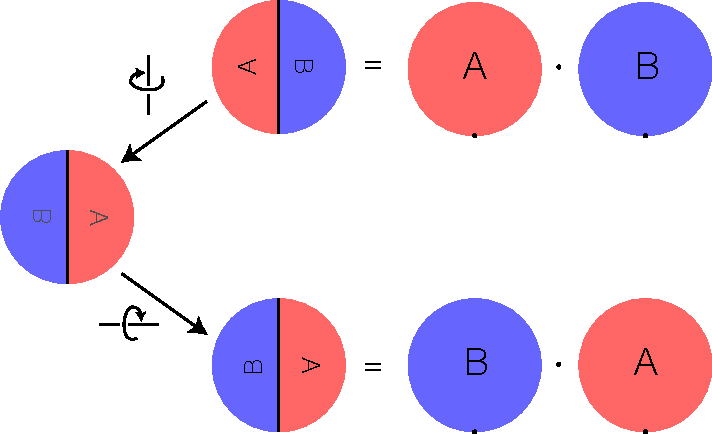
\includegraphics[width=0.7\textwidth ]{resources/chap_bas_cstr/homo_abelian.pdf}  
	\caption{Homotopy group is abelian.}
	\label{fig:homotopy_abelian}
\end{figure}

\begin{lemma}
	Let $X_\alpha$ be path-connected. Then $\pi_n(\prod_\alpha X_\alpha)\simeq \prod_\alpha\pi_n(X_\alpha)$.
\end{lemma}
\begin{proof}
	$[f]$ is mapped to $f'$ such that $f'_i=[f_i]$.
\end{proof}

\section{Change the Base Point}

\begin{definition}
	A {\bf path} in a space $X$ from $a$ to $b$ is a map $f:I\mapsto X$ such that $f(0)=a$ and $f(1)=b$. When we say a homotopy between paths, we always mean a homotopy relative to $\{0,1\}$. And for a path $f$ we use $[f]$ to denotes its homotopy type.
\end{definition}

\begin{definition}
	Let $f$ be a path in $X$. The {\bf inverse} of $f$ is the path $f^{-1}(t)=f(1-t)$.
\end{definition}

\begin{definition}
	Let $X$ be a path connected space. For each path $\gamma$ from $x_1$ to $x_0$ and each $[l]\in\pi_n(X,x_0)$, we define $\beta_{[\lambda]}:\pi_n(X,x_0)\mapsto\pi_n(X,x_1)$ by $\beta_{[\lambda]}([l])=[\bar \beta_\lambda(l)]$ where
	\begin{equation}
		\bar \beta_\lambda(l)(x)=\left\{
		\begin{array}{cc}
			l(2x_0-1,2\sqrt{\frac{x_0}{1+x_0}}x_1,2\sqrt{\frac{x_0}{1+x_0}}x_2,2\sqrt{\frac{x_0}{1+x_0}}x_3,\dots)&x_0>0\\
			\lambda(x_0+1)&x_0\leq0
		\end{array}
		\right.
	\end{equation}
	The case $n=2$ is shown in Fig. \ref{fig:change_base}.
\end{definition}

\begin{figure}[htb!]
	\centering  
	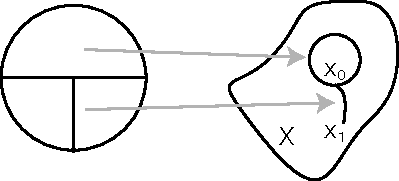
\includegraphics[width=0.4\textwidth ]{resources/chap_bas_cstr/change_base.pdf}  
	\caption{Change the base point from $x_0$ to $x_1$.}
	\label{fig:change_base}
\end{figure}

\begin{lemma}
	For each path $\lambda$ from $x_1$ to $x_0$, $\beta_{[\lambda]}$ is a group isomorphism from $\pi_n(X,x_0)$ to $\pi_n(X,x_1)$.
\end{lemma}
\begin{proof}
	Check $\beta_{[\lambda]}\beta_{[\lambda^{-1}]}=1$, $\beta_{[\lambda]}e=e$ and $\beta_{[\lambda]}(a+b)=\beta_{[\lambda]}a+\beta_{[\lambda]}b$.
\end{proof}

\begin{corollary}
	Let $X$ be a path connected space. Homotopy groups of $X$ at each point are isomorphic. So we may abbreviate $\pi_n(X,x_0)$ by $\pi_n(X)$.
\end{corollary}

\begin{corollary}
	For each $g\in \pi_1(X,x_0)$, $\beta_{g}$ is a group automorphism of $\pi_n(X,x_0)$.
\end{corollary}

\begin{definition}
	Let $\mathbb Z(\pi_1(X,x_0))$ be the group ring. We define the action of $\mathbb Z(\pi_1(X,x_0))$ on $\pi_n(X,x_0)$ $(n\geq2)$ as
	\begin{equation}
		(\sum_in_ig_i)f= \sum_in_i\beta_{g_i}f
	\end{equation}
	
	This makes $\pi_n(X,x_0)$ a $\mathbb Z(\pi_1(X,x_0))$ module.
\end{definition}

\section{Induced Homomorphisms}

\begin{definition}
	Let $(X,x_0)$ and $(Y,y_0)$ be point spaces, and $f:X\mapsto Y$ be a based map. Then $f$ induce a homomorphism $f_*:\pi_n(X,x_0)\mapsto\pi_n(Y,y_0)$ by $f_*([l])=[f\circ l]$.
\end{definition}

\begin{lemma}
	Let $\phi_t:X\mapsto Y$ be a base point preserving homotopy, then $\phi_{0*}=\phi_{1*}$.
\end{lemma}

\begin{lemma}
	Let $l$ be an $n$-loop at $x_0\in X$, and $f_t$ be a homotopy from $X$ to $Y$. Let $p=f_t(x_0)$ be a path from $f_0(x_0)$ to $f_1(x_0)$. Then $\bar \beta _{p^{-1}} (f_0\circ l)\simeq (f_1\circ l)$. The case $n=1$ is shown in Fig. \ref{fig:induce_hom}. Thus the following diagram commutes
	\[
	\begin{tikzcd}
		& \pi_n(Y,f_0(x_0))\arrow{d}{\beta_{[p^{-1}]}}
		\\
		\pi_n(X,x_0) \arrow{r}{f_{1*}} \arrow{ur}{f_{0*}}& \pi_1(Y,f_1(x_0))  
	\end{tikzcd}
	\]
\end{lemma}

\begin{corollary}
	Let $l$ be an $n$-loop at $x_0\in X$ and $f:X\mapsto X$ such that $f\simeq 1$ by $f_t$. Let $p=f_{t}(x_0)$ be a path from $f(x_0)$ to $x_0$. Then $f_*=\beta_{[p]}$.
\end{corollary}

\begin{figure}[htb!]
	\centering  
	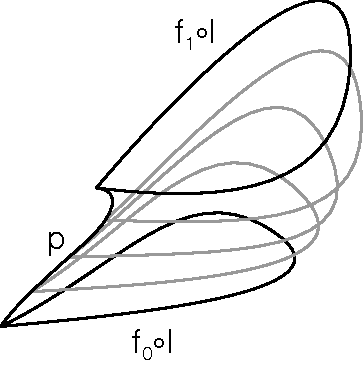
\includegraphics[width=0.3\textwidth ]{resources/chap_bas_cstr/induce_hom.pdf}  
	\caption{$\bar \beta _{p^{-1}} (f_0\circ l)\simeq (f_1\circ l)$.}
	\label{fig:induce_hom}
\end{figure}

\begin{lemma}
	Let $f:X\mapsto Y$ and $g:Y\mapsto X$. If $f\circ g\simeq 1$, then $f_*:\pi_n(X,x_0)\mapsto\pi_n(Y,f(x_0))$ is surjective for all $x_0\in X$. If $g\circ f\simeq 1$, then $f_*$ is injective.
\end{lemma}
\begin{proof}
	If $f\circ g\simeq 1$, $f_*g_*=\beta_h$ is bijective. So $f_*$ is surjective. If $g\circ f\simeq 1$, $g_*f_*=\beta_{h'}$ is bijective. So $f_*$ is injective.
\end{proof}

\begin{corollary}
	If a space $X$ retract onto a subspace $A$. Then $i_*:\pi_n(A,x_0)\mapsto\pi_n(X,x_0)$ induced by $i:A\hookrightarrow X$ is injective. If $A$ is a deformation retract of $X$, then $i_*$ is an isomorphism.
	
\end{corollary}

\chapter{Fundamental Group}
\section{Covering Spaces}

\begin{definition}
	Let $X$ be a path connected space. As illustrated in Fig. \ref{fig:cover_space}, $\tilde X$ is call a {\bf covering space} of $X$ if there's a map $p:\tilde X\mapsto X$ (called the {\bf covering map}) such that for each $x\in X$, there's an neighborhood $U$ of $x$ such that $p^{-1}(U)$ is a union of disjoint sets (named {\bf sheets}) in $\tilde X$, each of which is mapped homeomorphically onto $U$ by $p$. Such $U$ is called {\bf evenly covered}.
\end{definition}

\begin{figure}[htb!]
	\centering  
	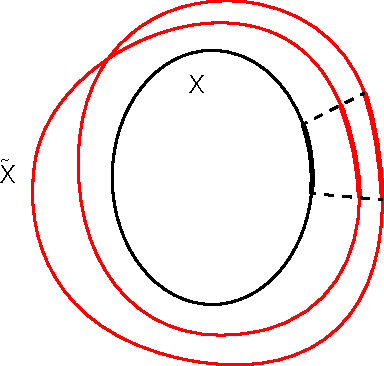
\includegraphics[width=0.3\textwidth]{resources/chap_fund_grp/cover_spc.pdf}  
	\caption{Illustration of covering space.}
	\label{fig:cover_space}
\end{figure}

\begin{definition}
	Let $p:\tilde X\mapsto X$ be a covering space. For each map $f:Y\mapsto X$, $\tilde f:Y\mapsto \tilde X$ {\bf lifts} $f$ iff $f=p \circ \tilde f$. That is, the following diagram commutes.
	
	\[
	\begin{tikzcd}
		& \tilde X\arrow{d}{p}
		\\
		Y \arrow{r}{f} \arrow{ur}{\tilde f}& X  
	\end{tikzcd}
	\]
\end{definition}

\begin{lemma}
	Let $p:\tilde X\mapsto X$ be a covering space. For each path $f$ which is lifted to $\tilde f_1,\tilde f_2$, $f_1=f_2$ if $\tilde f_1$ and $\tilde f_2$ agree on one point.
\end{lemma}

\begin{lemma}
	Let $p:\tilde X\mapsto X$ be a covering space. Given a homotopy $F:Y\times I\mapsto X$ and a map $\tilde F_0:Y\times\{0\}\mapsto \tilde X$ that lifts $F|_{Y\times\{0\}}$, then there's a homotopy $\tilde F:Y\times I\mapsto \tilde X$ lifting $F$ such that $\tilde F|_{Y\times\{0\}}=\tilde F_0$.
\end{lemma}
\begin{proof}
	For each $y\in Y$ and each $0\leq t\leq 1$, we have an evenly covered open basic neighborhood $N_i\times I_i \ni (y,t)$, where $I_i$ covers $I$. There's a finite subcover of $I_i$. Then we have $0=t_0<\cdots<t_n=1$ and open $N\ni y$, such that each $N\times [t_i,t_{i+1}]$ is in some evenly covered open set $U_{N,i}$. Then it's easy to construct a lift $F_N$ of $F$ on $N\times I$. From the last lemma we see that $F_N(y)$ is the same for each $N$ and is unique. Thus we can define a unique lift $\tilde F$ of $F$.
\end{proof}

\begin{corollary}
	Let $p:\tilde X\mapsto X$ be a covering space. For each path $f:I\mapsto X$ starting at $x_0$ and each $\tilde x_0\in p^{-1}(x_0)$, there's a unique lift $\tilde f$ of $f$ starting at $\tilde x_0$. 
\end{corollary}

\begin{corollary}
	Let $p:\tilde X\mapsto X$ be a covering space. For each homotopy of paths $f:I\times I\mapsto X$ starting at $x_0$ (which means that $\forall t(f(t,0)=x_0)$) and each $\tilde x_0\in p^{-1}(x_0)$, there's a unique lift $\tilde f$ of $f$ starting at $\tilde x_0$ which is a homotopy in $\tilde X$. 
\end{corollary}
\begin{proof}
	Since $f(t,1)$ is constant, $\tilde f(t,1)$ must be constant.
\end{proof}

We can study the lift of a more general map. 
\begin{lemma}
	Let $p:(\tilde X,\tilde x_0)\mapsto (X,x_0)$ be a covering space. Given a map $f:(Y,y_0)\mapsto (X,x_0)$ with $Y$ path-connected and locally path-connected. Then a lift $\tilde f:(Y,y_0)\mapsto (\tilde X,\tilde x_0)$ of $f$ exits iff $f_*(\pi_1(Y,y_0))\subseteq p_*(\pi_1(\tilde X,\tilde x_0))$.

\end{lemma}
\begin{proof}
	Assume $f_*(\pi_1(Y,y_0))\subseteq p_*(\pi_1(\tilde X,\tilde x_0))$. For each $y\in Y$, let $p$ be a path from $y_0$ to $y$. Let $q=f\circ p$ be a path in $X$ from $x_0$ to $f(y)$. Let $\tilde q$ be the lift of $q$ starting at $\tilde x_0$. We define $\tilde f(y)=\tilde q(1)$.
	
	We first prove that $\tilde f(y)$ is well-defined. Let $p$ and $p'$ be two paths $y_0$ to $y$, and $q=f\circ p$ and $q'=f\circ p'$. Let $l$ be the loop in $\tilde X$ such that $p_*([l])=[p\circ l]=[q\cdot q'^{-1}]\in f_*(\pi_1(Y,y_0))$. Let $\tilde q$ and $\tilde q'$ be the lifts of $q$ and $q'$. There's a homotopy in $X$ from $p\circ l$ to $q\cdot q'^{-1}$, which lifts a homotopy from $l$ to $t$. Then there's a homotopy in $X$ from $q$ to $q\cdot q'^{-1}\cdot q'$, which lifts to a homotopy from $\tilde q$ to $t\cdot \tilde q'$. Then clearly $\tilde q(1)=\tilde q'(1)$.
	
	To see that $\tilde f$ is continuous, let $U\subseteq X$ be an open neighborhood of $f(y)$ having a lift $\tilde U\subseteq \tilde X$ containing $\tilde f(y)$ such that $p: \tilde U\mapsto U$ is a homeomorphism. Choose a path-connected open neighborhood $V$ of $y$ with $f(V)\subseteq U$. It can be proved that $\tilde f(V)\subseteq \tilde U$.
\end{proof}

We can also prove that the lift is unique. 
\begin{lemma}
	Let $p:\tilde X\mapsto X$ be a covering space. Given a map $f:Y\mapsto X$ with $Y$ connected. Let $\tilde f_1$ and $\tilde f_2$ be two lifts of $f$. If $\tilde f_1$ and $\tilde f_2$ agree on one point of $Y$, they must agree on all of $Y$.
\end{lemma}
\begin{proof}
	For each $y\in Y$, let $U\ni f(y)$ be an evenly covered open set, covered by $\{\tilde U_\alpha\}$. Let $\tilde f_1(y)\in U_1$ and $\tilde f_2(y)\in U_2$. There exists a neighborhood $N$ of $y$ such that $\tilde f_1(N)\in U_1$ and $\tilde f_2(N)\in U_2$. If $\tilde f_1(y)=\tilde f_2(y)$, then $U_1=U_2$. It's easy to see that $(\forall y\in N)\tilde f_1(y)=\tilde f_2(y)$. If $\tilde f_1(y)\neq\tilde f_2(y)$, then $U_1\neq U_2$. It's easy to see that $(\forall y\in N)\tilde f_1(y)\neq\tilde f_2(y)$. So the set that $\tilde f_1$ and $\tilde f_2$ agree on is both open and closed.
\end{proof}

\begin{lemma}
	Let $p:\tilde X\mapsto X$ be a covering space. Let $a$ and $b$ be two loops at $x_0\in X$. Let $\tilde a$ and $\tilde b$ be lifts of $a$ and $b$ starting at $\tilde x_0\in p^{-1}(x_0)$. Then $[a]=[b]$ iff $\tilde a(1)=\tilde b(1)$ and $[\tilde a]=[\tilde b]$. 
\end{lemma}

\begin{corollary}
	A covering map $p:(\tilde X,\tilde x_0)\mapsto( X, x_0)$ induce an injective map $p_*:\pi_1(\tilde X,\tilde x_0)\mapsto\pi_1( X, x_0)$. And $\{\{[p\cdot q]|q $ is a path from $\tilde x_0$ to $a\}|a\in p^{-1}(x_0)\}$ are right cosets of $p_*(\pi_1(\tilde X,\tilde x_0))$ in $\pi_1( X, x_0)$.
\end{corollary}

\begin{corollary}
	Let $p:\tilde X\mapsto X$ be a covering space. For each $\tilde x\in \tilde X$, let $l_{\tilde x}$ be a path from $\tilde x_0\in p^{-1}(x_0)$ to $\tilde x$. Then $\pi_1( X, x_0)=\{[p\circ l_{\tilde x}]|\tilde x\in p^{-1}(x_0)\}$.
\end{corollary}

\section{Fundamental Group of the Circle}

\begin{lemma}
	$\pi_1(S^1)=\mathbb Z$
\end{lemma}
\begin{proof}
	$\mathbb R$ is a covering space of $X$ with covering map $p:\mathbb R\mapsto S^1$ defined by $p(\theta)=(\cos\theta,\sin\theta)$. Let $f_n:I\mapsto \mathbb R$ be $f_n(t)=(\cos(2\pi nt),\sin(2\pi nt))$. It's easy to see that $\pi_1(S^1,(1,0))=\{[p\circ f_n]\}$ and $[p\circ f_n]\cdot[p\circ f_m]=[p\circ f_{n+m}]$.
\end{proof}

\begin{theorem}
	Every non-constant polynomial with coefficients in $\mathbb C$ has a root in $\mathbb C$.
\end{theorem}
\begin{proof}
	Let the polynomial be $p(z)=z^n+a_1 z^{n-1}+\cdots a_n$. Define a map
	\begin{equation}
		f_{r,t}(s)=\frac{p_t(re^{2\pi is})/p_t(r)}{|p_t(re^{2\pi is})/p_t(r)|}
		\label{eqn:s1_fund}
	\end{equation}
	where $p_t(z)=z^n+t(a_1 z^{n-1}+\cdots a_n)$ and $r,t,s\in I$.
	
	Fixing $r,t$, $f$ is a loop in $S^1\in\mathbb C$ based at $1$. Supposing $p$ has no roots, the formula is well-defined at $t=1$. When $|z|$ is large enough, $|z^n|>|a_1 z^{n-1}+\cdots a_n|$. So $p_t(z)$ has no roots with large $|z|$, and Eqn. \ref{eqn:s1_fund} is also well-defined when $r$ is large enough.
	
	First we fix $t=1$ and let $r$ goes from $0$ to a very large $r_0$. Then we fix $r$ and let $t$ goes from 1 to 0. This process describe a homotopy between $f_{0,1}(s)=1$ to $f_{r_0,0}(s)=e^{2\pi nis}$. There's a contradiction since $n>0$.
\end{proof}

\begin{lemma}
	There's no retraction $D^2\mapsto S^1=\partial D^2$.
\end{lemma}
\begin{proof}
	Each loop in $D^2$ is homotopic to a constant loop.
\end{proof}

\begin{theorem}
	Every continuous map $h:D^2\mapsto D^2$ has a fixed point.
\end{theorem}
\begin{proof}
	Suppose that there's no fixed point. For each $x\in D^2$, let $r(x)$ be the ray starting at $h(x)$ and passing through $x$. Let $f(x)\in S^1$ be the point that $r(x)$ leaves $D^2$. $f$ is a retraction $D^2\mapsto S^1=\partial D^2$.
\end{proof}

\begin{lemma}
	Let $f$ be a loop in $S^1$ such that $f(x)=-f(x+1/2)$. Then $[f]\neq 0$.
\end{lemma}
\begin{proof}
	Let $S^1$ is covering by $\mathbb R$ with the standard covering map $p:\mathbb R\mapsto S^1$. Let $\tilde f$ lifts $f$. Then $\tilde f(x+1/2)=\tilde f(x)+q(x)/2$ where $q(x)$ is an odd integer. Since $q(x)$ is continuous, it must be constant. So $\tilde f(x+1/2)=\tilde f(x)+q/2$ and thus $\tilde f(1)=\tilde f(0)+q$. So $[f]=[q]\neq0"$.
\end{proof}

\begin{theorem}
	For every continuous map $f:S^2\mapsto \mathbb R^2$, there exists a pair of antipodal points $x$ and $-x$ is $S^2$ with $f(x)=f(-x)$.
\end{theorem}

\begin{proof}
	If the conclusion is false, let $g(x)=(f(x)-f(-x))/|f(x)-f(-x)|$. Then $g$ maps $S^2$ to $S^1$ and $g(x)=-g(-x)$. Let $l$ be the loop circling the equation of the $S^2$. Then $q=g\circ l$ is a loop that $q(x)=-q(x+1/2)$. Since $l$ is homotopic to a constant loop, $[q]=0$, a contradiction.
\end{proof}

\section{The van Kampen Theorem}

\begin{theorem}[Serfeit, van Kampen]
	Let $X$ be the union of path-connected open sets $A_\alpha$ each containing the base point $x_0$. Let each intersection $A_\alpha\cap A_\beta$ be path-connected. Then the homomorphism $\Psi:* _\alpha \pi_1(A_\alpha)\mapsto \pi_1(X)$ defined by $\Psi([l_1][l_2]\cdots)=[l_1\cdot l_2\cdots]$ is surjective. If in addition each intersection $A_\alpha\cap A_\beta\cap A_\gamma$ is path-connected, then the kernel of $\Psi$ is the normal subgroup $N$ generated by all elements of the form $i_{\alpha\beta*}(\omega)i_{\beta\alpha*}(\omega)^{-1}$ for $\omega\in \pi_1(A_\alpha\cap A_\beta)$, and $i_{\alpha\beta}:A_\alpha\cap A_\beta\hookrightarrow A_\alpha$.
\end{theorem}
\begin{proof}
	The first part is evident. Let $l:I\mapsto X$ be a loop, then $I$ can be covered by finite open intervals, the image of each by $l$ lies in some $A_\alpha$.
	
	The second part needs more work. Clearly $N\in\ker\Psi$. Let $L=[l_1][l_2]\cdots$ and $L'=[l'_1][l'_2]\cdots$ such that $\Psi(l)=\Psi(l')$. There's a homotopy $F:I\times I\mapsto X$ from $l=l_1\cdot l_2\cdots$ to $l'=l'_1\cdot l'_2\cdots$. Due to the compactness of $I\times I$, one can fine $0=s_0<s_1<\cdots<s_m=1$ and $0=t_0<t_1<\cdots<t_n=1$ such that each rectangle $R_{ij}=[s_i,s_{i+1}]\times[t_i,t_{i+1}]$ is mapped to some single $A_{ij}$ by $F$. We perturb the vertical edge of the rectangles slightly so that each point in $I\times I$ lies in at most three rectangles. We may assume $A_{ij}\neq A_{i,j+1}$. Otherwise we can combine multiple rectangles into one rectangle. We can also require that $F$ maps vertical edge of the rectangles to $x_0$.
	
	For each horizontal row of rectangles $I\times[t_i,t_{i+1}]$, we have $L_i=[l_{i,1}]\cdot[l_{i,2}]\cdots\in* _\alpha \pi_1(A_\alpha)$, such that $[l_{i,j}]\in \pi_1(A_{ij})$ and $l_{i,1}\cdot l_{i,2}\cdots$ is homotopic to $l$. We want to study the relation between $L_i$ and $L_{i+1}$. For this purpose, we study the horizontal line $t=t_{i+1}$. Along this line, we can construct a combination of loops $p_{i1}\cdot p_{i2}\cdots$ which each loop  $p_{ij}$ is in both $ A_{\alpha_{ij}}$, the rectangle bellow $p_{ij}$, and $A_{\beta_{ij}}$, the rectangle above $p_{ij}$. It's easy to see $L_i=\prod_ji_{\alpha_{ij}\beta_{ij}}(p_{ij})$ and $L_{i+1}=\prod_ji_{\beta_{ij}\alpha_{ij}}(p_{ij})$. Since $\prod_ji_{\alpha_{ij}\beta_{ij}}(p_{ij})=\prod_ji_{\alpha_{ij}\beta_{ij}}(p_{ij})i^{-1}_{\beta_{ij}\alpha_{ij}}(p_{ij})i_{\beta_{ij}\alpha_{ij}}(p_{ij})$, it's easy to see that $L_i=L_{i+1}\cdot n$ where $n\in N$. Repeating this process, we can conclude that $L=L'\cdot n$ where $n\in N$. So $N=\ker\Psi$.
	
	The homotopy rectangle is shown in Fig. \ref{fig:vankampen_thm}.
	
\end{proof}

\begin{figure}[htb!]
	\centering  
	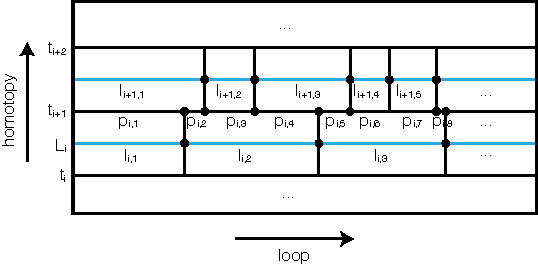
\includegraphics[width=0.9\textwidth ]{resources/chap_fund_grp/vankampen_thm.pdf}  
	\caption{The homotopy rectangle in proving the van Kampen theorem.}
	\label{fig:vankampen_thm}
\end{figure}


\begin{lemma}
	$\pi_1(\wedge_iX_i)=*_i\pi_1(X_i)$
\end{lemma}

\begin{lemma}
	$\pi_1(S^n)=0$ when $n\geq 2$.
\end{lemma}

\begin{example}
	In this example we calculate the fundamental group of a 2D CW complex.

	We attach a collection of 2-cells $e^2_\alpha$ to a path connected 1-skeleton $X^1$ via maps $\phi_\alpha:S^1\mapsto X_1$. Each $\phi_\alpha$ can be viewed as a loop in $X=X^2$. Let $\gamma_\alpha$ be a path from $x_0$ to $\phi_\alpha(0)$. Then $\eta_\alpha=\gamma_\alpha\phi_\alpha\gamma_\alpha^{-1}$ is a loop at $x_0$ in $X$.
	
	Let's expand $X$ to a slightly larger space $X'$ that deformation retracts onto $X$ by attaching rectangular strips $S_\alpha=I\times I$, with the lower edge attached to $\gamma_\alpha$, the right edge attached along an arc in $e_\alpha^2$, and all the left edges of the strips identified together, as shown in Fig. \ref{fig:cw_group}.
	
	 Let $C=\{c_\alpha\}$ be the set of centers of $e^2_\alpha$. Let $A=X'-C$ and $B=(X'-X)\cup \{x_0\}$. Then $A\cap B=(X'-X)\cup \{x_0\} -C$. It's easy to see that $B$ is contractable. So $\pi_1(X)\simeq\pi_1(X_1)/N$, where $N$ is the normal subgroup of $\pi_1(X)$ generated by $i(\omega)$ for $\omega\in\pi_1((X'-X)\cup \{x_0\} -C)$ and $i$ is the homomorphism induced by $A\cap B\hookrightarrow A$. It's easy to see that $\pi_1((X'-X)\cup \{x_0\} -C)$ is a free group generated by $[l_\alpha]$, where $l_\alpha$ deformation retracts onto a circle in $e^2_\alpha-\{c_\alpha\}$, as shown in Fig. \ref{fig:cw_group}. So $i([l_\alpha])=[\eta_\alpha]$. So $N$ is the normal subgroup generated by $[\eta_\alpha]$.
	 
	 \label{emp:cw_fund_grp}
\end{example}


\begin{figure}[htb!]
	\centering  
	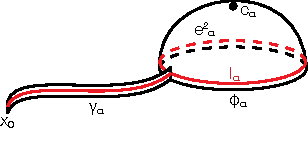
\includegraphics[width=0.5\textwidth ]{resources/chap_fund_grp/cw_group.pdf}  
	\caption{Strip attached to a CW complex.}
	\label{fig:cw_group}
\end{figure}

\begin{lemma}
	The fundamental group of $M_g$ is $\langle a_1,b_1,\cdots,a_g,b_g |[a_1,b_a]\cdots[a_g,b_g]\rangle$
\end{lemma}

\begin{lemma}
	For every group $G$ there is a 2D CW complex $X$ with $\pi_1(X)=G$. \label{lem:space_grp}
\end{lemma}
\begin{proof}
	Let $G=\langle g_\alpha|r_\beta\rangle$. We let $X_1$ be the wedge sum of circles representing $g_\alpha$s. For each $\beta$ we attach an $e_\beta^2$ to $X_1$ according to $r_\beta$
\end{proof}

\section{Classification of Covering Spaces}

\begin{definition}
	A path connected space $X$ is {\bf simply connected} iff $\pi_1(X)=0$.
\end{definition}

\begin{definition}
	A path connected space $X$ is {\bf locally simply connected} iff each point has a simply connected local neighborhood base.
\end{definition}

\begin{definition}
	A path connected space $X$ is {\bf semilocally simply connected} iff each point has a neighborhood $U$ such that every loop in $U$ is contractable in $X$.
\end{definition}

\begin{lemma}
	A path connected space $X$ is semilocally simply connected iff each point has a local neighborhood base containing sets in which every loop is contractable in $X$.
\end{lemma}

\begin{definition}
	A covering space is a {\bf universal cover} iff it's simply connected.
\end{definition}

\begin{lemma}
	A path-connected, locally path-connected, semilocally simply connected space $X$ has a universal cover.
\end{lemma}

\begin{proof}
	Let $x_0$ be a base point in $X$. Let $\tilde X$ be $\{[\eta]|\eta$ is a path in $X$ starting at $x_0 \}$. 
	
	We need to define a topology on $X$. For each $x\in X$, let $\mathcal U_x$ be a local neighborhood base at $x$, containing sets in which every loop is contractable in $X$. For each $[\eta]\in \tilde X$ and each $U_{\eta(1)}$ we define a set $N(U,[\eta])=\{[\eta\cdot\delta]|\delta$ is a path in $U$ starting at $\eta(1)\}$. Then we define a family $\mathcal U_{[\eta]}=\{N(U,[\eta])|U\in \mathcal U_{\eta(1)}\}$. It can be seen that $\mathcal U_{[\eta]}$ is a neighborhood base for a topology on $X$.
	
	Next we show the map $p:\tilde X\mapsto X$ defined by $p([\eta])=\eta(1)$ is a covering map. It's easy to see that $p$ is continuous. For each $x\in X$, choose an open $U_x\in\mathcal U_x$. It's easy to see that $\mathcal N_x=\{N(U_x,[\eta])|\eta$ is a path from $x_0$ to $x\}$ is a union of disjoint open sets and $\bigcup \mathcal N_x =p^{-1}(U_x)$.
	
	Finally we show that $\tilde X$ is simply connected. For this purpose, we study the lift of a path $\gamma$ starting at $x_0$ to a path $\tilde \gamma $ starting at $[x_0]$ (the homotopy type of a constant path). Let $\gamma_t$ be the path defined by 
	\begin{equation}
		\gamma_t(s)=\left\{\begin{array} {cc}
		\gamma(s)&s<t\\
		\gamma(t)&s\geq t
		\end{array} \right.
	\end{equation}
	We define $\tilde \gamma(t)=[\gamma_t]$. It's easy to see that $\tilde \gamma$ lifts $\gamma$, as shown in \ref{fig:lift_to_sp}. So $\tilde X$ is path-connected. $\tilde X$ is simply connected iff each loop $\xi$ in $\tilde X$, $p\circ\xi$ is contractable, which is clear since $\xi(1)=[p\circ\xi]=\xi(0)=[x_0]$.
\end{proof}

\begin{figure}[htb!]
	\centering  
	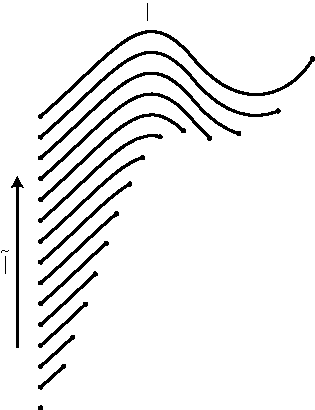
\includegraphics[width=0.3\textwidth ]{resources/chap_fund_grp/lift_to_sp.pdf}  
	\caption{Lift of a path to a universal cover.}
	\label{fig:lift_to_sp}
\end{figure}

\begin{lemma}
	Let $X$ be path-connected, locally path-connected and semilocally simply connected. Then for every subgroup $H\in \pi_1(X,x_0)$ there's a covering space $p_H:X_H\mapsto X$ such that ${\rm im}\ p_{H*}=H$.
\end{lemma}
\begin{proof}
	Let $p:\tilde X\mapsto X$ be the universal cover of $X$. Choose a $\tilde x_0\in p_H^{-1}(x_0)$. For each $\tilde x\in\tilde X$, we define $l_{\tilde x}$ to be a path from $\tilde x_0$ to $\tilde x$. We define a equivalence relation on $\tilde X$ by $\tilde x\sim \tilde y$ iff $p(\tilde x)=p(\tilde y)$ and $[(p\circ l_{\tilde x})\cdot (p\circ l_{\tilde y})^{-1}]\in H$. Especially $\tilde x\sim\tilde x_0$ iff $[(p\circ l_{\tilde x})]\in H$. We define $\tilde X_H=\tilde X/\sim$, and define $p_H:\tilde X_H\mapsto X$ by $p_H(\bar{\tilde x})=p(\tilde x)$. It's easy to see that $p_H$ is continuous. We define the natural map $q_H:\tilde X\mapsto\tilde X_H$. We have $p_H\circ q_H=1$.
	
	Next we prove that $p_H$ is a covering map. For each $x\in X$, let $U$ be an open set evenly covered by $\bigcup_\alpha U_\alpha$ in $\tilde X$. Let $p_\alpha:U_\alpha\mapsto U$ be the homomorphism. For each $\alpha\neq\beta$, if $(\exists u\in U)\overline{p_\alpha^{-1}(u)}=\overline{p_\beta^{-1}(u)}$, then $(\forall u\in U)\overline{p_\alpha^{-1}(u)}=\overline{p_\beta^{-1}(u)}$. Then it's easy to see that $p_H$ is a covering map.
	
	Finally we prove that ${\rm im}\ p_{H*}=H$. For each loop $l$ in $X$, let $\tilde l$ be the lift of $l$ in $\tilde X$. Then $l_H=q_H\circ \tilde l$ is the lift of $l$ in $X_H$. $[l]\in H$ iff  $\tilde l(1)\sim \tilde x_0$ iff $l_H$ is a loop in $X_H$ iff $[l]\in {\rm im}\ p_{H*}$.
\end{proof}

\begin{definition}
	Let $p_1:\tilde X_1\mapsto X$ and $p_2:\tilde X_2\mapsto X$ be two covering spaces. An {\bf isomorphism} from $\tilde X_1$ to $\tilde X_2$ is a homeomorphism $f:\tilde X_1\mapsto \tilde X_2$ such that $p_1=p_2\circ f$.
\end{definition}

\begin{lemma}
	Let $X$ be path-connected, locally path-connected and semilocally simply connected. Then two path-connected covering spaces $p_1:\tilde X_1\mapsto X$ and $p_2:\tilde X_2\mapsto X$ are isomorphic via $f:\tilde X_1\mapsto \tilde X_2$ taking a base point $\tilde x_1\in p^{-1}_1(x_0)$ to a base point $\tilde x_2\in p^{-1}_2(x_0)$ iff $p_{1*}(\pi_1(\tilde X_1,\tilde x_1))=p_{2*}(\pi_2(\tilde X_2,\tilde x_2))$.
\end{lemma}
\begin{proof}
	We may lift $p_1:\tilde X_1\mapsto X$ to $\tilde p_1:\tilde X_1\mapsto \tilde X_2$ and $p_2:\tilde X_2\mapsto X$ to $\tilde p_2:\tilde X_2\mapsto \tilde X_1$. By the unique lifting property, $\tilde p_1\circ \tilde p_2=1$ and $\tilde p_2\circ \tilde p_1=1$.
\end{proof}

\begin{corollary}
	Let $X$ be path-connected, locally path-connected and semilocally simply connected. Then two path-connected covering spaces $p_1:\tilde X_1\mapsto X$ and $p_2:\tilde X_2\mapsto X$ are isomorphic iff $p_{1*}(\pi_1(\tilde X_1))$ and $p_{2*}(\pi_2(\tilde X_2))$ are conjugate.
\end{corollary}

\section{Deck Transformations and Group Actions}

\begin{definition}
	For a covering space $p:\tilde X\mapsto X$ the isomorphisms $\tilde X\mapsto \tilde X$ are called {\bf deck transformations}. These form a a group $G(\tilde X)$ under composition.
\end{definition}

\begin{definition}
	A covering space $p:\tilde X\mapsto X$ is called {\bf normal} if for each $x\in X$ and each $\tilde x,\tilde x'\in p^{-1}(x)$ there's a deck transformation taking $\tilde x$ to $\tilde x'$.
\end{definition}

\begin{lemma}
	Let $p:(\tilde X,\tilde x_0)\mapsto(X,x_0)$ be a path-connected covering space of the path-connected, locally path-connected space $X$. This covering space space is normal iff $p_*(\pi_1(\tilde X,\tilde x_0))$ is a normal subgroup of $\pi_1(X,x_0)$
\end{lemma}

\begin{lemma}
	Let $p:(\tilde X,\tilde x_0)\mapsto(X,x_0)$ be a path-connected covering space of the path-connected, locally path-connected space $X$. $G(\tilde X)$ is isomorphic to $N(p_*(\pi_1(\tilde X,\tilde x_0)))/p_*(\pi_1(\tilde X,\tilde x_0))$.
\end{lemma}
\begin{proof}
	For each $[l]\in N(p_*(\pi_1(\tilde X,\tilde x_0)))$, let $\tilde l$ be the lift in $\tilde X$ from $\tilde x_0$ to $\tilde x_1$. Then $p_*(\pi_1(\tilde X,\tilde x_0))=p_*(\pi_1(\tilde X,\tilde x_1))$. Let $f([l])$ be the deck transformation mapping $\tilde x_0$ to $\tilde x_1$. $f$ is a homomorphism from $N(p_*(\pi_1(\tilde X,\tilde x_0)))$ to $G(\tilde X)$, with kernel $p_*(\pi_1(\tilde X,\tilde x_0))$.
\end{proof}

\begin{definition}
	Let $G$ be a group. The {\bf action} of $G$ on a topological space $X$ is a homomorphism from $G$ to the autohomeomorphism group of $X$. Let $X/G$ be the space of orbits with quotient topology. $X/G$ is called the {\bf orbit space}.
\end{definition}

\begin{lemma}
	Let $G$ be a group acting on $X$ that satisfies the condition:
	
	Each $x\in X$ has a neighborhood $U_x$ such that $(\forall g\neq h\in G)g(U_x)\cap h(U_x)=\emptyset$. 
	
	The quotient map $X\mapsto X/G$ is a normal covering space of $X/G$. If $X$ is path-connected, then $G$ is the deck transformation of this covering space. If $X$ is further locally path-connected, $\pi_1(X)=\pi_1(X/G)/G$.
\end{lemma}

\begin{definition}
	For each group $G=\langle g_\alpha|r_\beta\rangle$ we can define the {\bf Cayley graph} of $G$ as follows: The vertices are members of $G$. There's a directed edge joining $g$ and $h$ if there exists a generator $g_\alpha$ such that $gg_\alpha=h$.
\end{definition}

\begin{example}
	The Cayley graphs of $D_{12}=\langle a,b|a^{12}=1,b^2=1,abab=1\rangle$ and $\langle a,b\rangle$ are shown in Fig. \ref{fig:cayley_grp}.
\end{example}

\begin{figure}[htb!]
	\centering  
	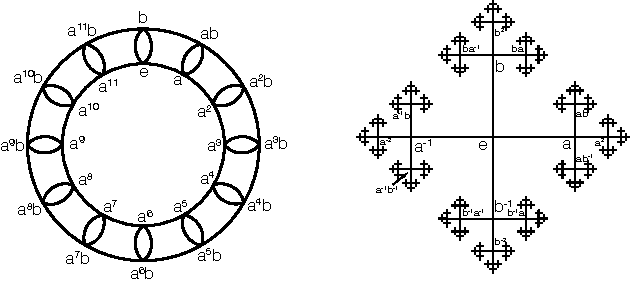
\includegraphics[width=0.8\textwidth ]{resources/chap_fund_grp/cayley_grph.pdf}  
	\caption{Left: Cayley graph of $D_{12}$. Right: Cayley graph of $\langle a,b\rangle$.}
	\label{fig:cayley_grp}
\end{figure}

\begin{definition}
	For each group $G=\langle g_\alpha|r_\beta\rangle$, let $C_G$ be the Cayley graph of $G$. For each $g\in G$ and each relation $r_\beta=e_1\cdots e_n$, $g\rightarrow ge_1\rightarrow\cdots\rightarrow(ge_1\cdots e_{n-1})\rightarrow g$ forms a loop, called $L(g,r_\beta)$. To each such loop we attach a $S^2$. The space we result in is called the {\bf Cayley complex} of $G$. 
\end{definition}

\begin{lemma}
	For each group $G=\langle g_\alpha|r_\beta\rangle$, let $\tilde X_G$ be the Cayley complex of $G$. $\tilde X_G$ is simply connected.
\end{lemma}
\begin{proof}
	Each loop in $C_G$ at $g$ can be decomposed by $P\rightarrow L(gh,r_1)\rightarrow\cdots\rightarrow L(gh,r_n)\rightarrow P^{-1}$, where $P$ is a path from $g$ to $gh$, since each $g_1\cdots g_m=1$ can be decomposed by $hr_1\cdots r_nh^{-1}$. Then use the Example \ref{emp:cw_fund_grp}.
\end{proof}

\begin{lemma}
	For each group $G=\langle g_\alpha|r_\beta\rangle$, let $C_G$ be the Cayley graph of $G$, and $\tilde X_G$ be the Cayley complex of $G$. We define the action of $G$ on vertices of $C_G$ by $g\cdot h=gh$. This action naturally extends to an action of $G$ on $\tilde X_G$. $X_G=\tilde X_G/G$ is just the space we define in Lem. \ref{lem:space_grp}.
\end{lemma}

\part{Homology and Cohomology}
\chapter{Simplicial Homology and Singular Homology}
\section{Simplicial Homology}

\begin{definition}
	An {\bf n-simplex} ($n>0$) denoted by and ordered n-tuple $[v_0,\dots,v_n]$ is the region $\{\sum_i\lambda_iv_i|\lambda_i>0,\sum_i\lambda_i=1\}$ in $\mathbb R^m$ ($m\geq n$), where $v_i$s are affine dependent vectors (not contained in any $n-1$ dimensional subspace) in $\mathbb R^m$. A $-1$-complex is defined as an empty set.
\end{definition}

\begin{definition}
	The {\bf faces} of a simplex $[v_0,\dots,v_n]$ are simplexes $[v'_0,\dots,v'_m]$ where $\{v'_0,\dots,v'_m\}\in\{v_0,\dots,v_n\}$.
\end{definition}

\begin{definition}
	An {\bf simplicial complex} $X$ is a set of simplexes with a map $f(\Delta,F)\mapsto\Delta'\in X$ for each $\Delta\in X$ and each face $F$ of $\Delta$, such that $F$ and $\Delta'$ are of the same dimension and that $F\neq F'\rightarrow f(\Delta,F)\neq f(\Delta,F')$
\end{definition}

In the following we will not distinguish between $F$ and $f(\Delta,F)$.

\begin{definition}
	Let $X$ be a simplicial complex. We define a {\bf simplicial n-chain} by
	\begin{equation}
		\cdots\overset{\partial_3}\longrightarrow C_2(X)\overset{\partial_2}\longrightarrow C_1(X)\overset{\partial_1}\longrightarrow C_0(X)\overset{\partial_0}\longrightarrow C_{-1}(X)=0
	\end{equation}
	, where $C_n(X)=\{$the free abelian group generated by all singular n-simplexes in $X\}$, and $\partial_n:C_n(X)\mapsto C_{n-1}(X)$ is a group homomorphism defined by
	\begin{equation}
		\partial_n [v_0,\dots,v_n]=\sum_i(-1)^i [v_0,\dots,\hat v_i,\dots,v_n]
	\end{equation}
	where $\hat v_i$ means that $v_i$ is omitted.
\end{definition}

\begin{theorem}
	$\partial_{n-1}\partial_n=0$
\end{theorem}

\begin{definition}
	Let $\cdots\rightarrow C_2(X)\rightarrow C_1(X)\rightarrow C_0(X)\rightarrow 0$ be a simplicial n-chain. We define {\bf simplicial n-cycles} as $Z_n(X)=\ker \partial_n$, and {\bf simplicial n-boundaries} as $B_n(X)={\rm im\ } \partial_{n+1}$. Clearly $B_n(X)\subseteq Z_n(X)$.
\end{definition}

\begin{definition}
	Let $\cdots\rightarrow C_2(X)\rightarrow C_1(X)\rightarrow C_0(X)\rightarrow 0$ be a simplicial n-chain. We define the nth {\bf simplicial homology group} of $X$ as $H_n(X)=Z_n(X)/B_n(X)$.
\end{definition}

\section{Singular Homology}
\begin{definition}
	Let $\Delta_n$ be an n-simplex for each $n\geq-1$. A {\bf singular n-simplex} in a topological space $X$ is a continuous map $\sigma:\Delta_n\mapsto X$. Especially $\Delta_{-1}$ is the empty map $\emptyset\mapsto X$.
\end{definition}

\begin{definition}
	Let $\Delta_n=[e_1,\dots,e_n]$ and $\Delta_{n-1}=[e'_1,\dots,e'_{n-1}]$. For each $i$ we define the ith {\bf face map} $\epsilon^n_i:\Delta_{n-1}\mapsto\Delta_n$ as $\epsilon^n_i(\sum_{j=0}^{n-1} t_j e'_j)=\sum_{j=0}^{i-1} t_j e_j+\sum_{j=i}^{n-1} t_j e_{j+1}$
\end{definition}

\begin{definition}
	Let $X$ be a topological space. We define a {\bf singular n-chain} by
	\begin{equation}
		\cdots\overset{\partial_3}\longrightarrow C_2(X)\overset{\partial_2}\longrightarrow C_1(X)\overset{\partial_1}\longrightarrow C_0(X)\overset{\partial_0}\longrightarrow C_{-1}(X)=0
	\end{equation}
	, where $C_n(X)=\{$the free abelian group generated by all singular n-simplexes in $X\}$, and $\partial_n:C_n(X)\mapsto C_{n-1}(X)$ is a group homomorphism defined by
	\begin{equation}
		\partial_n \sigma=\sum_i(-1)^i \sigma\circ \epsilon^n_i
	\end{equation}
\end{definition}

\begin{theorem}
	$\partial_{n-1}\partial_n=0$
\end{theorem}

\begin{definition}
	Let $\cdots\rightarrow C_2(X)\rightarrow C_1(X)\rightarrow C_0(X)\rightarrow 0$ be a singular n-chain. We define {\bf singular n-cycles} as $Z_n(X)=\ker \partial_n$, and {\bf singular n-boundaries} as $B_n(X)={\rm im\ } \partial_{n+1}$. Clearly $B_n(X)\subseteq Z_n(X)$.
\end{definition}

\begin{definition}
	Let $\cdots\rightarrow C_2(X)\rightarrow C_1(X)\rightarrow C_0(X)\rightarrow 0$ be a singular n-chain. We define the nth {\bf singular homology group} of $X$ as $H_n(X)=Z_n(X)/B_n(X)$.
\end{definition}

\part{Homotopy Group II}
%\appendix
% Here to insert appendix

%\printindex
%\bibliographystyle{unsrt}
%\bibliography{mybib}
\end{document}